
\documentclass[12pt,a4paper,oneside]{article}
\usepackage[margin=1.2in]{geometry}
\usepackage{appendix}
\usepackage[dvips]{graphicx}
\usepackage{epsfig}
\usepackage{amsmath}
\usepackage{amssymb}
\usepackage{psfrag}
\usepackage[square, comma,sort,numbers]{natbib}
\usepackage{fancyhdr}
\usepackage[nottoc]{tocbibind}
\usepackage{color}
\usepackage{fixltx2e}
\usepackage{pdfpages}
\usepackage{pdflscape}
\usepackage{booktabs}
\usepackage{graphicx}
\usepackage{float}
\usepackage{afterpage}
\usepackage{subcaption}
\usepackage{lscape}
\usepackage{rotating}
\usepackage{enumitem}
\usepackage{array,tabularx}
\usepackage{fancyref}
\usepackage{gensymb}
\usepackage[dvipsnames]{xcolor}
\usepackage[colorlinks=true,allcolors=blue]{hyperref}%



\newcommand{\quotes}[1]{``#1''}

\newenvironment{conditions*}
  {\par\vspace{\abovedisplayskip}\noindent
   \tabularx{\columnwidth}{>{$}l<{$} @{\ : } >{\raggedright\arraybackslash}X}}
  {\endtabularx\par\vspace{\belowdisplayskip}}



\pagestyle{fancy}
\title{\Huge The Hat Creek Radio Observatory\\
\vspace{0.5cm}
The RFSoC Digitizer Module\\
\vspace{0.5cm}
\normalsize \emph{}
\vspace{3.5cm}
\begin{center}

\includegraphics[height=4cm]{titlepage/SETI_institute_logo.jpg}
\end{center}
}
\author{ 
\vspace{1cm}
\Large
\textbf{ Alexander Pollak \& Sarah Schoultz} \\
SETI Institute \\ 
339 Bernardo Ave, Suite 200 \\
Mountain View, CA 94043 \\ 
Alexander.Pollak.87@gmail.com\\
}
\date{\today}



\begin{document}
\clearpage\maketitle
\thispagestyle{empty}

%\newpage
%\thispagestyle{empty}
%\section*{Abstract}
%\noindent 
%



%
%\vspace{3cm}
%\begin{flushright}
%Alexander Pollak \\ \emph{September, 2015}
%\end{flushright}

%\newpage
%\thispagestyle{empty}
%\tableofcontents
\newpage

%----------------------------------------------------------------------------------------
%	General
%----------------------------------------------------------------------------------------
%\pagestyle{plain}
\section{General}
\label{sec:1}
% ----------------------------------------------------------------
This document outlines general information regarding the RFSoC Digitizer Module such as the design, parts, wiring, and cabling. This information is aimed at detailing the entire process of creating an RFSoC Digitizer Module.

The purpose of an RFsoC Digitizer Module is to digitize the analog signals detected by the ATA's antennas. Once digitized, the signals can be saved and analyzed. This digitizer is a replacement for the ATA's previous digitizers called SNAPs and IBOBs. With sixteen 14-bit ADCs, two 100 G outputs, a larger FPGA, and more up to date technology, the RFSoC Digitizer Module is vast improvement upon the previous hardware. 


%----------------------------------------------------------------------------------------
%	CAD Design and Drawings
%--------------------------------------------------------------------------------------

\section{CAD Design and Drawings}
\label{sec:2}
% ----------------------------------------------------------------
This section includes a description of the RFSoC Digitizer Module's CAD design. An image of the CAD model is shown in Figure \ref{fig:CAD-Iso} and \ref{fig:CAD-top}. One can see the internal arrangement of the HTG-ZRF16 board (middle rear), power supply (front right), and directional fans (left rear and front right). The lid of the enclosure, not shown in this Figure, is perforated to further increase cooling. The panel facing the viewer in Figure \ref{fig:CAD-Iso} is considered the front panel. This is important to note for future sections. The majority of the RFSoC Digitizer Module's enclosure is off the shelf (PN: 24563-174) except for a few parts: the front panel, the back panel, the base plate, and the cable clamp. These custom parts were made by Front Panel Express, and the drawings can be found in Appendix A. 


%
\begin{figure}[H]
\centering
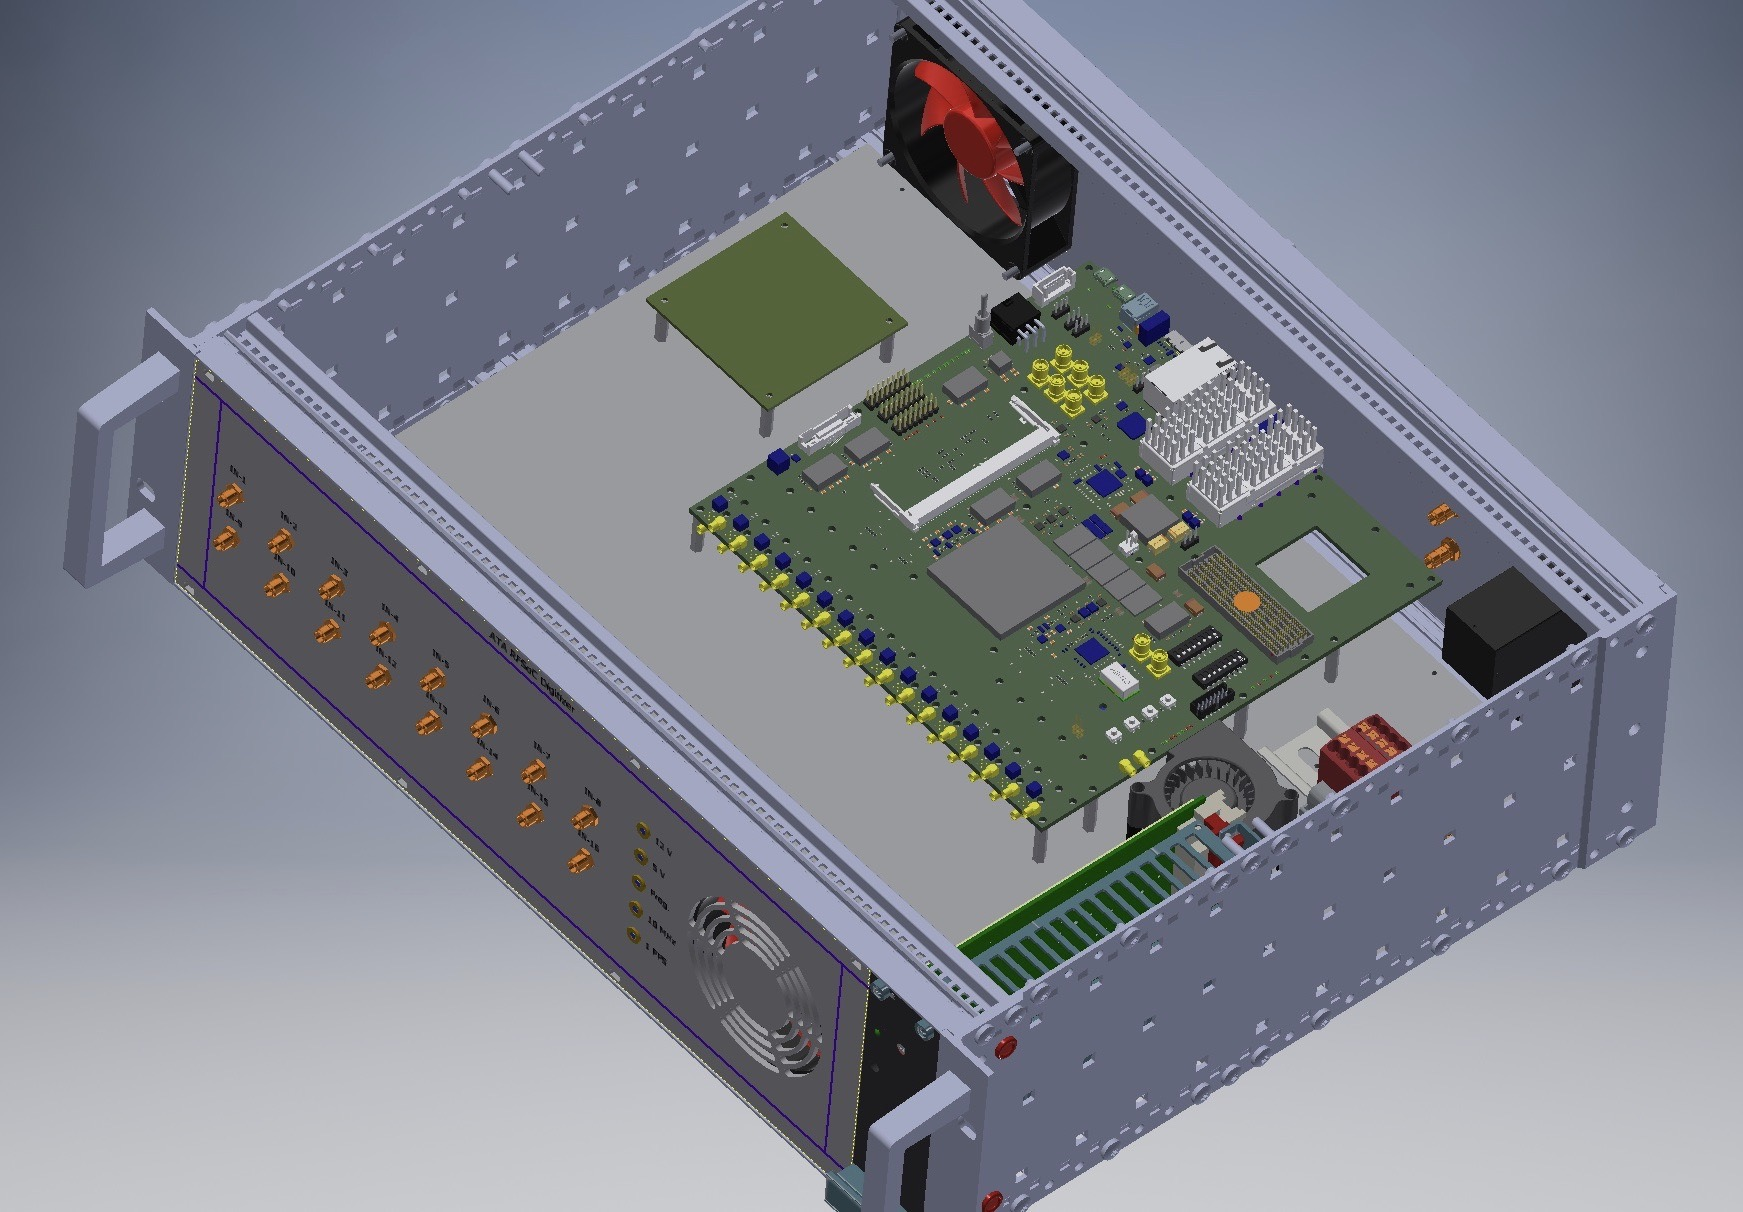
\includegraphics[width=.9\linewidth]{figures/CAD_iso.jpeg}
\caption{ISO view of the RFSoC CAD}
\label{fig:CAD-Iso}
\end{figure}
%

%
\begin{figure}[H]
\centering
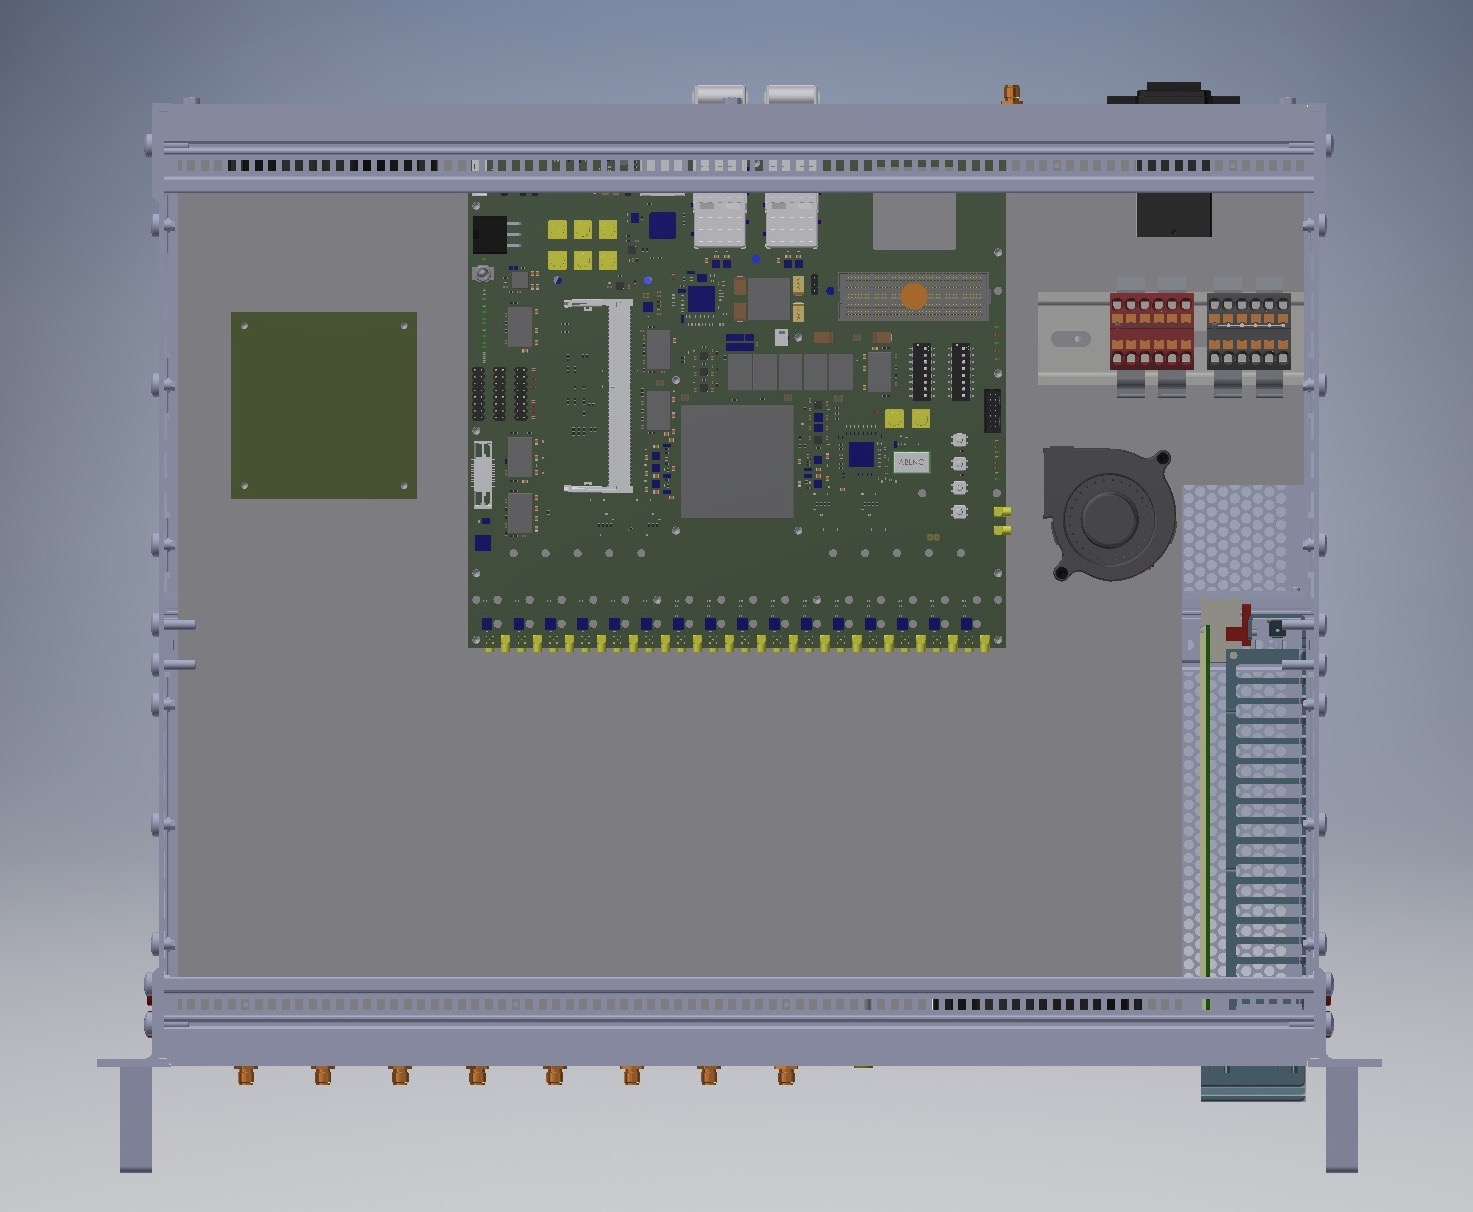
\includegraphics[width=.9\linewidth]{figures/CAD_top.jpeg}
\caption{Top View of the RFSoC CAD}
\label{fig:CAD-top}
\end{figure}
%

For a part list of the RFSoC Digitizer Module, except for the HTG-ZRF16 board and the  Interface Board,  see Appendix B. 

%----------------------------------------------------------------------------------------
%	HTG-ZRF16 Board
%---------------------------------------------------------------------------------------

\section{HTG-ZRF16 Board}
\label{sec:3}
% ----------------------------------------------------------------

The HTG-ZRF16 board, seen in Figure \ref{fig:HTG-ZRF16_Board}, is a product of HiTech Global. It is populated with a Xilinx ZYNQ UltraScale+ RFSoC ZU49DR FPGA. There are two on-board 100Gbps QSFP28 connectors allowing high-speed data processing via an optical interface. The board also has sixteen 14-bit ADCs with a sampling rate of 2.5 GSPS. 

%
\begin{figure}[H]
\centering
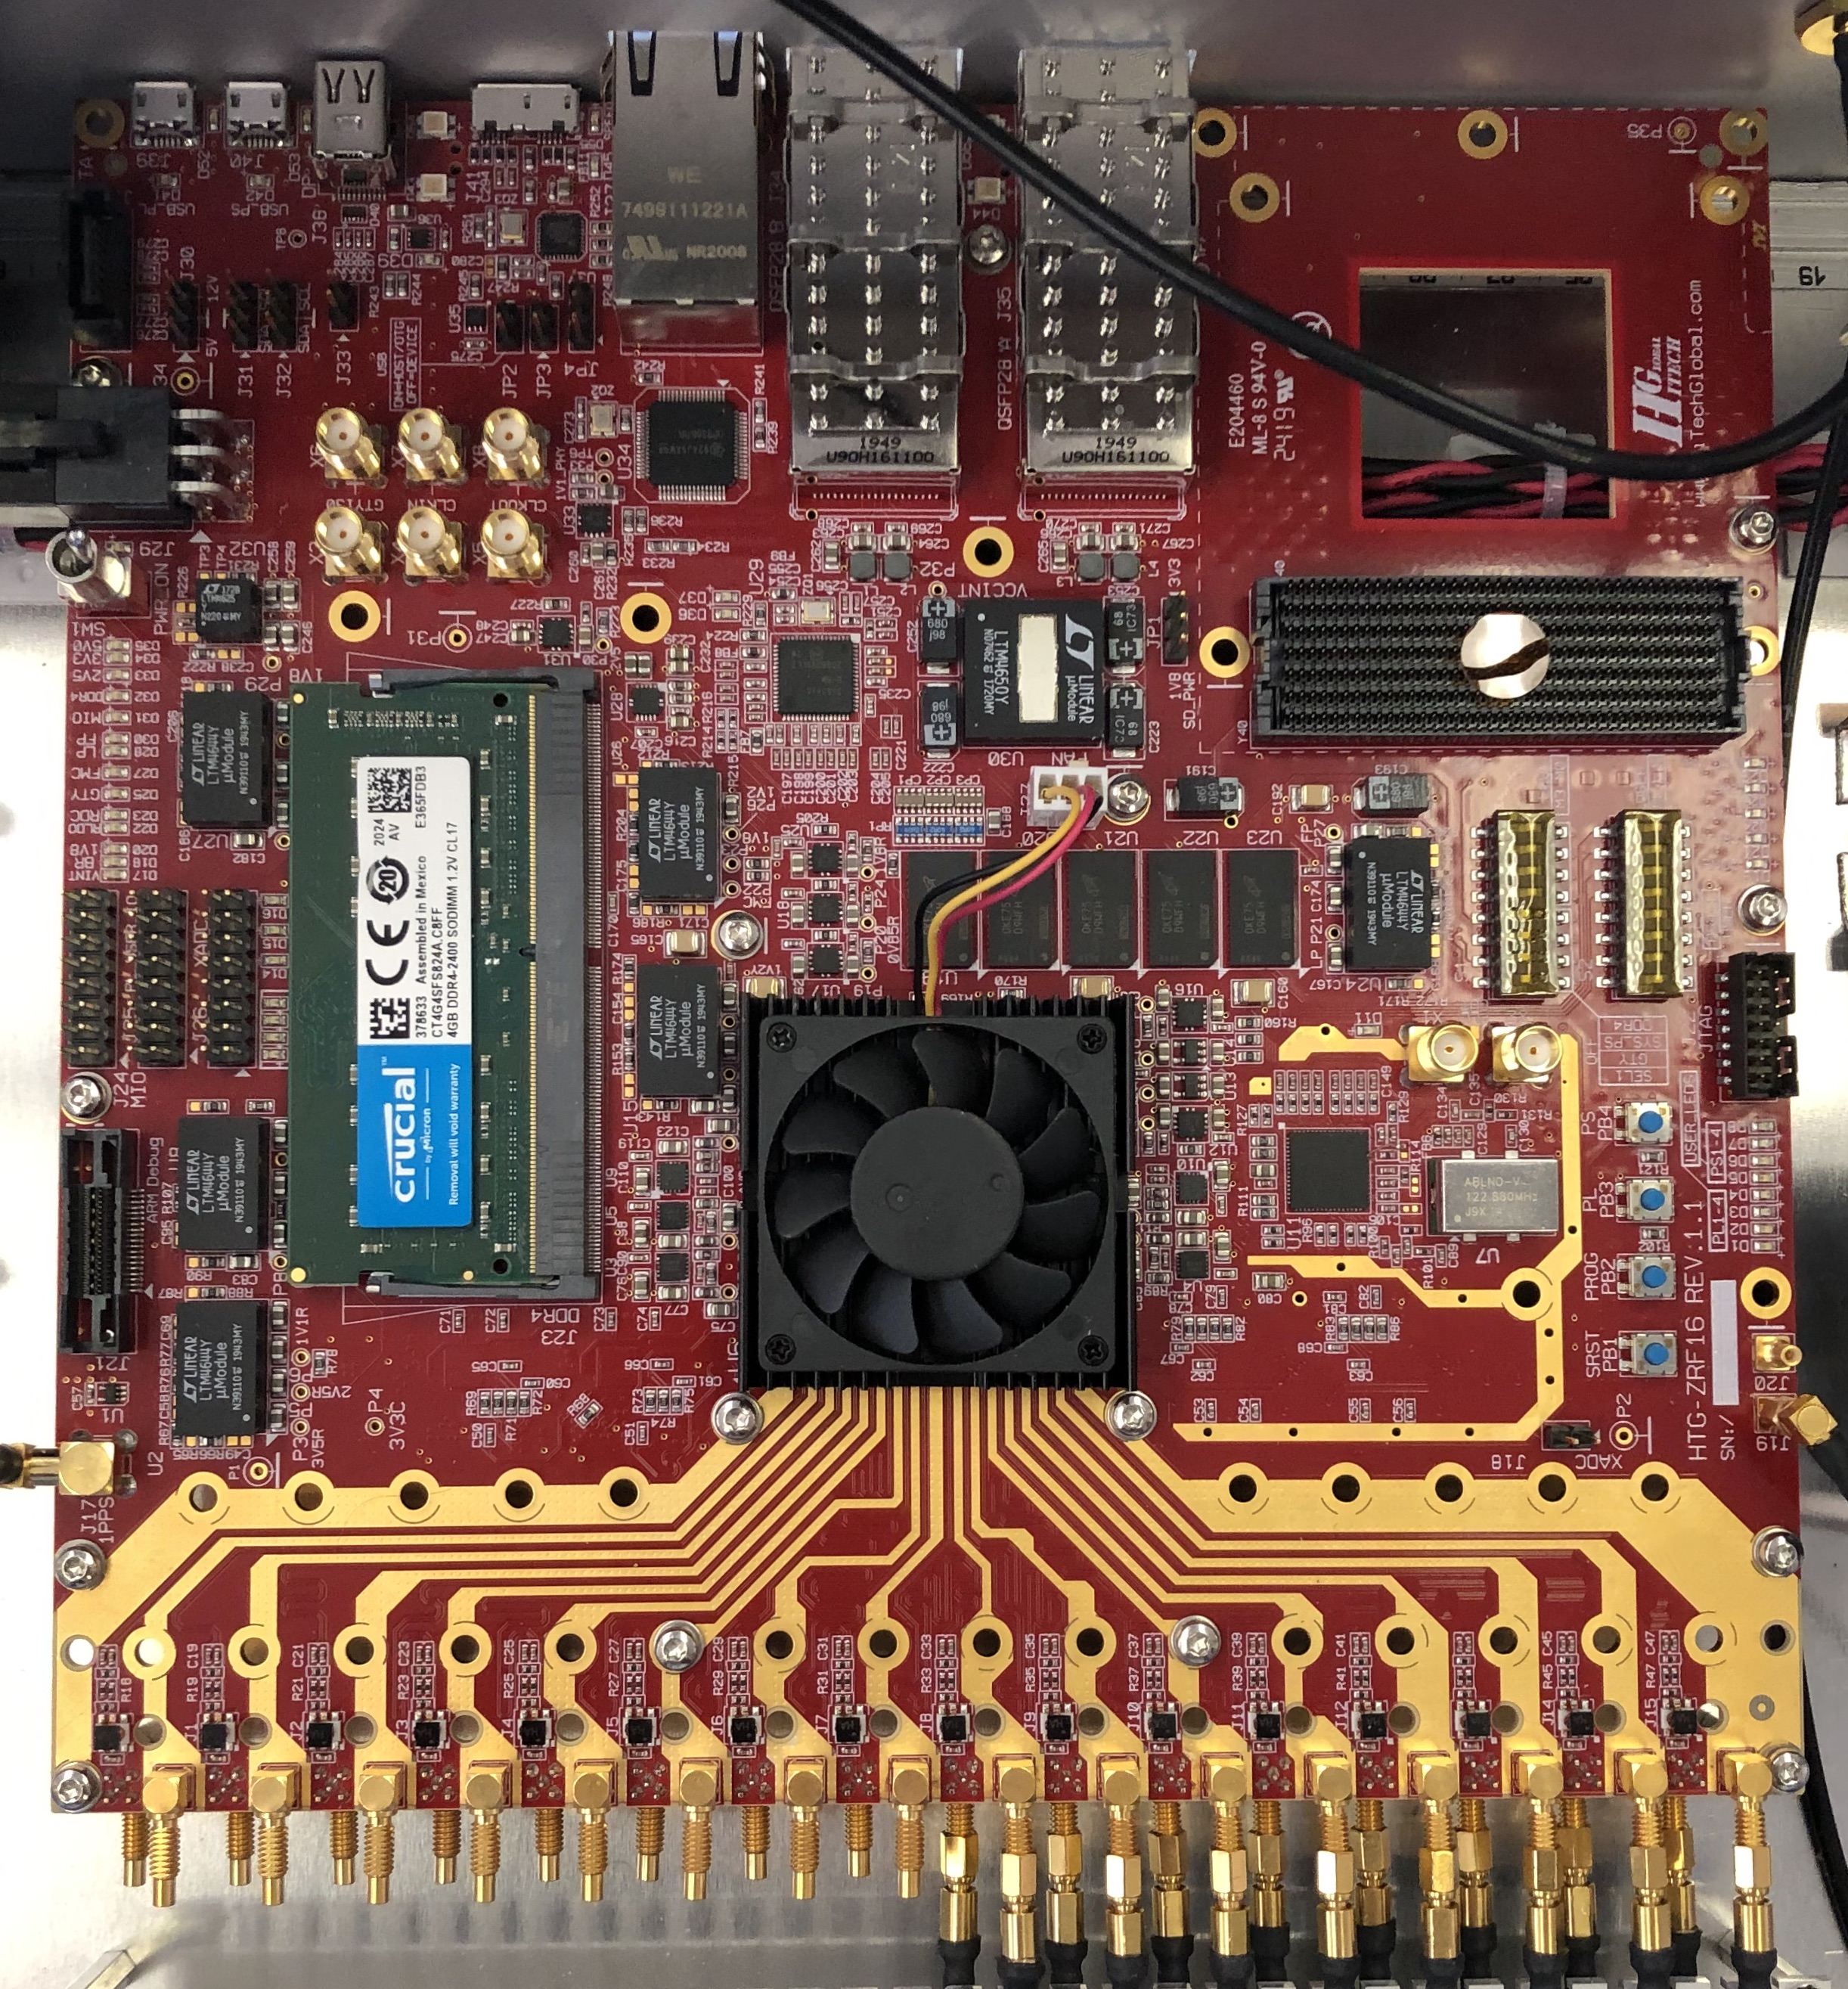
\includegraphics[width=1\linewidth]{figures/HiTech_Global_board.jpeg}
\caption{The HTG-ZRF16 Board Produced by HiTech Global}
\label{fig:HTG-ZRF16_Board}
\end{figure}
%

At the ATA, the RFSoC Digitizer Modules are operated at a sample rate of 2.048 GSPS. This is because the IF bandwidth is 700 MHz and centered at 512 MHz thus giving the system a 162 MHz leeway to prevent aliasing. Note that due to a known flaw, the HTG-ZRF16 boards purchased for the ATA were retrofitted by HiTech Global (Figure \ref{fig:Digitizer_retrofit}). Specifically, pin 44 (OSCin) of the LMK PLL chip was \emph{not} AC-coupled to ground as it should have been and was instead connected directly to ground. Hence, HiTech Global installed a capacitor in between pin 44 of the LMK PLL chip and ground as a retrofit for this issue. 

%
\begin{figure}[H]
\centering
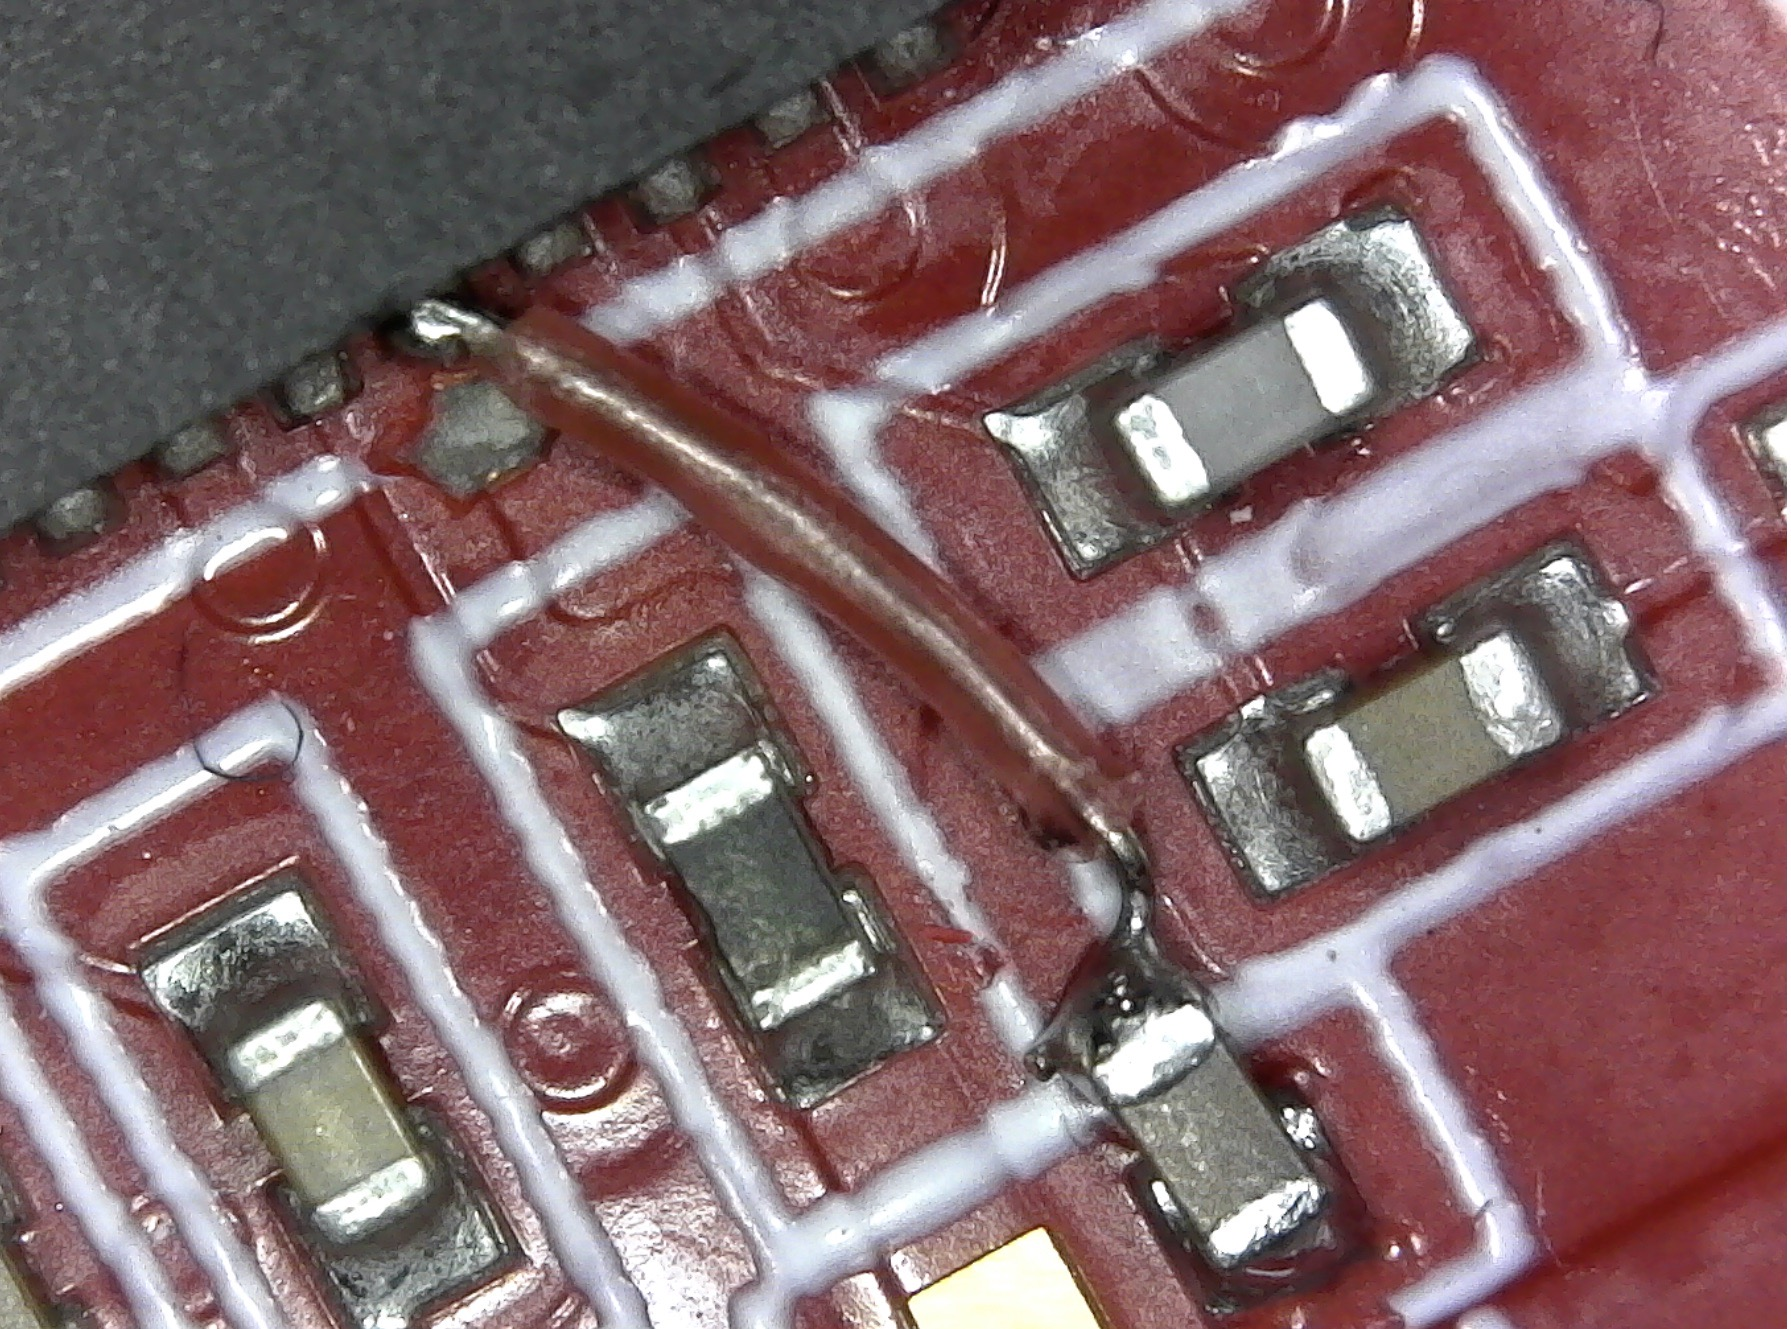
\includegraphics[width=1\linewidth]{figures/Digitizer_retrofit.jpeg}
\caption{The HTG-ZRF16 Board with Capacitor Retrofit on Pin 44 of the of the LMK PLL Chip}
\label{fig:Digitizer_retrofit}
\end{figure}
%

\subsection{Heat Sink Fan}
\label{sec:3.1}

While in use, the FPGA can reach high temperatures. Hence, the HTG-ZRF16 board comes with a heat sink fan mounted onto the FPGA (Figure \ref{fig:Old_heatsink_fan}). However, during initial use of the first RFSoC Digitizer Module, the temperature of the FPGA reached $90-95\degree C$ which is uncomfortably close to the FPGA's maximum temperature of $100\degree C$. It was, therefore, determined that the original heat sink fan was insufficient at keeping  the FPGA's temperature within acceptable levels and so was removed (Figure \ref{fig:FPGA}).

%
\begin{figure}[H]
\centering
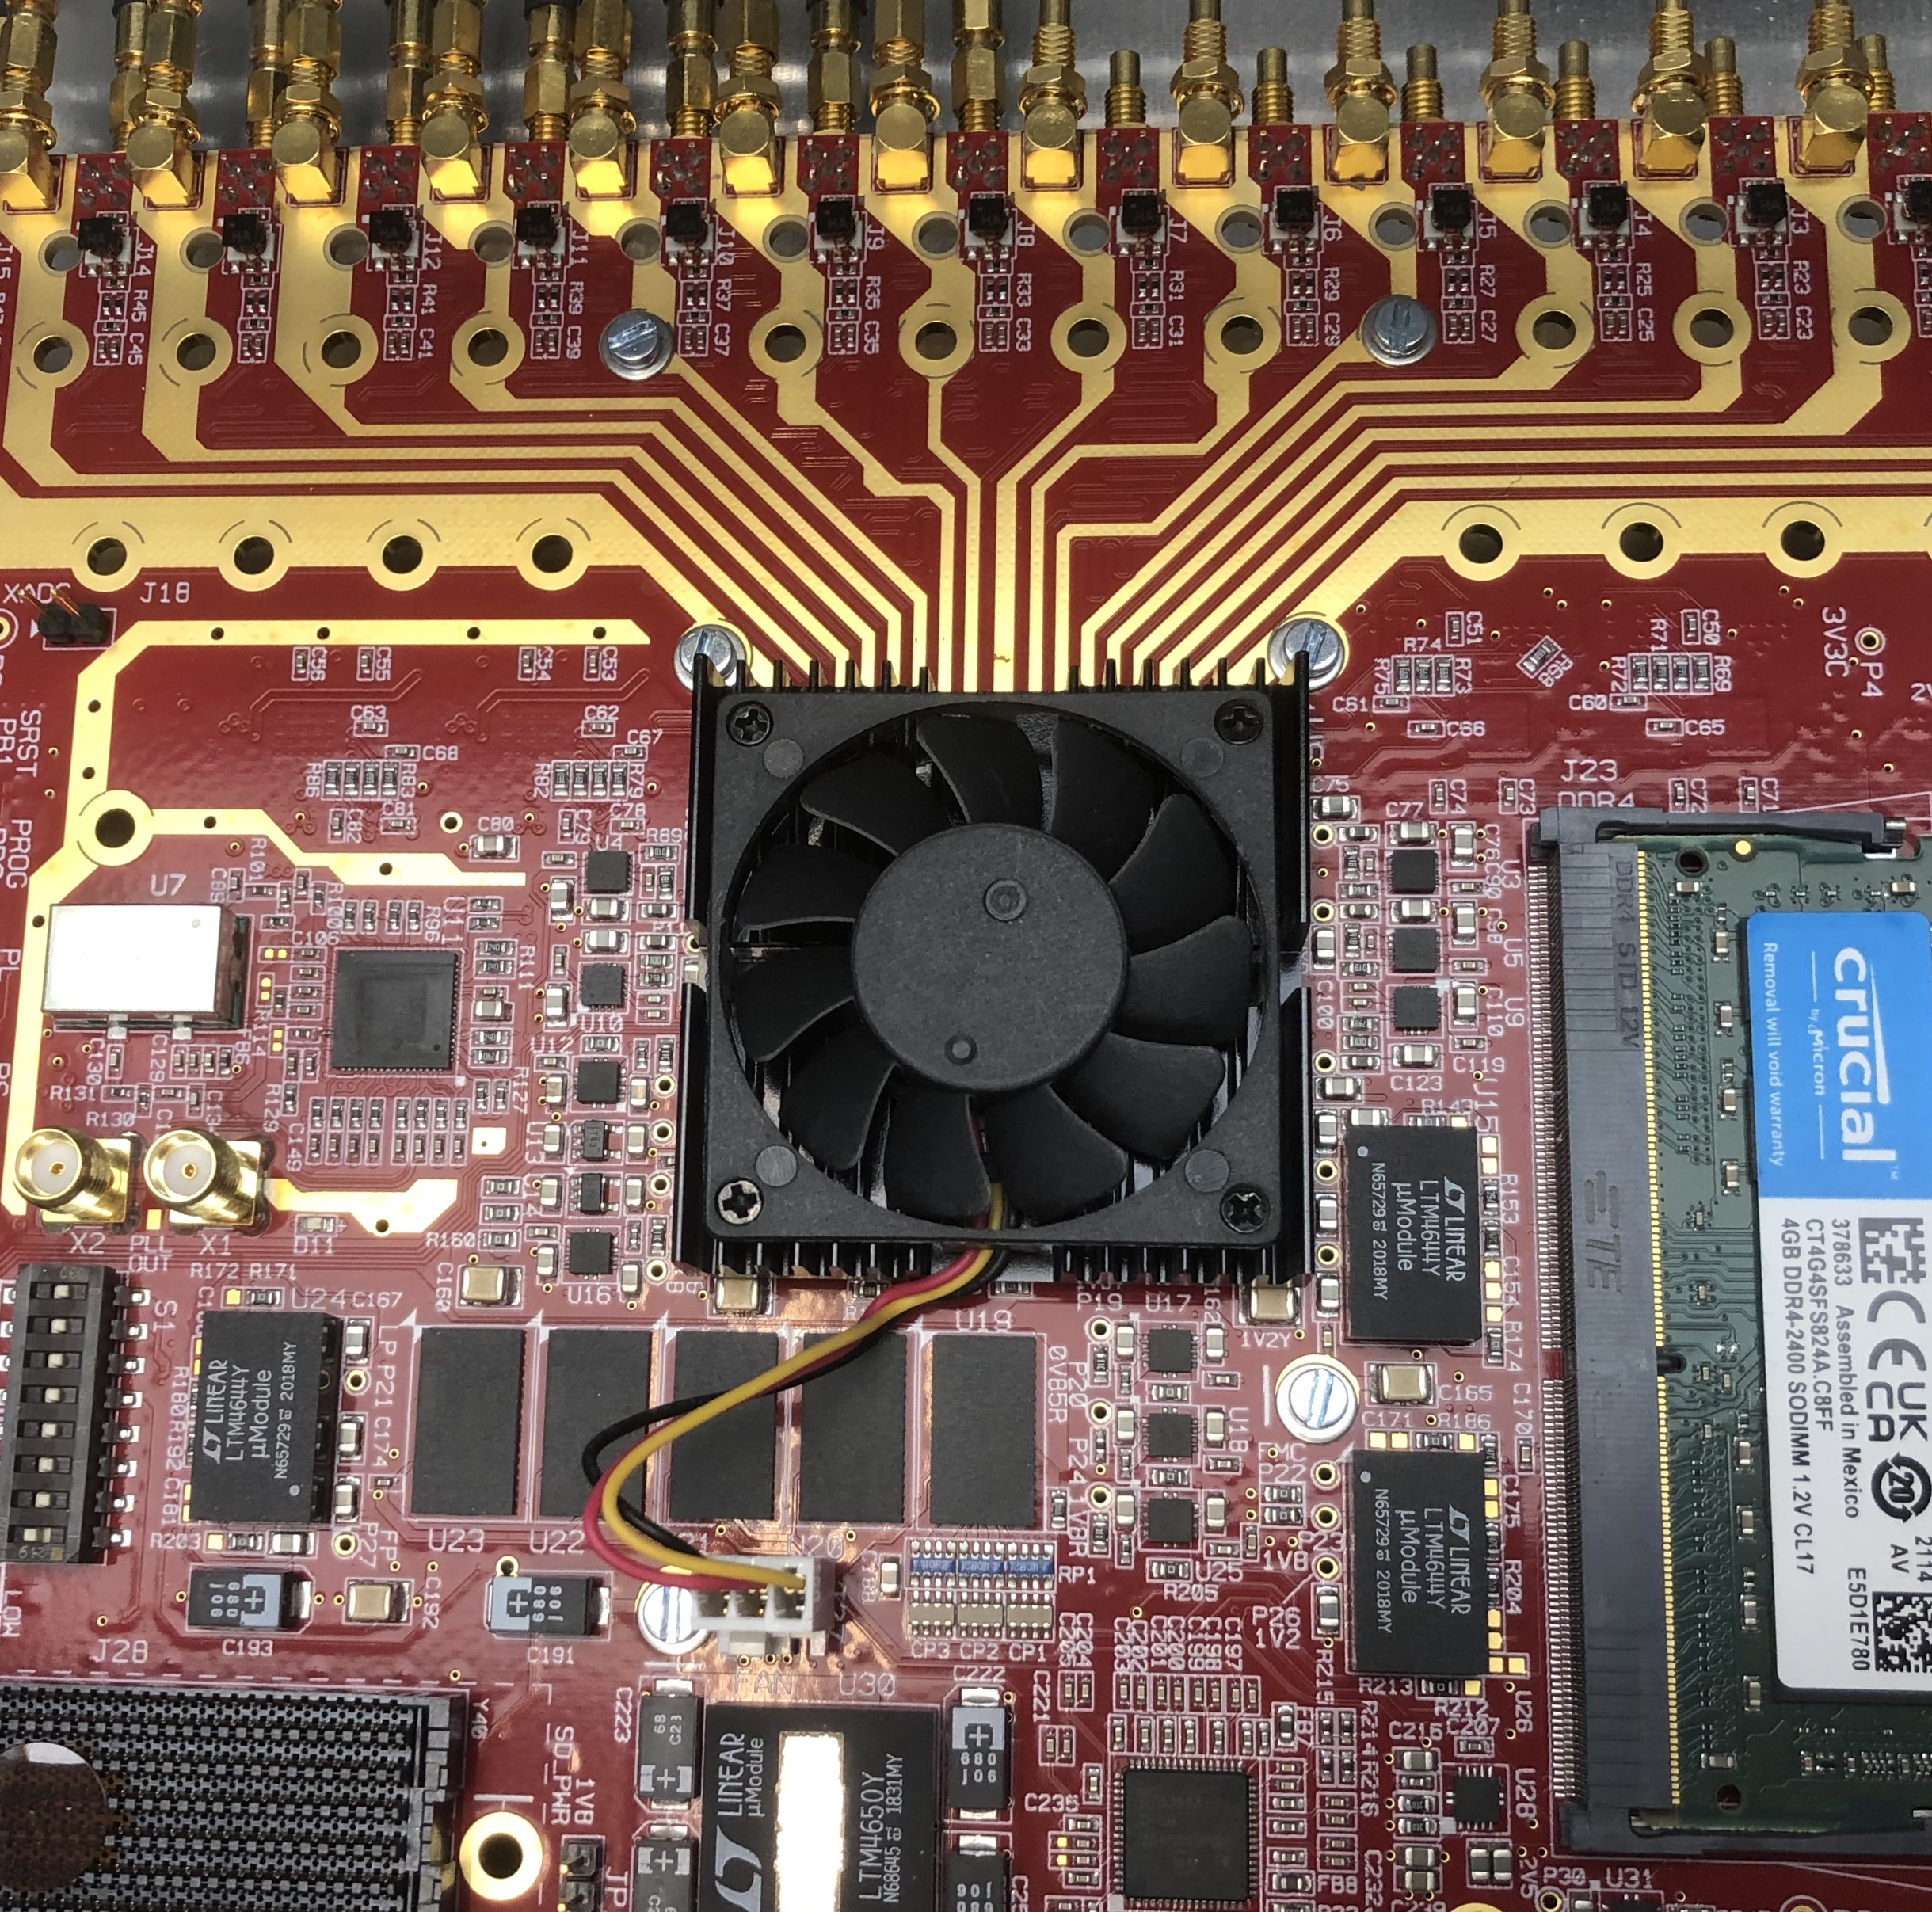
\includegraphics[width=.67\linewidth]{figures/Old_heatsink_fan.jpeg}
\caption{HTG-ZRF16 Board with the HiTech Global Heat Sink Fan}
\label{fig:Old_heatsink_fan}
\end{figure}
%

%
\begin{figure}[H]
\centering
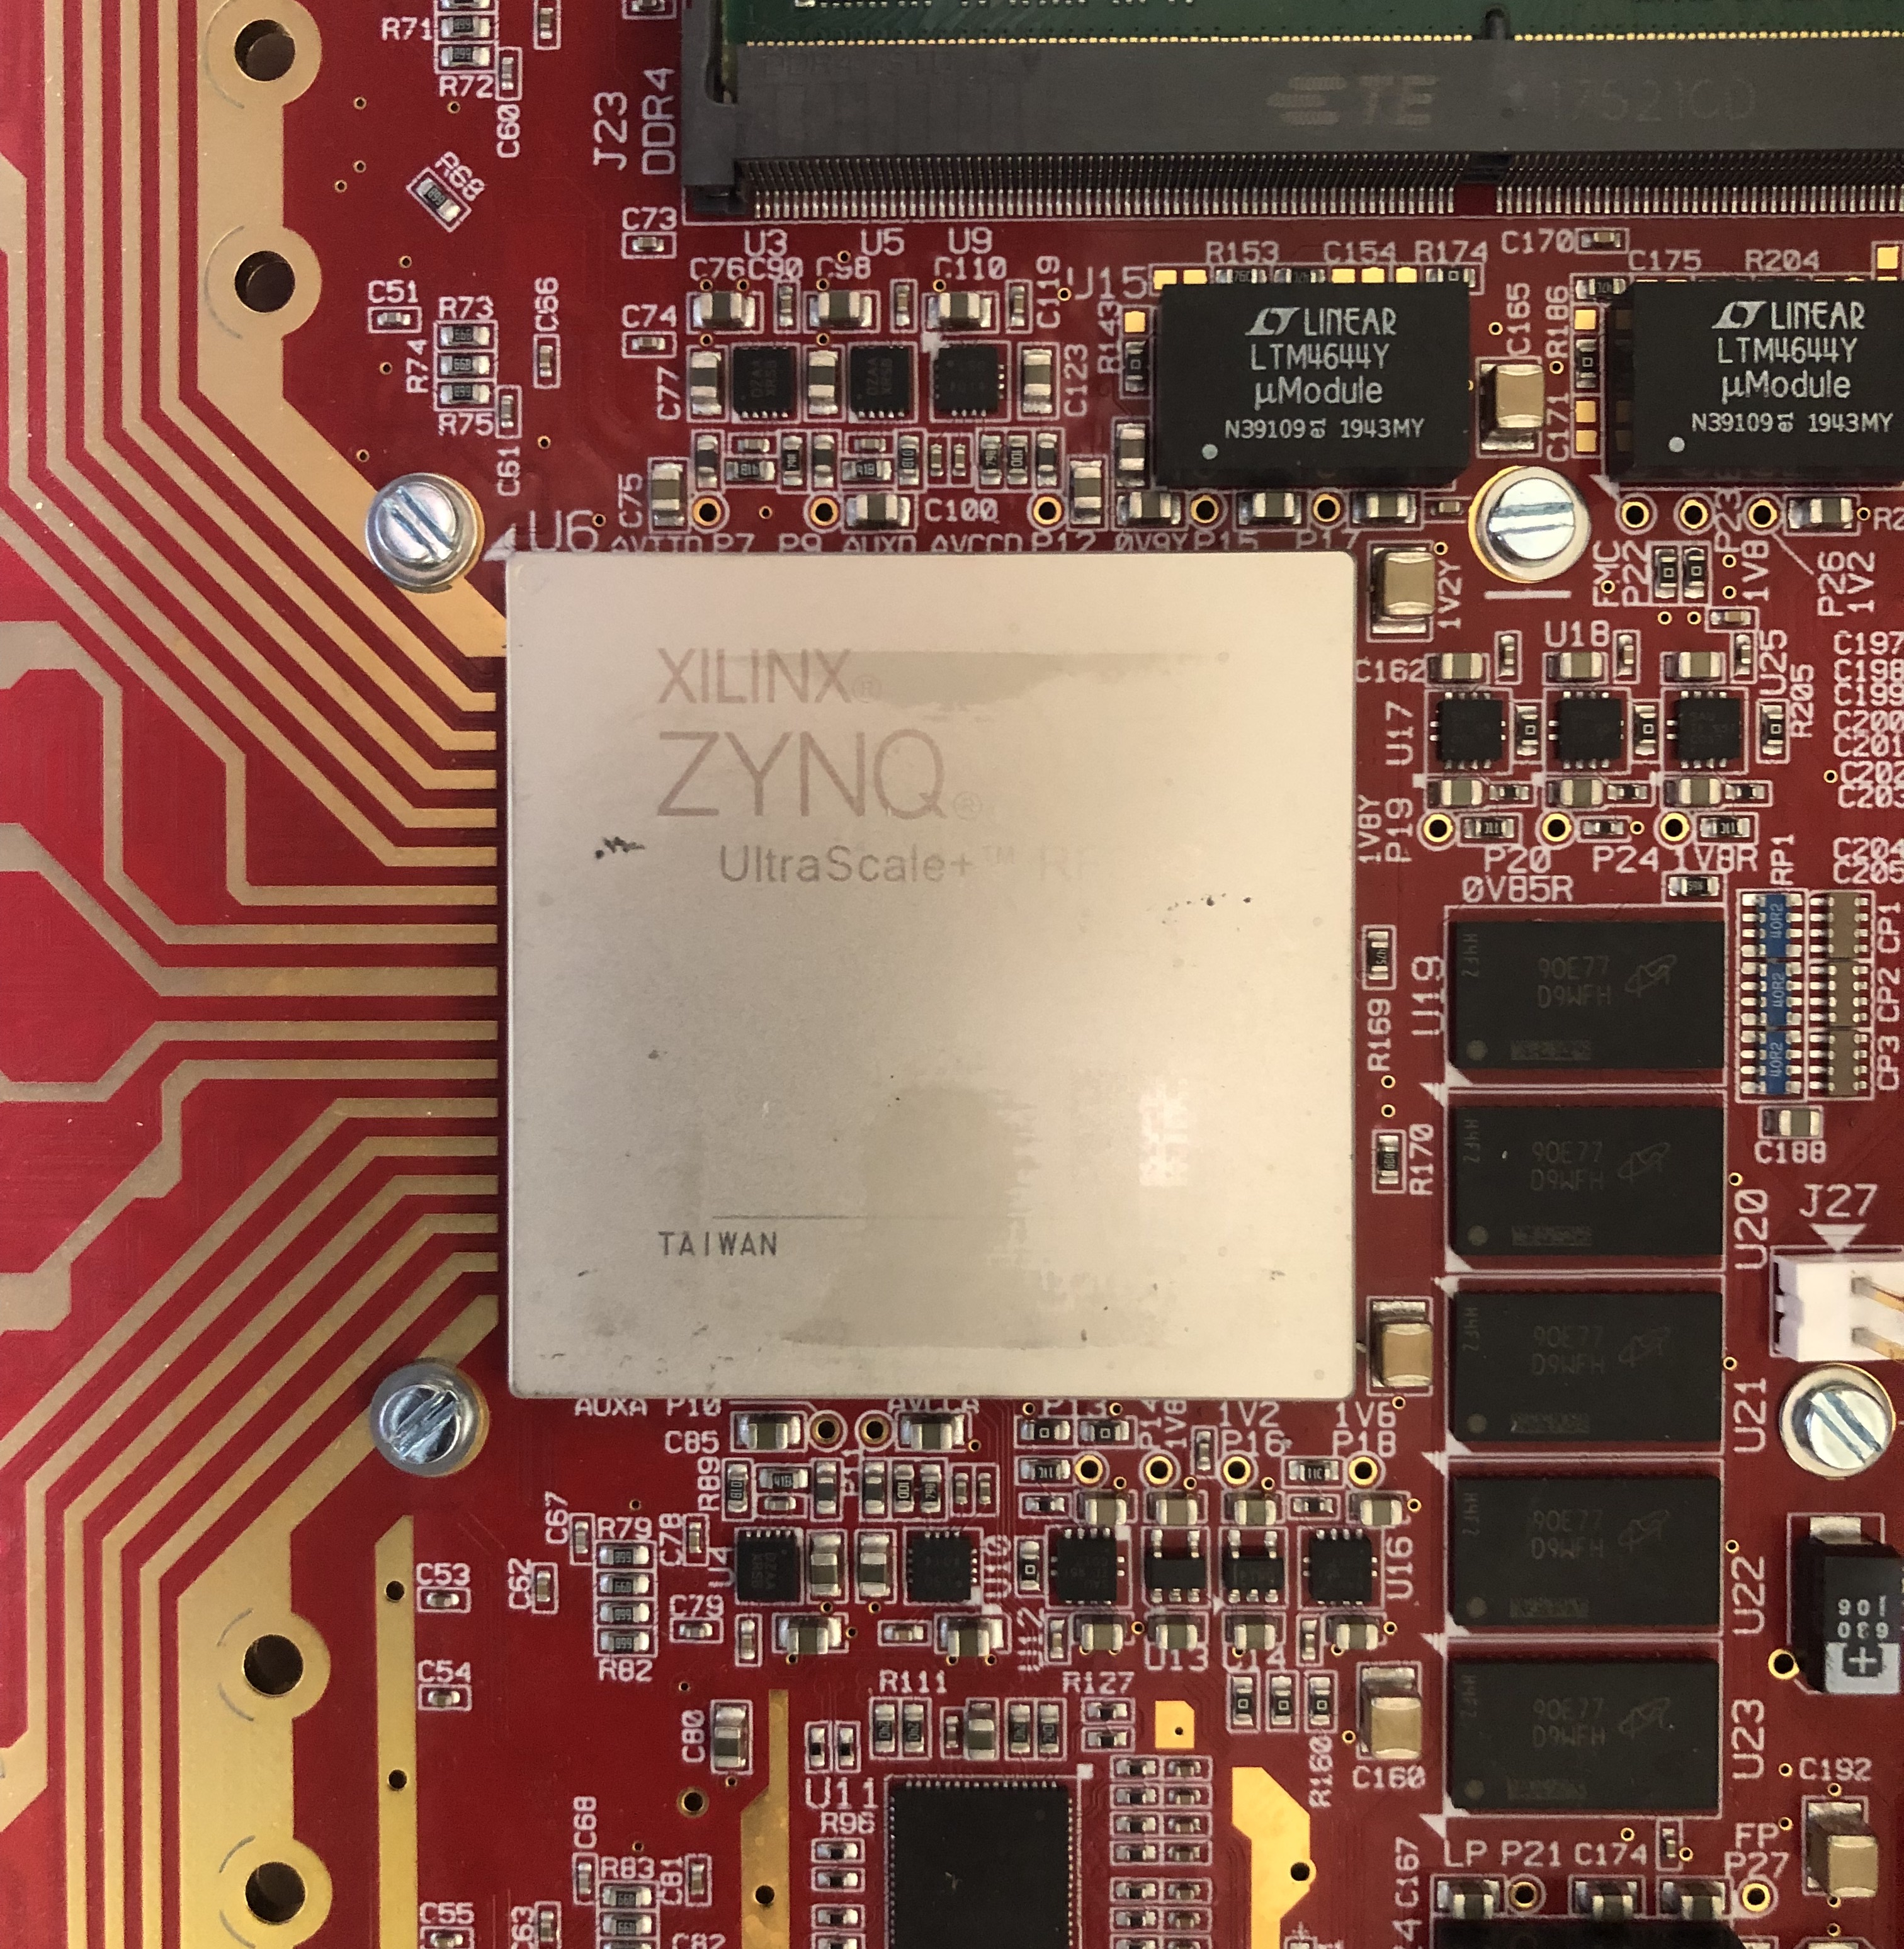
\includegraphics[width=.67\linewidth]{figures/FPGA.jpeg}
\caption{The HTG-ZRF16 Board's FPGA with the HiTech Global Heat Sink Fan Removed}
\label{fig:FPGA}
\end{figure}
%

In place of the HiTech Global heat sink fan, a new heat sink (PN: ATS-55450W-C1-R0) and fan (PN: AFB04512HA) were installed (Figure \ref{fig:New_heat_sink_fan}). This pairing was able to reduce the temperature to $60-65\degree C$ which was deemed acceptable. 

%
\begin{figure}[H]
\centering
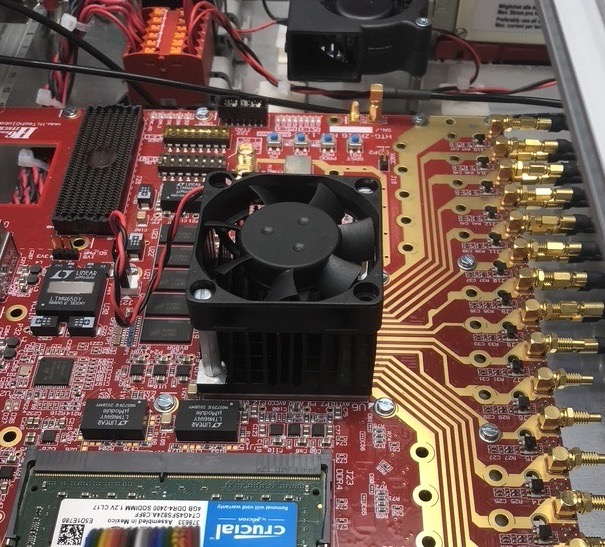
\includegraphics[width=.8\linewidth]{figures/New_heatsink_fan.jpeg}
\caption{The HTG-ZRF16 Board with the New Heat Sink and Fan Installed}
\label{fig:New_heat_sink_fan}
\end{figure}
%

%----------------------------------------------------------------------------------------
%	Interface Board
%--------------------------------------------------------------------------------------

\section{Interface Board}
\label{sec:4}
% ----------------------------------------------------------------

The Interface Board is designed as junction between to the HTG-ZRF16 board and the front panel LEDs which indicate the functionality status of the HTG-ZRF16 board. Assembled in house, Figure \ref{fig:Interface_Board} shows how a completed Interface Board should look. A list of all its required parts appears in Appendix C. 

%
\begin{figure}[H]
\centering
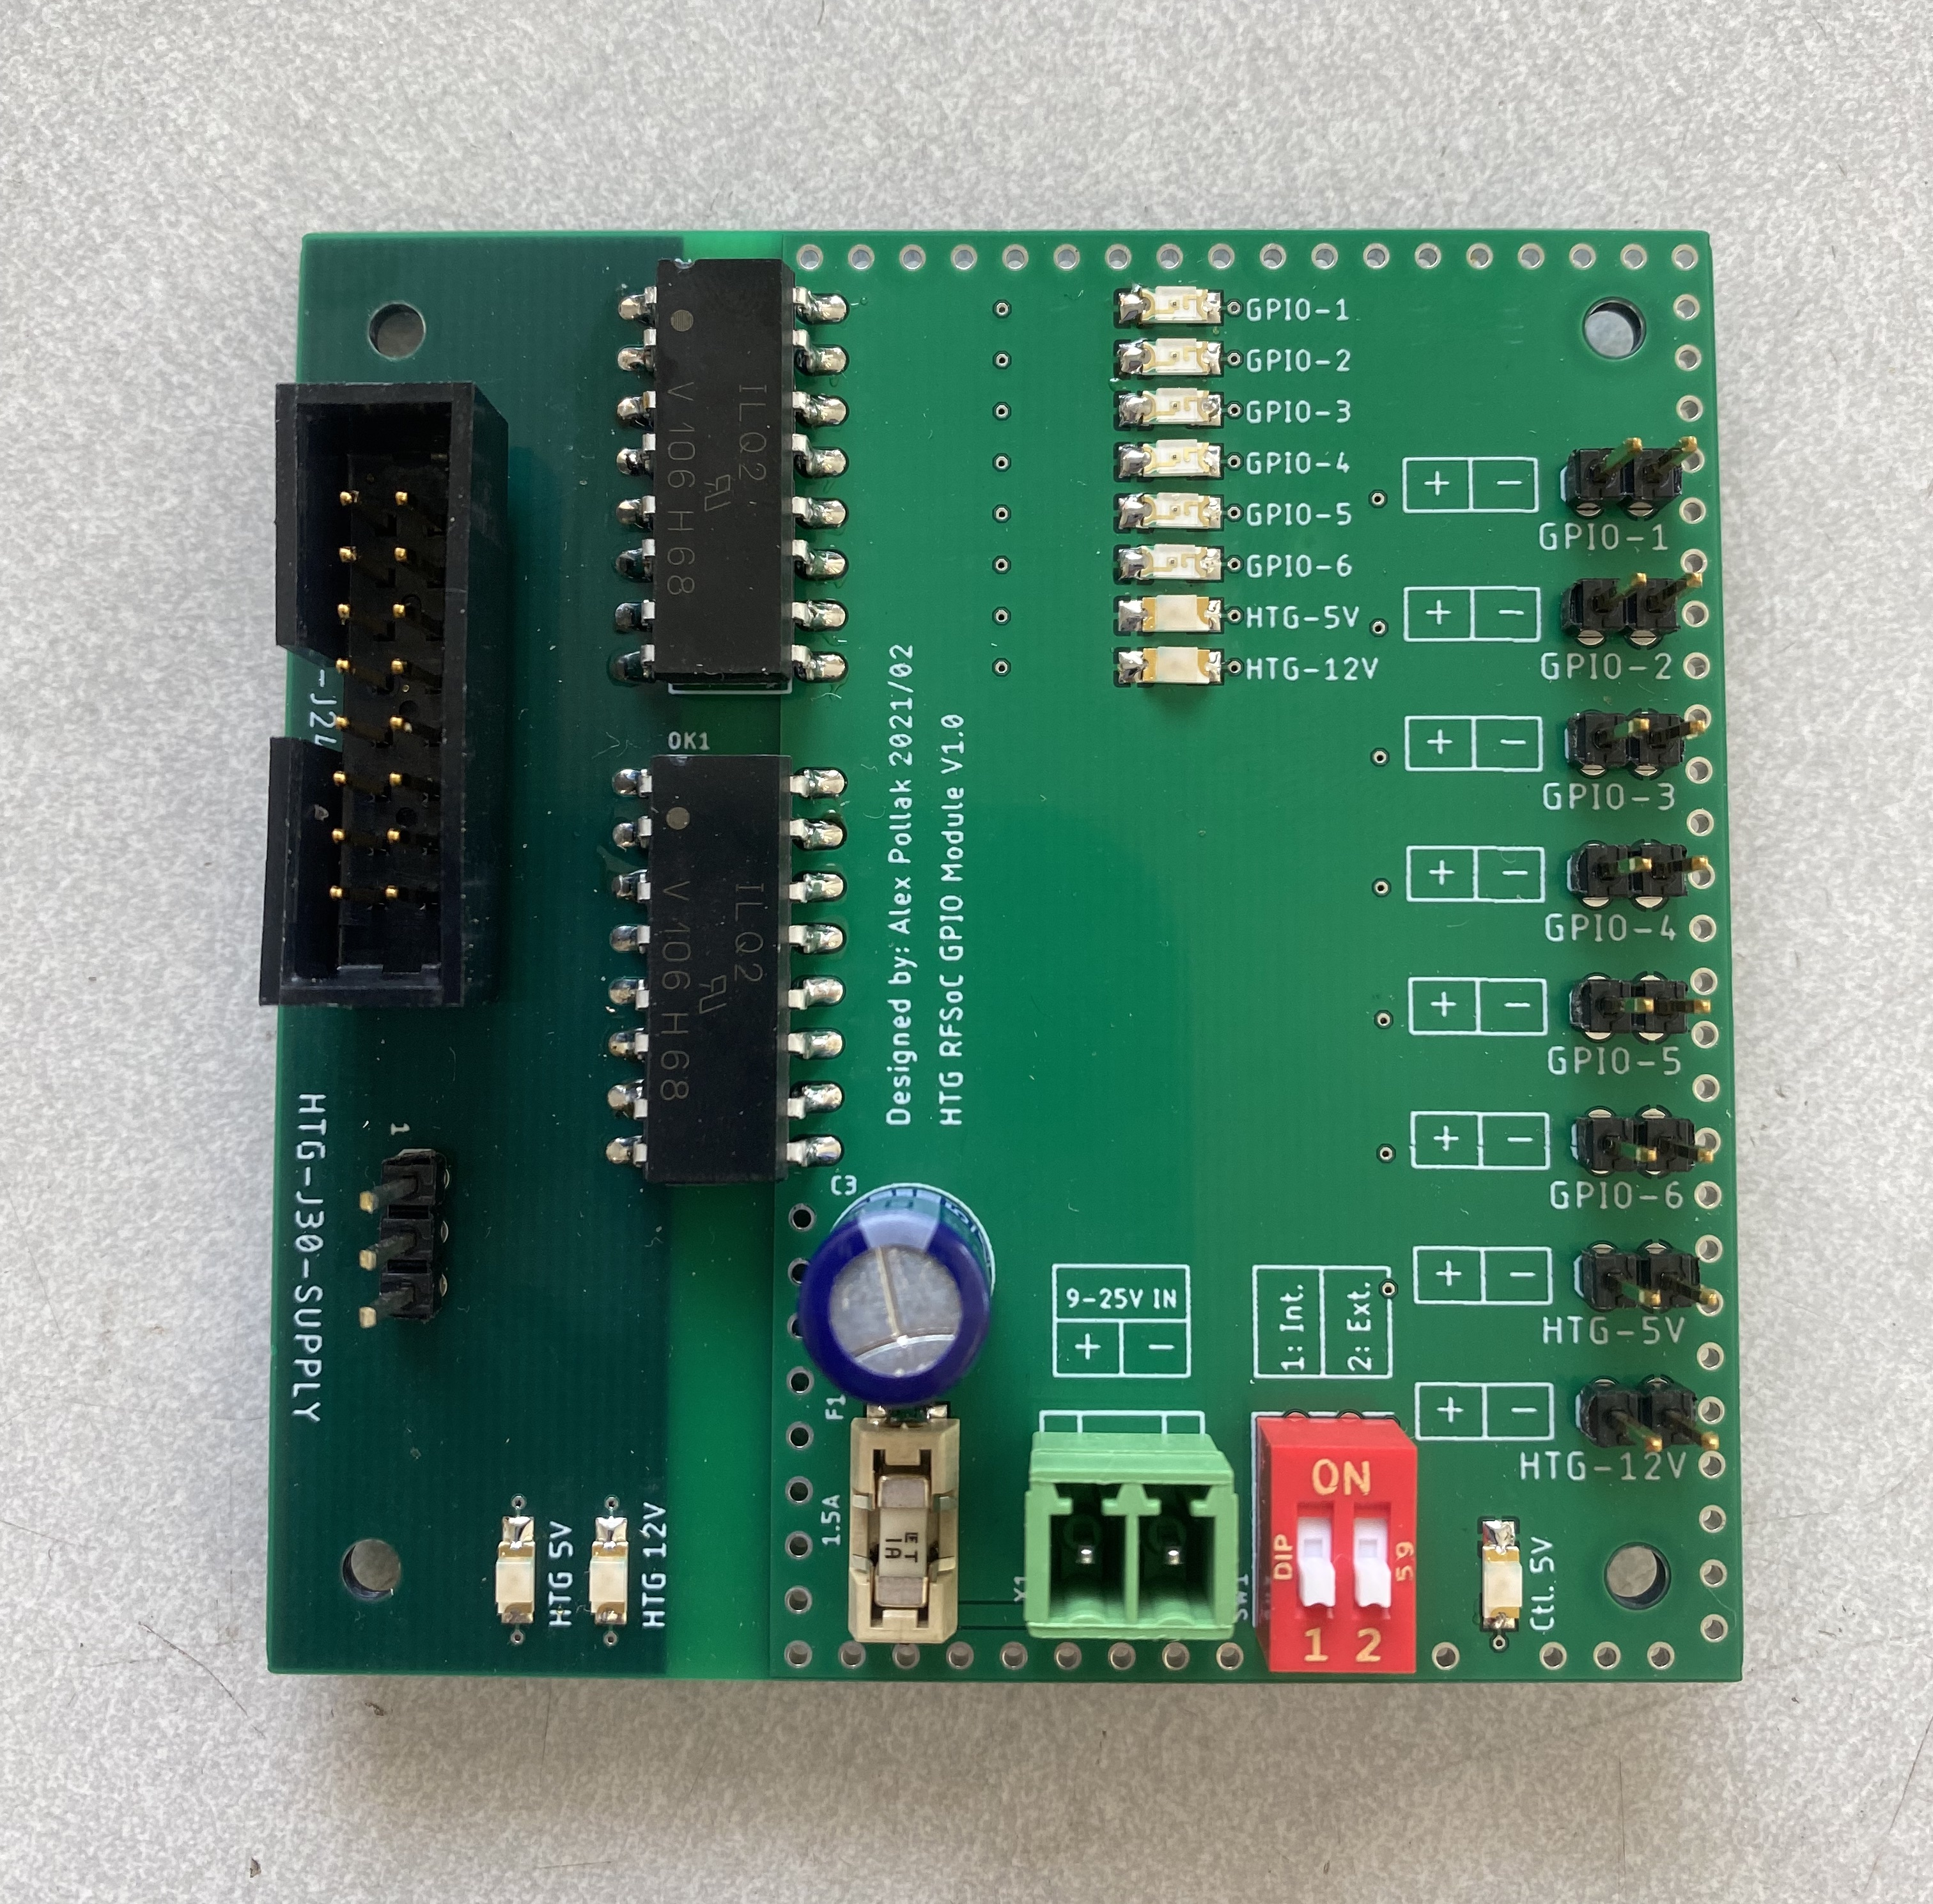
\includegraphics[width=1\linewidth]{figures/Interface_Board.jpeg}
\caption{Completed Interface Board}
\label{fig:Interface_Board}
\end{figure}
%

\subsection{Design}
\label{sec:4.1}
% ----------------------------------------------------------------

The Interface Board electrically isolates any signals from the HTG-ZRF16 board via optocouplers (OK1 and OK2) to avoid any noise contamination. The board is designed to accept 9-25V DC as an input and includes several yellow LEDs (HTG-5V, HTG-12V, HTG 5V, HTG 12V, and Ctl. 5V) that indicate the supply voltage of the HTG-ZRF16 board and Interface Board. Additionally, there are green LEDs (GPIO-1 through GPIO-6) for the HTG-ZRF16 board's GPIOs. Currently, only GPIO 1-3 are used and are set to indicate the HTG-ZRF16 board programming status, the 10 MHz signal, and the 1 PPS signal. Both the green and yellow LEDs are duplicated on the front panel of the module and are connected to the Interface Board via pin-headers. All of these functionalities are reflected in the schematic, Appendix D, and layout, Figure \ref{fig:Interface_Layout}, of the Interface Board. The Interface Board voltage range is 9-25V.

%
\begin{figure}[H]
\centering
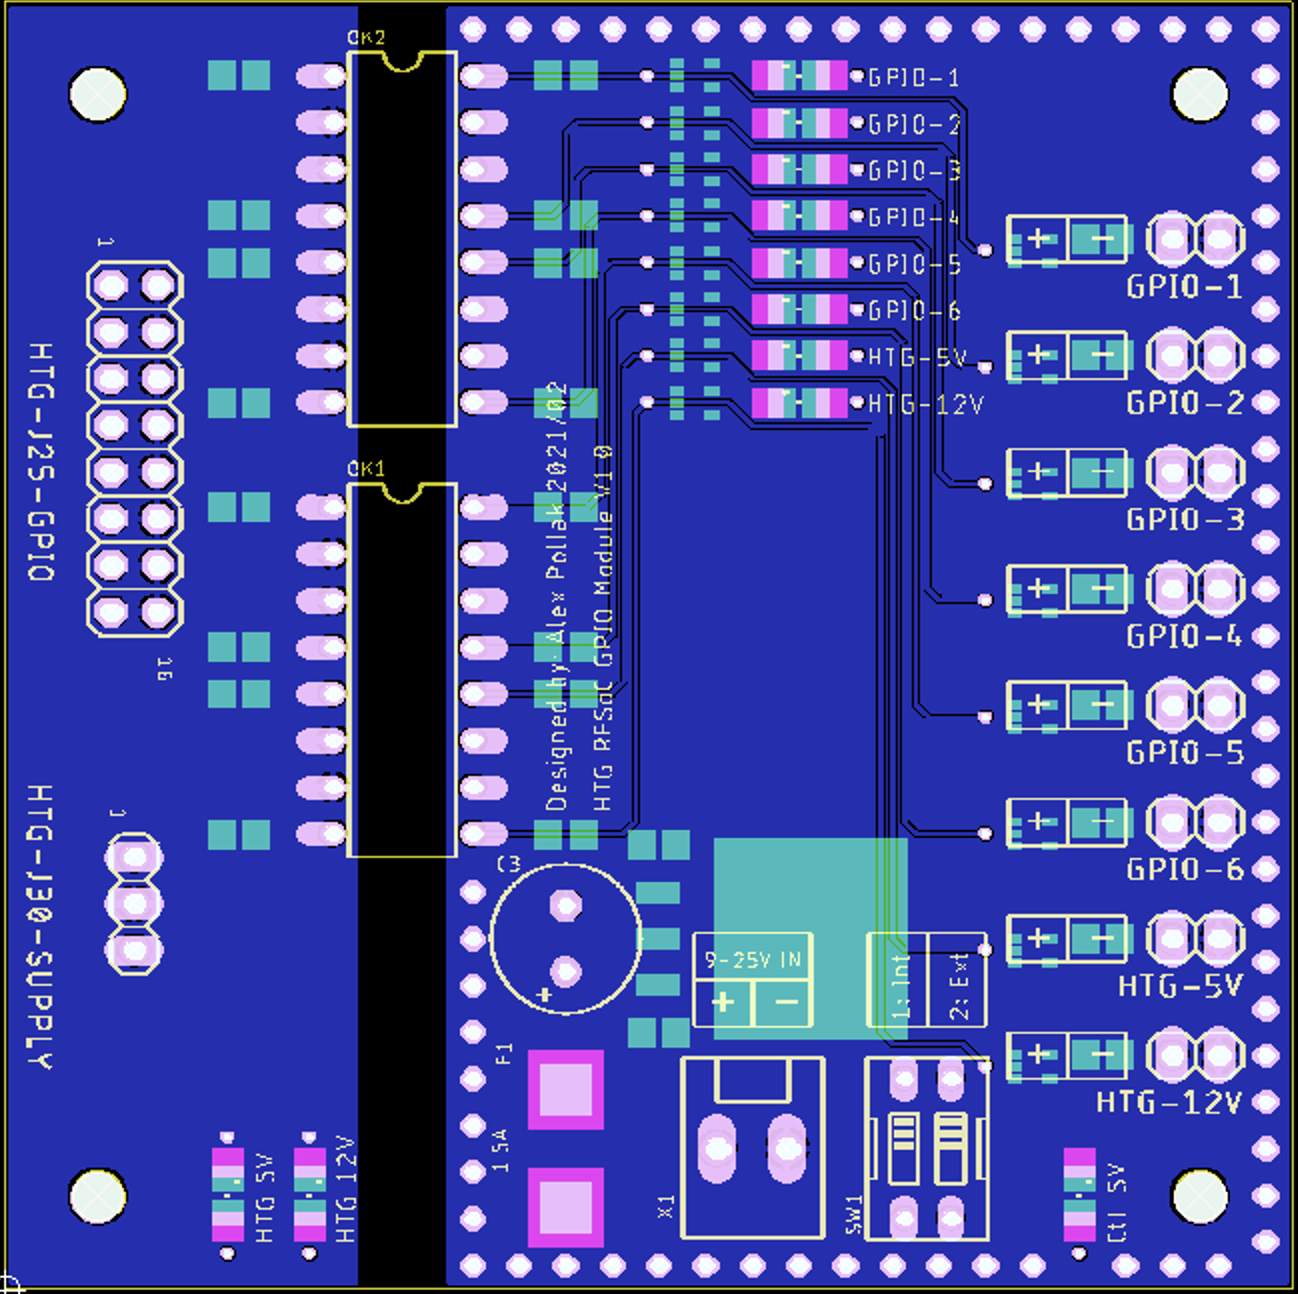
\includegraphics[width=1\linewidth]{figures/Interface_board_layout.png}
\caption{Interface Board Layout}
\label{fig:Interface_Layout}
\end{figure}
%


%----------------------------------------------------------------------------------------
%	Power Supply
%----------------------------------------------------------------------------------------
\section{Power Supply}
\label{sec:5}
% ----------------------------------------------------------------

The module's HTG-ZRF16 board, cooling fans, and the Interface Board are powered with a Schroff Max 180 (PN: 13100-151). The unit is mounted directly to the front panel of the enclosure. The operating temperature range of the power supply is from $-25^{\circ}$C through $85^{\circ}$C, and the technical specifications are shown in Table \ref{tab:psu_spec}. The power entry module (PN: 4304.4005), mounted in the back panel, combines an IEC inlet and a mains filter with a dual-fuse holder. The AC supply fuse current rating for this unit is selected to be 2\,A (PN: 0239002.HXP). 

\begin{table}[H]
\centering
\caption{Power Supply Specification}
\label{tab:psu_spec}
\begin{tabular}{@{}ccccc@{}}
\toprule
\multicolumn{1}{l}{Description} & \multicolumn{1}{l}{Output Voltage} & \multicolumn{1}{l}{Output Current} & \multicolumn{1}{l}{Power W} & \multicolumn{1}{l}{Input Voltage} \\ \midrule
MAX180-112                         & 12\,VDC                               & 13A                               & 156W                         & $100 \sim 240\,\rm{VAC}$                              \\ \bottomrule
\end{tabular}
\end{table}


%----------------------------------------------------------------------------------------
%	Enclosure Wiring
%--------------------------------------------------------------------------------------

\section{Enclosure Wiring}
\label{sec:6}
% ----------------------------------------------------------------

This section outlines the internal connections of the RFSoC Digitizer Module. It is broken up into how parts connect to the front panel, the Interface Board, the HTG-ZRF16 board, the power supply, and the power entry module. Note that there are parts required for wiring the module that do not appear on part lists. This is because they are considered on-hand supplies. These parts include shrink tube, solder, hook up wire, and common terminals.

\subsection{Front \& Back Panel}      
\label{sec:6.1}
% ----------------------------------------------------------------

This section includes the locations of where cables enter the module and connect to the HTG-ZRF16 board within. 



\begin{table}[H]
\caption{Cable Connections for Front Panel}
\centering
\begin{tabular}{@{}ccc@{}}
\toprule
Panel Label & Board Connector Number & Type of Board Connector\\ 
\midrule
IN-1 & J9 & SSMC\\
IN-2 & J10 & SSMC\\
IN-3 & J11 & SSMC\\
IN-4 & J12 & SSMC\\
IN-5 & J13 & SSMC\\
IN-6 & J14 & SSMC\\
IN-7 & J15 & SSMC\\
IN-8 & J16 & SSMC\\
IN-9 & J51 & SSMC\\
IN-10 & J52 & SSMC\\
IN-11 & J53 & SSMC\\
IN-12 & J54 & SSMC\\
IN-13 & J55 & SSMC\\
IN-14 & J56 & SSMC\\
IN-15 & J57 & SSMC\\
IN-16 & J58 & SSMC\\

\bottomrule            
\end{tabular}
\label{table:front_panel}
\end{table}

\begin{table}[H]
\caption{Cable Connections for Back Panel}
\centering
\begin{tabular}{@{}ccc@{}}
\toprule
 Panel Label & Board Connector Number & Type of Board Connector\\ 
\midrule
1 PPS & J17 & MCX\\
10 MHz & J19 & SSMC\\
100 GbE P0 & J35 & QSFP28\\
100 GbE P1 & J34 & QSFP28\\
1 GbE & J37 & RJ45\\

\bottomrule            
\end{tabular}
\label{table:back_panel}
\end{table}

\subsection{Interface Board}
\label{sec:6.2}

The Interface Board is connected to the power supply (PN: 13100-151 ), the HTG-ZRF16 board, and the LEDs (PN: Q6F7BXXB02E).

For the power supply connection, a twisted pair of red and black 18 awg wire was made. Then two E7508 gray ferrules were crimped onto one end and inserted into a 2 Way Cable Mount Screw Terminal (PN: 1803578). This then plugs into the straight PCB terminal block header (PN: 1803426) labeled X1 on the Interface Board.  

The HTG-ZRF16 board is connected to the Interface Board via a a 16 to 16 GPIO Ribbon Cable (PN:IDSD-08-D-06.00) and a twisted triplet of yellow, black, and orange 24 awg wire. The GPIO Ribbon Cable provides the status of GPIO's 1-3 to the green LEDs while the twisted triplet provides the status of power to the HTG-ZRF16 board (HTG 5V and 12V) to the yellow LEDs. The GPIO Ribbon Cable plugs into HTG-J25-GPIO on the Interface Board and J25 on the HTG-ZRF16 board. The twisted triplet was crimped with M20 Crimp Terminals (PN:M20-1180042) which were then inserted into a 3 Pin SIL Housing (PN: M20-1060300). The twisted triplet plugs into HTG-J30-Supply on the Interface Board and J30 on the HTG-ZRF16 board. See Figure \ref{fig:power_indicator_cable} for how the triple if orientated on each board. 

\begin{figure}[H]
\centering
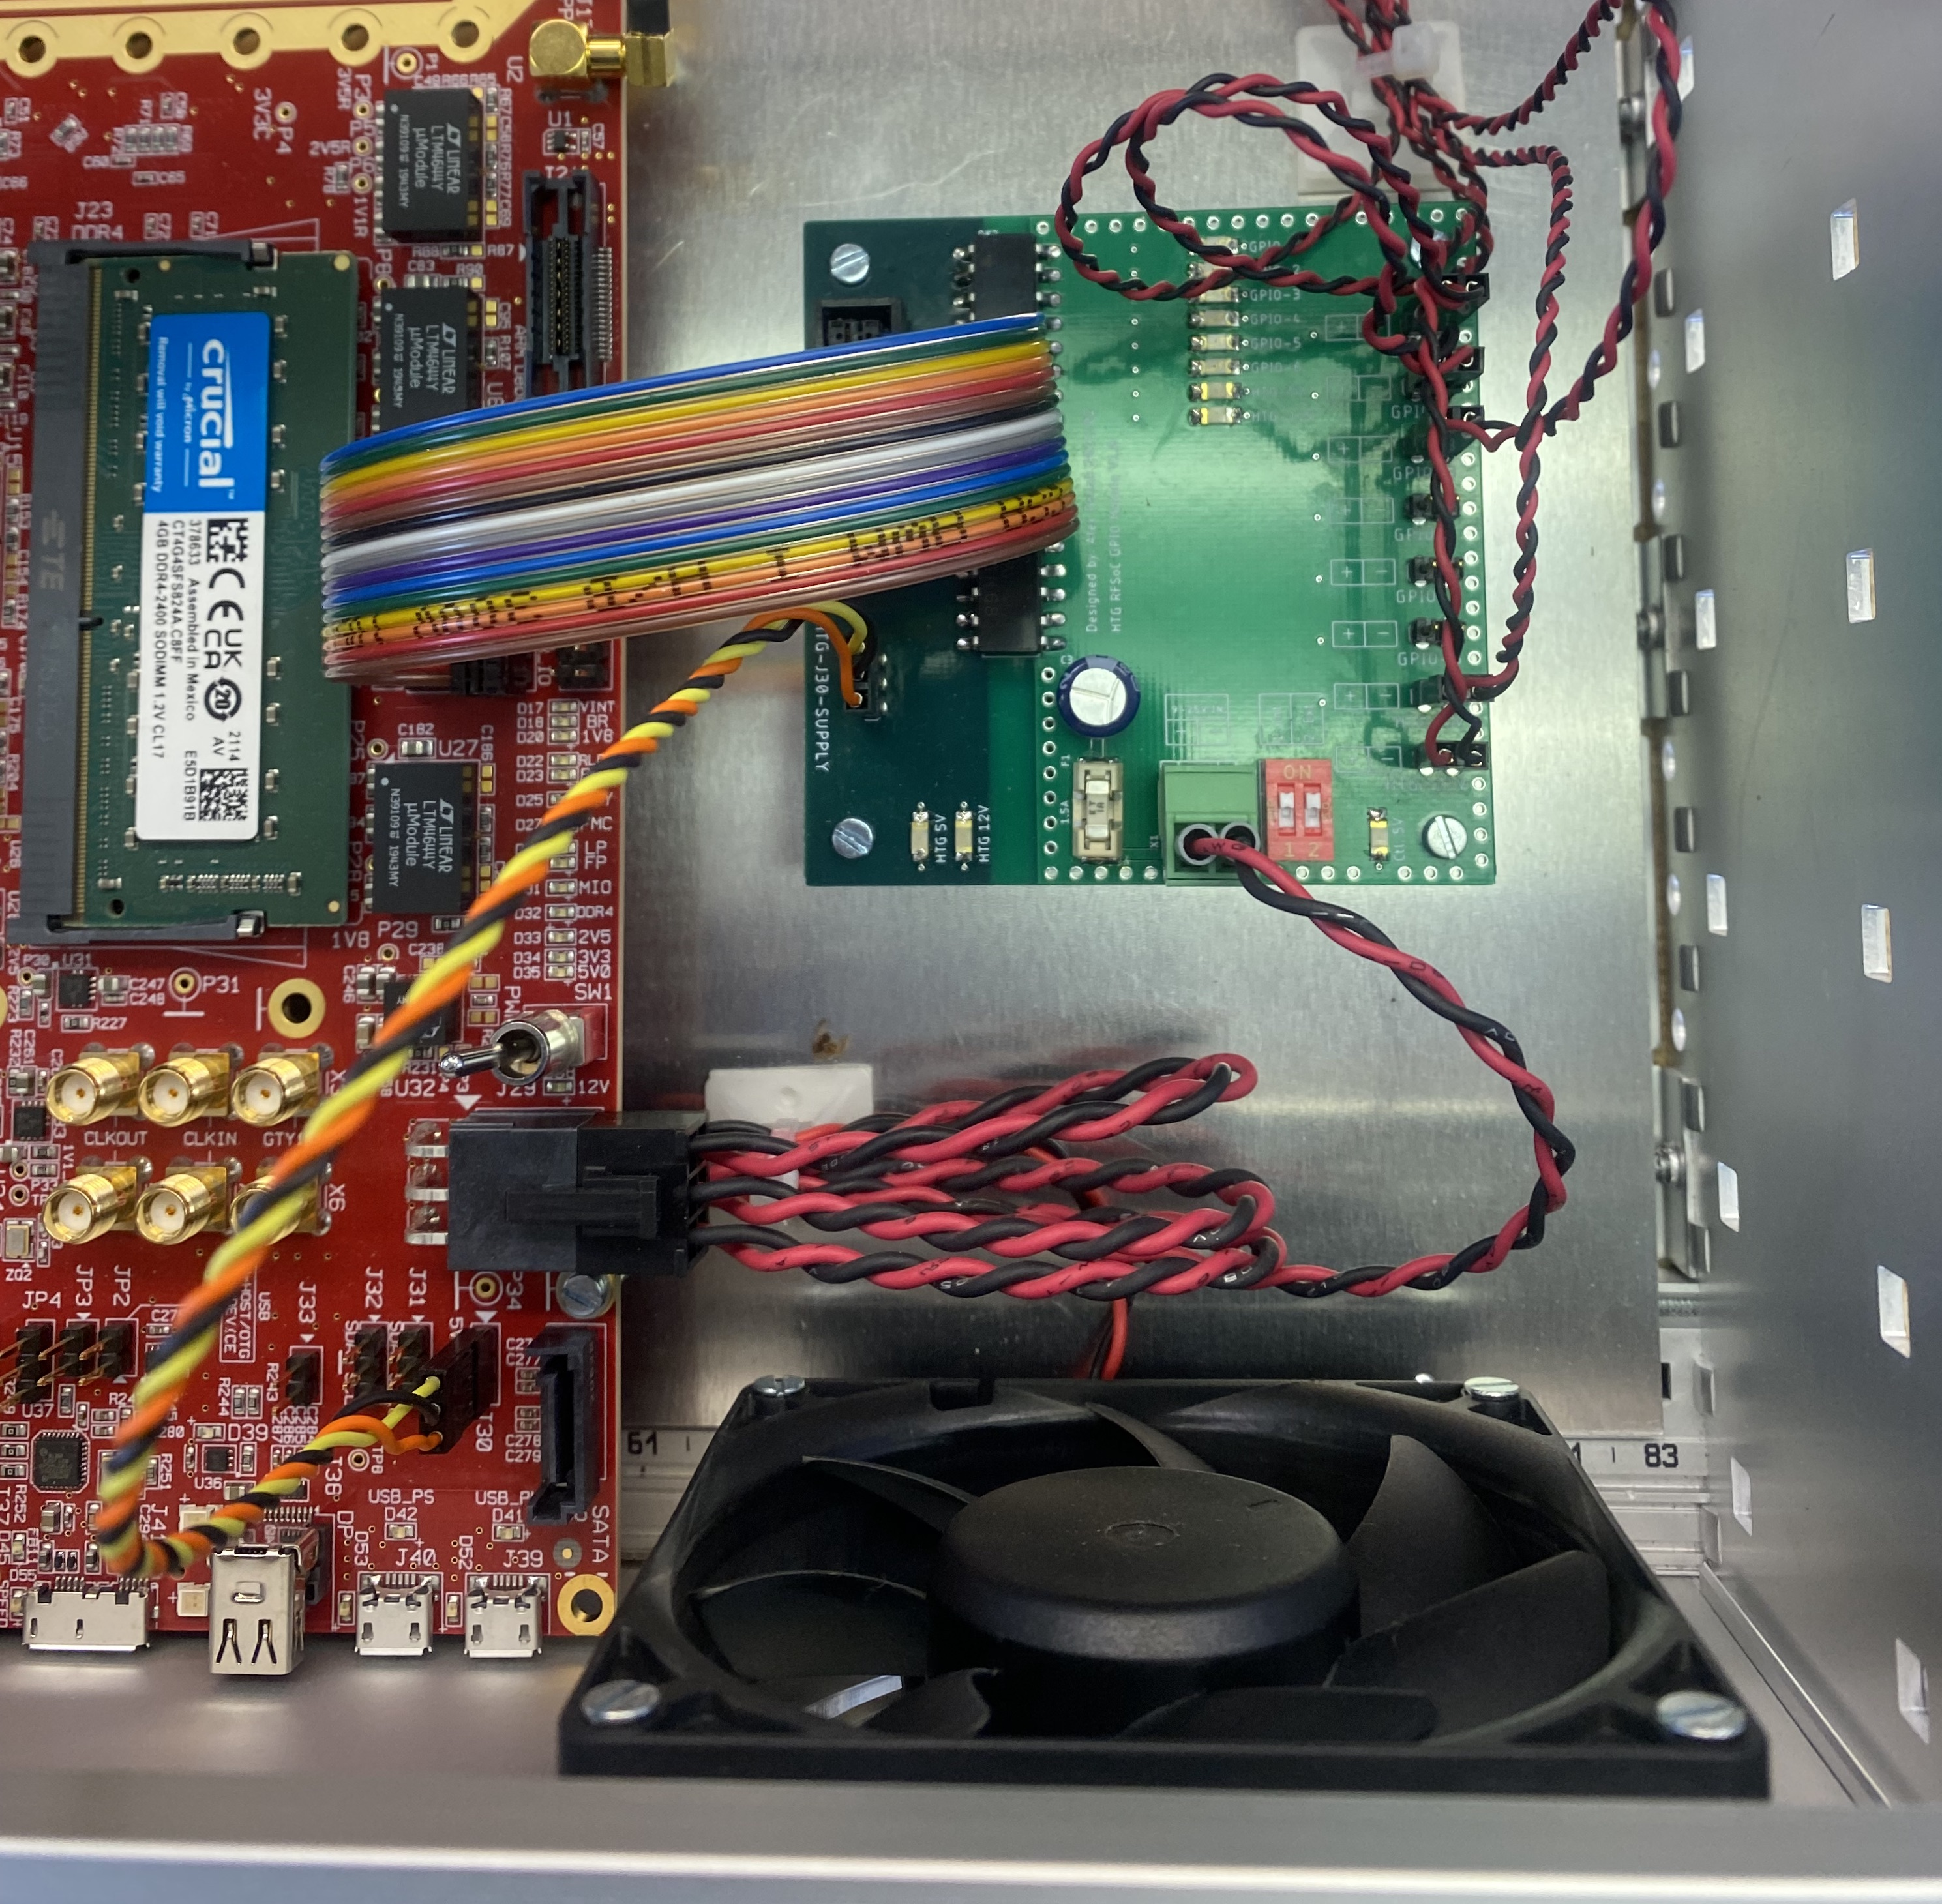
\includegraphics[width=1\linewidth]{figures/Power_indicator_cable.jpeg}
\caption{HTG-ZRF16 and Interface Board's Cable Orientations}
\label{fig:power_indicator_cable}
\end{figure}

The five LEDs' wires are extended with red and black 28 awg as to reach the Interface Board. They are then crimped with M20 Crimp Terminals which are inserted into a 2 Pin SIL Housing (PN: M20-1060200). The Interface Board has eight two pin Straight PCB Headers (PN: 42375-2486), five of which the LEDs plug into. Table \ref{LED_to_board} shows which LEDs plug into which headers on the board. 

\begin{table}[H]
\caption{LED Internal Cable Connections}
\centering
\label{LED_to_board}
\begin{tabular}{@{}cc@{}}
\toprule
 LED Panel Label & Board Connector Label\\ 
\midrule
12V & HTG-12V\\
5V & HTG-5V\\
Prog. & GPIO-1\\
10 MHz & GPIO-2\\
1 PPS & GPIO-3\\

\bottomrule            
\end{tabular}
\label{table:LED_to_board}
\end{table}

% ----------------------------------------------------------------

\subsection{HTG-ZRF16 Board}
\label{sec:6.3}

The HTG-ZRF16 board connects to the power supply (PN: 13100-151), Interface Board, the heat sink fan (PN: AFB04512HA), front panel, and back panel.

The power supply is connected to the HTG-ZRF16 board via six wires, three red for 12V and three black for ground. The six wires are 18 awg and are twisted into pairs. Each wire is crimped with a Minifit plus terminal (PN: 45750-1112) and then all six are plugged into a Molex Minifit Jr. 6 Socket Receptacle (PN: 45559-0002) as shown in Figure \ref{fig:board-power}. Before installation, check the polarity. Figure \ref{fig:power_indicator_cable} shows how the cable looks once completed and how it should be orientated. 


\begin{figure}[H]
\centering
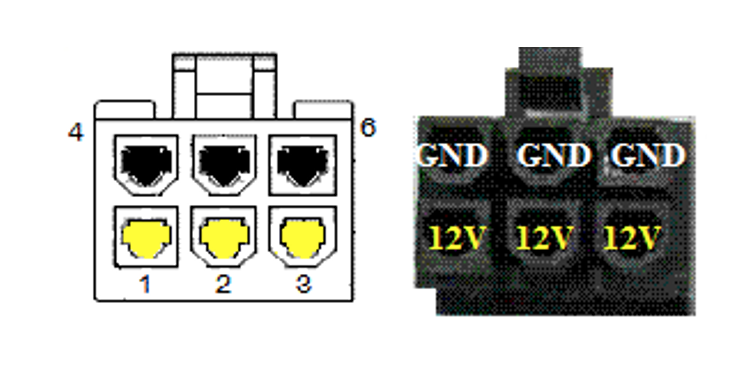
\includegraphics[width=1\linewidth]{figures/6pin 12V.png}
\caption{The Molex board power adapter}
\label{fig:board-power}
\end{figure}

The Interface Board connections to the HTG-ZRF16 board are outlined in the Interface Board section above. 

As noted in the Section \ref{sec:4}, the HTG-ZRF16 board has a heat sink fan due to high temperature while in use. This heat sink fan is connected directly to the board for power via J27. Though, prior to being plugged in, the fan's wires are twisted together, crimped with M20 Crimp Terminals (PN:M20-1180042), and inserted into a 2 Pin SIL Housing (PN: M20-1060200). 

The front and back panel connections to the HTG-ZRF16 board are outlined in Table \ref{table:front_panel} and \ref{table:back_panel}. The 100 GbE P0, 100 GbE p1, and 1 GbE connections from the back panel plug directly from the back panel into the HTG-ZRF16 board. The rest of the back panel connections and all the front panel connections are done via SMA Female Bulkhead to SSMC Plug Cables (PN: PE3C4448-18),

% ----------------------------------------------------------------

\subsection{The Fans}
\label{sec: the 6.4}

There are a total of ten fans inside the RFSoC Digitizer Module. The first of these is the heat sink fan (PN: AFB04512HA) which was already discussed in the previous section. The rest of the fans are connected to the power supply. There is the front panel fan (PN: PF80251V1-1000U-A99), the back panel fan (PN: PF80251V1-1000U-A99), the blower fan (PN: GB1205PKV1-8AY.GN), and six base plate fans (PN: 412FM). The front panel and back panel fans wires are extended with red and black 20 awg in order to reach the power supply. The blower fan's wires are long enough as is, and the six base plate fans' wires are soldered together and extended with and red and black 20 awg wires. 

Regarding how the fans should be mounted, the front panel fan should blow air into the enclosure while the back panel to sucks air out of the enclosure. The six base plate fans should be mounted such that they blow air into the enclosure. The front panel, back panel, and blower fan can all be seen in Figures \ref{fig:CAD-Iso} and \ref{fig:CAD-top}. However, the six base plate fans are not visible, nor can they be seen in the completed enclosure (Figures \ref{fig:Enclosure_above} through \ref{fig:Enclosure_in_Rack}). Figure \ref{fig:six_fan_front} and \ref{fig:six_fan_back}, instead, shows an incomplete RFSoC Digitizer Module with the six base plate fans visible.

\begin{figure}[H]
\centering
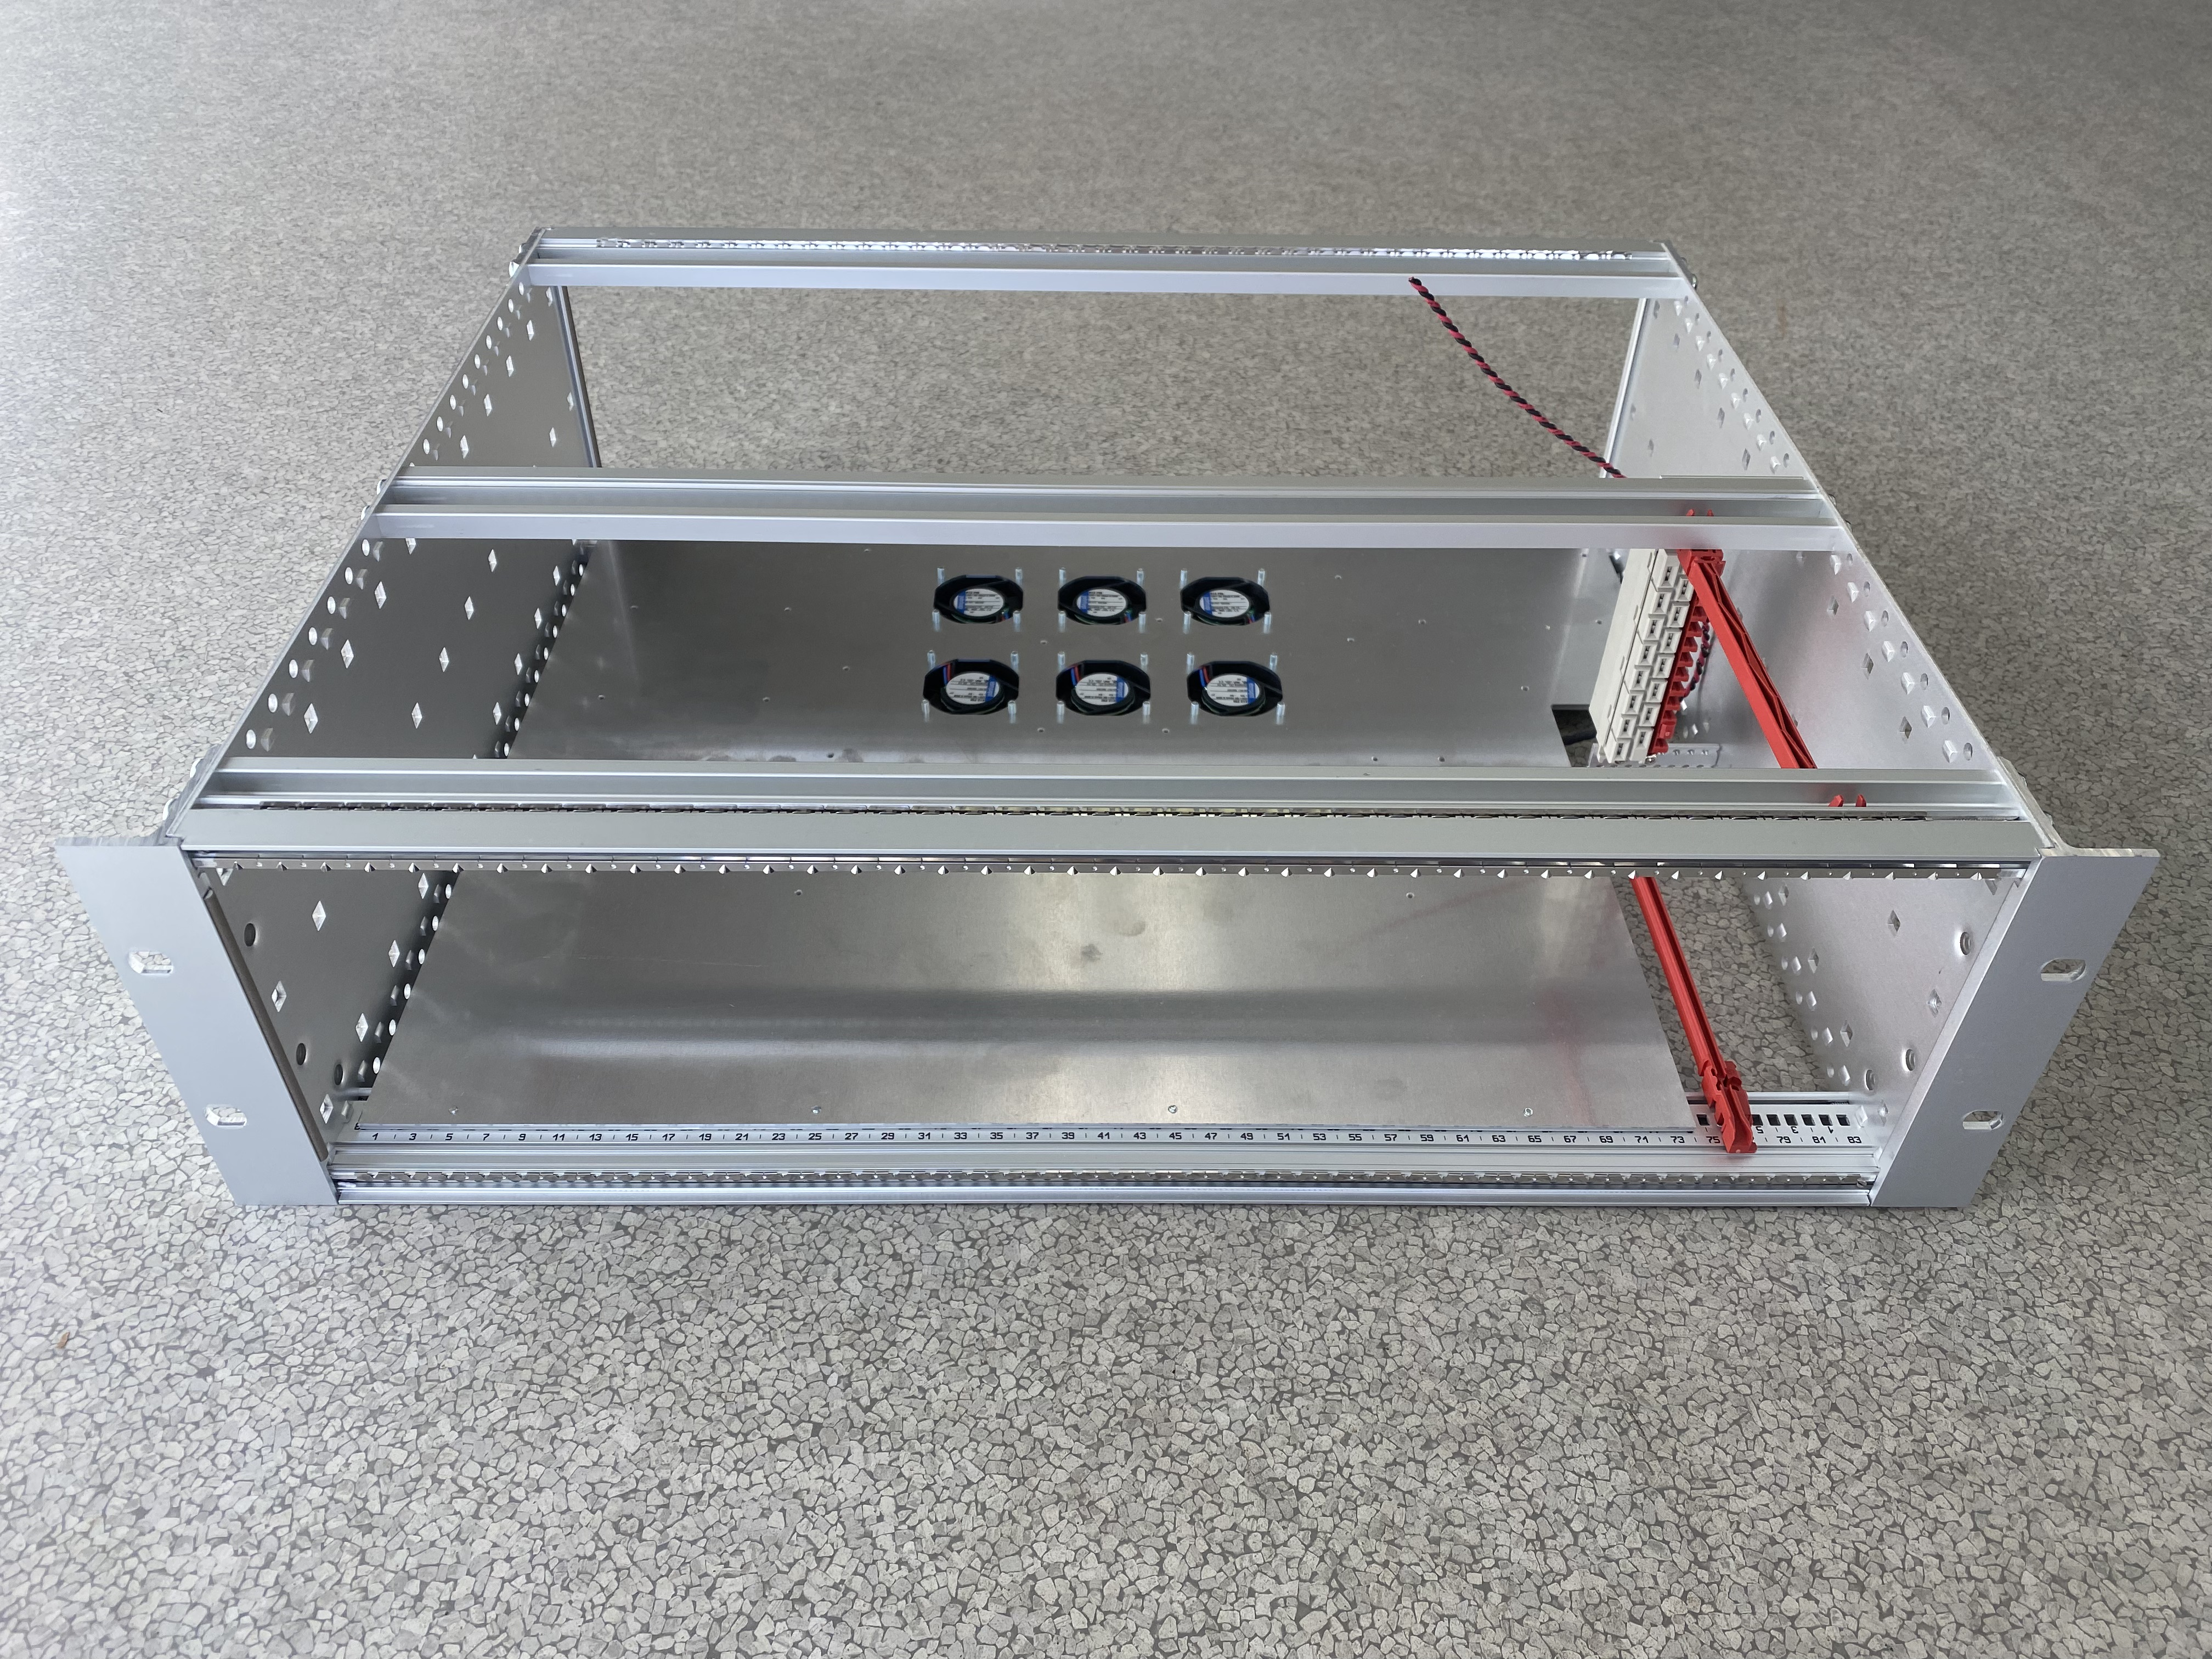
\includegraphics[width=1\linewidth]{figures/Six_Fan_Front.jpeg}
\caption{Front view of an incomplete RFSoC Digitizer Module}
\label{fig:six_fan_front}
\end{figure}

\begin{figure}[H]
\centering
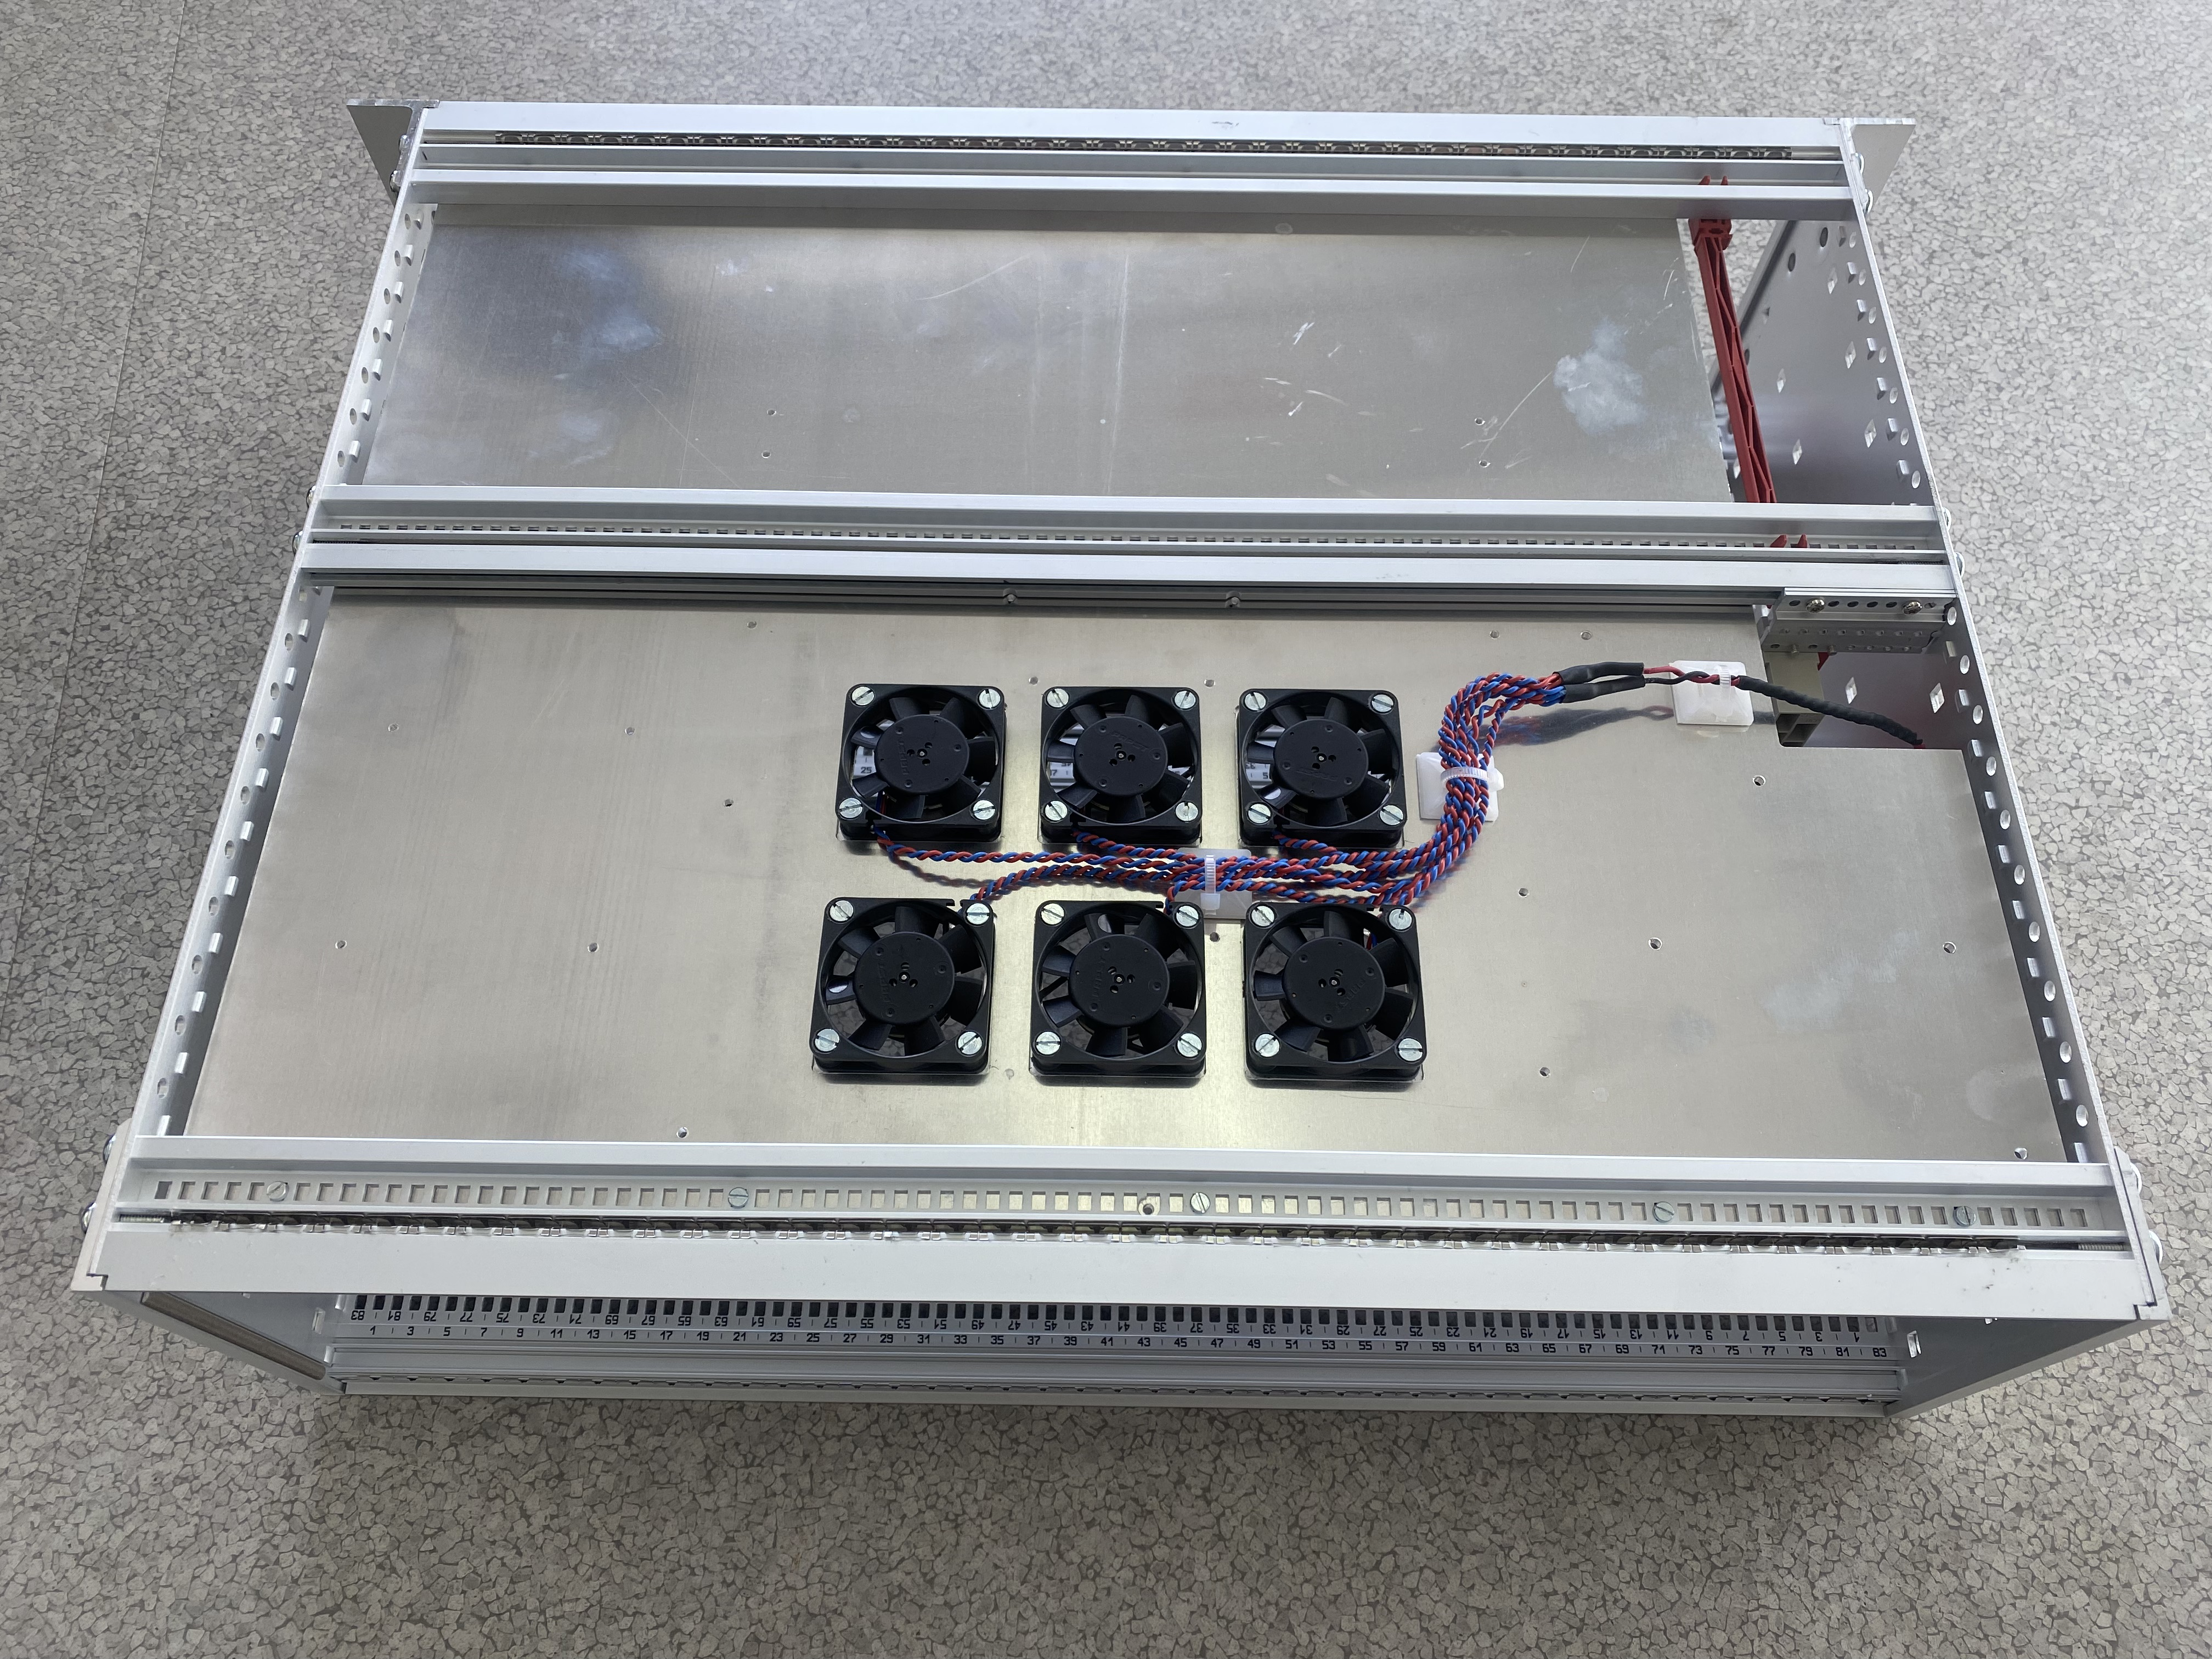
\includegraphics[width=1\linewidth]{figures/Six_Fan_Back.jpeg}
\caption{Back and upside down view of an incomplete RFSoC Digitizer Module}
\label{fig:six_fan_back}
\end{figure}

% ----------------------------------------------------------------

\subsection{Power Supply}
\label{sec: the 6.5}

The power supply (PN: 13100-151) is connected to the Interface Board, the HTG-ZRF16 board, the fans, and the power entry module (PN: 4304.4005). 

Due to the large number of components requiring power, the power supply uses a set of power distribution terminals (PN: 3273158 and 3273168) shown in Figure \ref{fig:Power_Distribution Terminals}. Please see Figure \ref{fig:RFSoC_Power_Schematic_1} for a schematic that shows how the power supply is connected to the power distribution terminals. The red and black wires used are 14 awg and are both crimped with female quick disconnect terminals (PN: FDFD1-250) on the ends plugging into the power supply. The ends plugging into the power distribution terminal are just stripped. There is also a green ground wire that connects the black power distribution module to the base plate. This wire is stripped on the power distribution terminal end and crimped with a 6s eye terminal on the other. The eye terminal is screwed down to the base plate.

\begin{figure}[H]
\centering
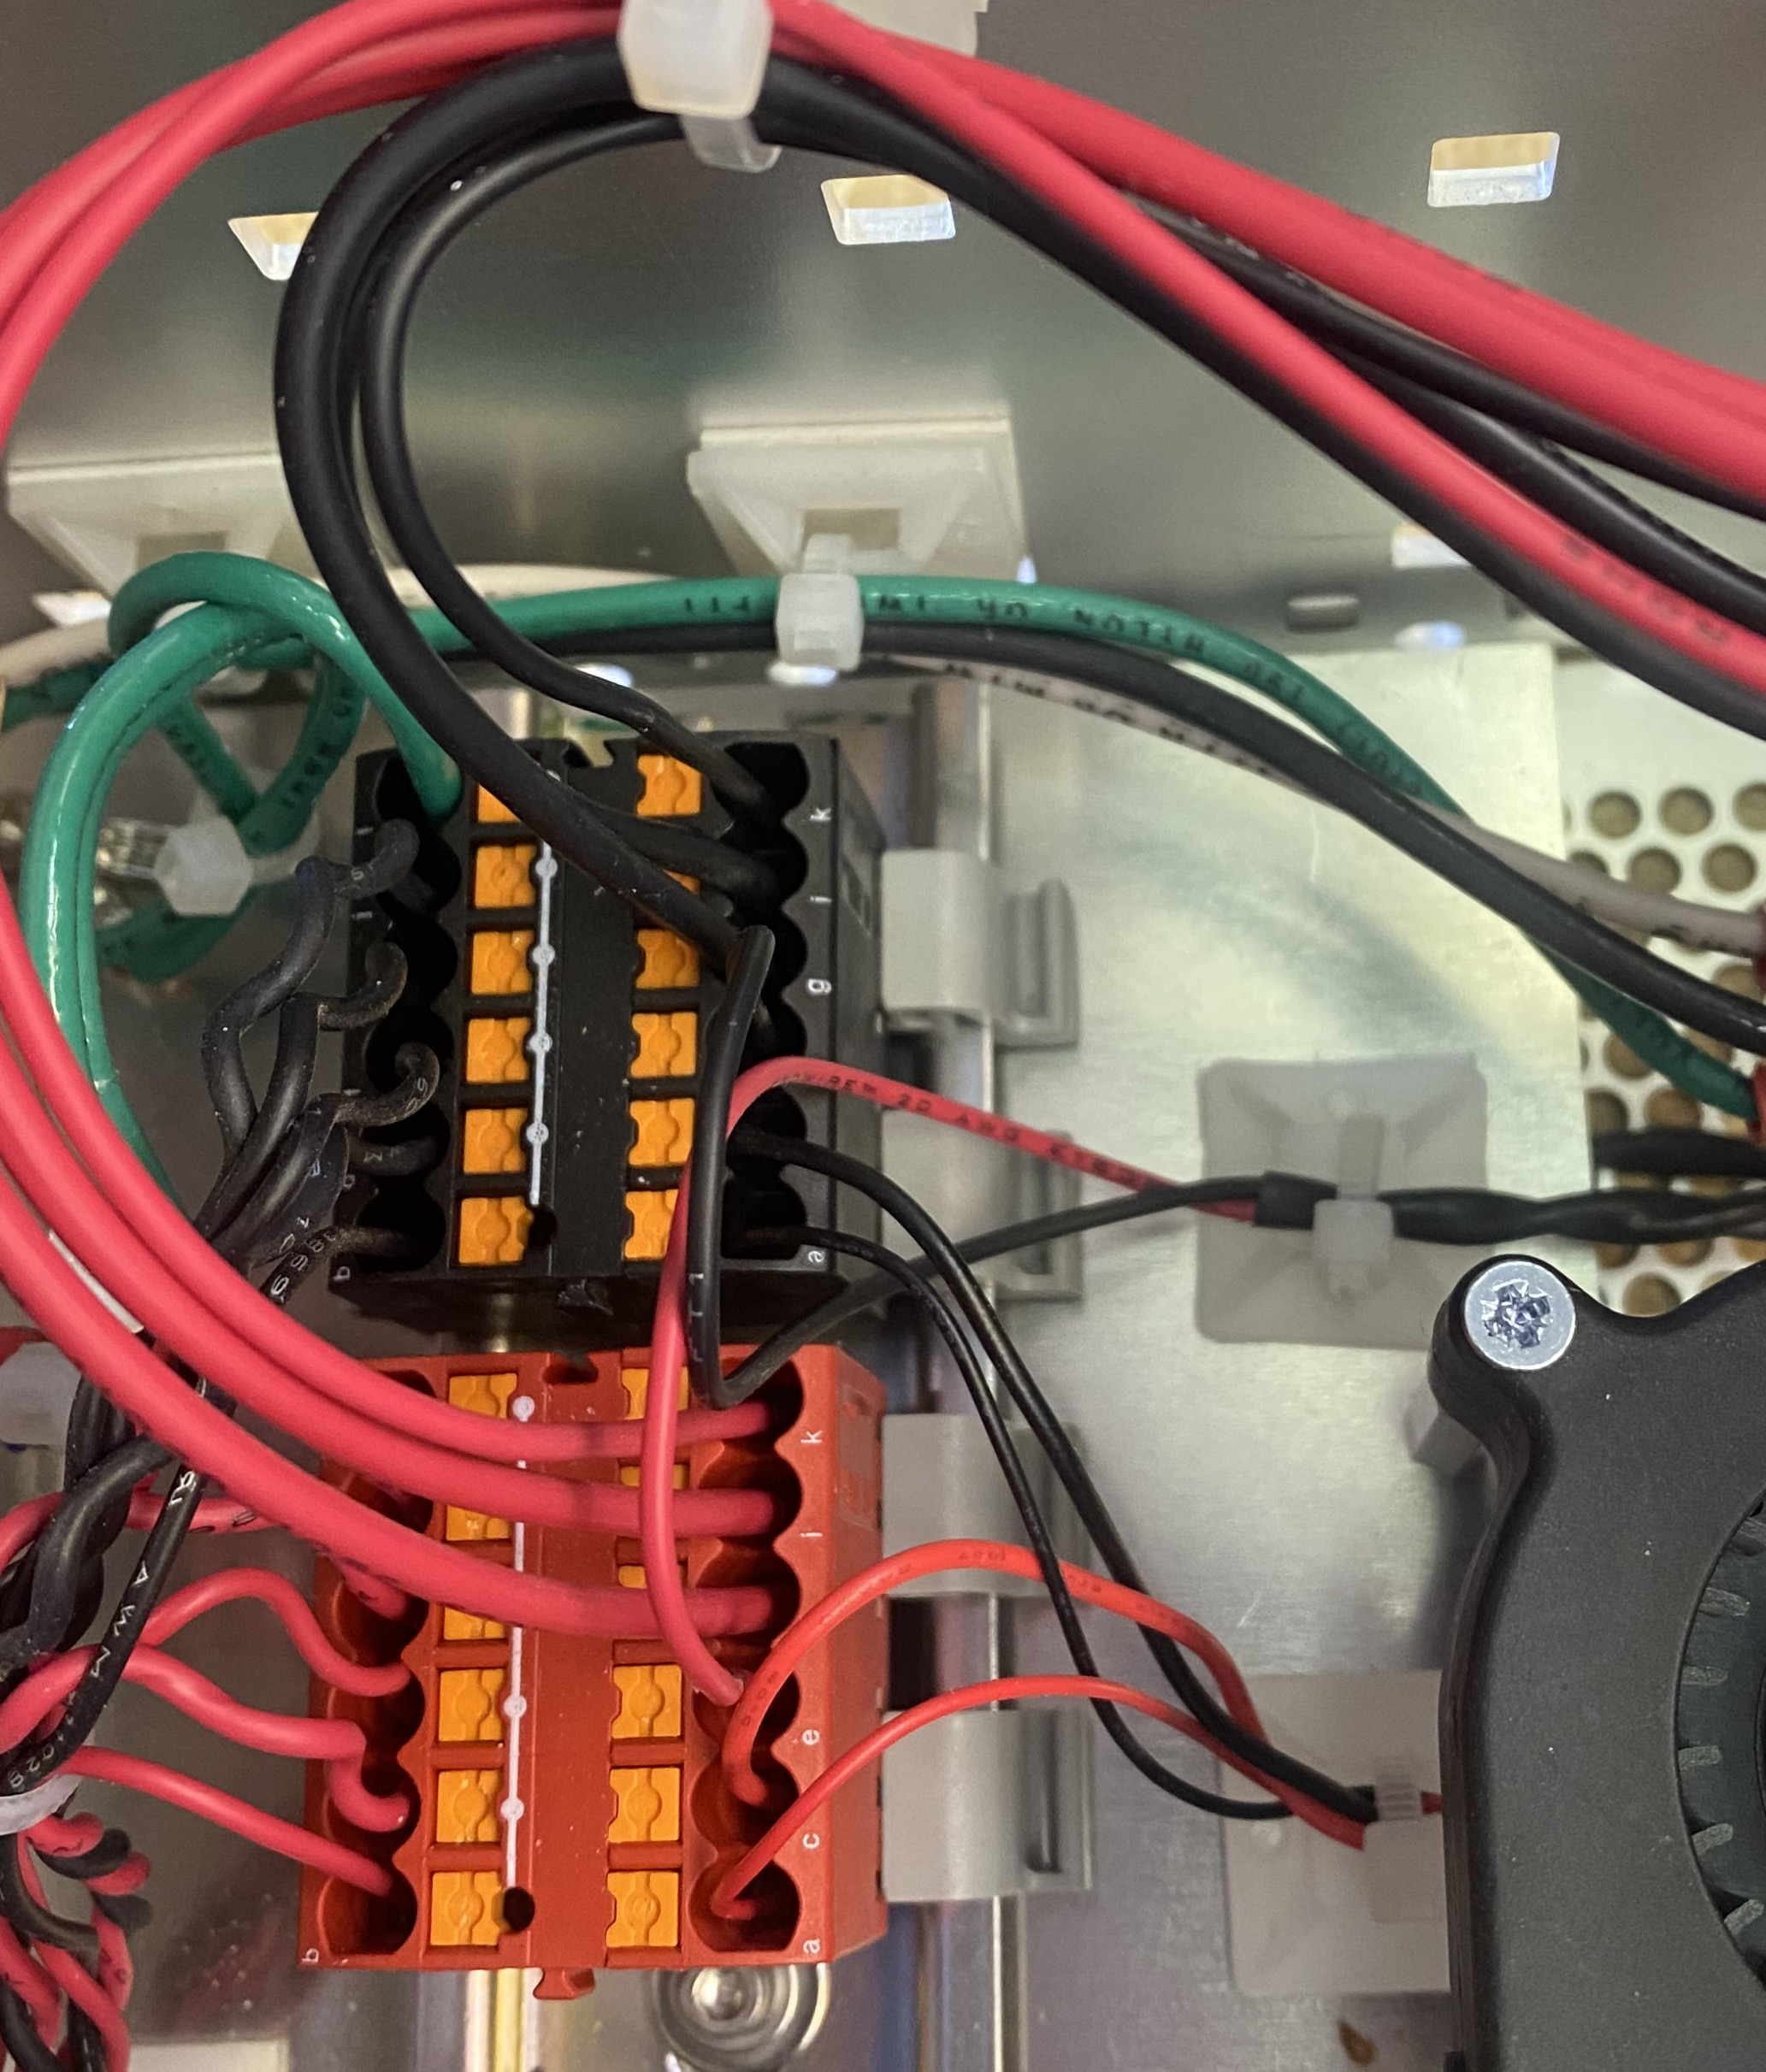
\includegraphics[width=.8\linewidth]{figures/Power_Distribution_Terminals.jpeg}
\caption{The Power Distribution Terminals Installed in the RFSoC Digitizer Module}
\label{fig:Power_Distribution Terminals}
\end{figure}

A schematic of how the power distribution terminals are connected to the Interface Board, the HTG-ZRF16 board, and the fans is shown in Figure \ref{fig:RFSoC_Power_Schematic_2}. See the above sections for wires gauges, terminals, and housings used for all these connections. 

How the power supply is connected to the power entry module is shown in Figure \ref{fig:RFSoC_Power_Schematic_1}. The black and white wires are crimped on both ends with female quick disconnect terminals. The green ground wire for the power supply has female quick disconnect terminals on both ends as well, and rather than being connected directly to the base plate, it instead plugs into the female piggyback disconnect terminal (PN:
PBDD2-250) of the power entry module's ground wire. 

\begin{figure}[H]
\centering
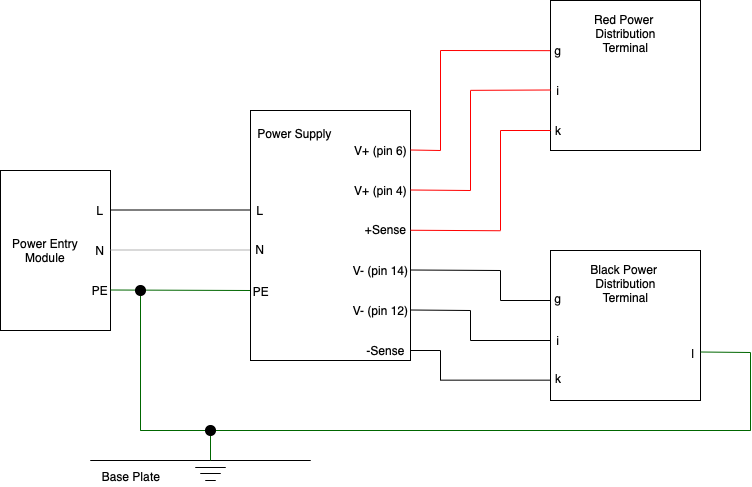
\includegraphics[width=1\linewidth]{figures/RFSoC_Power_Schematic_1.png}
\caption{RFSoC Digitizer Module Power Schematic Part 1. This half of the power schematic shows the connections between the power entry module, the power supply, and the two power distribution terminals. The colors of the connections represent the color of wire used. All the wires connecting the to the power entry module and base plate are 16 awg. The rest of the wire gauges are specified  in the power supply subsections.}
\label{fig:RFSoC_Power_Schematic_1}
\end{figure}

\begin{figure}[H]
\centering
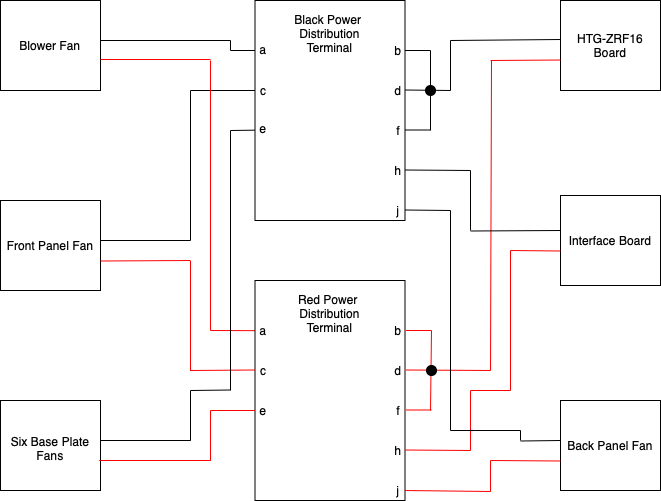
\includegraphics[width=1\linewidth]{figures/RFSoC_Power_Schematic_2.png}
\caption{RFSoC Digitizer Module Power Schematic Part 2. This half of the power schematic shows the connections of the two power distribution terminals, the fans, the HTG-ZRF16 board, and the Interface Board. The colors of the connections represent the color of wire used. The wire gauges are specified  in the power supply subsections.}
\label{fig:RFSoC_Power_Schematic_2}
\end{figure}
% ----------------------------------------------------------------

\subsection{The Power Entry Module}
\label{sec:6.6}
% ----------------------------------------------------------------

The power entry module (PN: 4304.4005) is connected to the power supply (PN: 13100-151) and the base plate. Refer to Figure \ref{fig:RFSoC_Power_Schematic_1} for the wiring schematic of the power entry module.

Th power supply connection to the power entry module was already described in the previous section. The base plate is connected to the power entry module via a green 12 awg wire crimped with a 6s eye terminal on one end and a female piggyback disconnect terminal (PN:
PBDD2-250) on the other. The 6s eye terminal is screwed into the base plate while the female piggyback disconnect terminal plugs into the power entry module. Note that this is the female piggyback disconnect terminal that has the the green ground wire from the power supply plugging into it. 


%----------------------------------------------------------------------------------------
%	Completed Module
%----------------------------------------------------------------------------------------
\section{Completed Module}
\label{sec:7}
% ----------------------------------------------------------------

Upon completion, an assembled RFSoC Digitizer Module is shown in the Figures \ref{fig:Enclosure_above}, \ref{fig:Front_completed}, \ref{fig:Back_complete}, and \ref{fig:Enclosure_in_Rack}. The biggest difference between the finished enclosure and the CAD design is the wiring, screws, lids, and cable clamp (front middle between the front panel and RFSoC board in Figure \ref{fig:Enclosure_above}) which were all left out in the CAD (Figures \ref{fig:CAD-Iso} and \ref{fig:CAD-top}). Note that the new heat sink and fan had not yet been installed on the HTG-ZRF16 board in Figure \ref{fig:Enclosure_above}. Furthermore, Figures  \ref{fig:Front_completed} and \ref{fig:Back_complete} is missing the HTG-ZRF16
board and so, in turn, is missing the feed throughs on the front and back panels.


\begin{figure}[H]
\centering
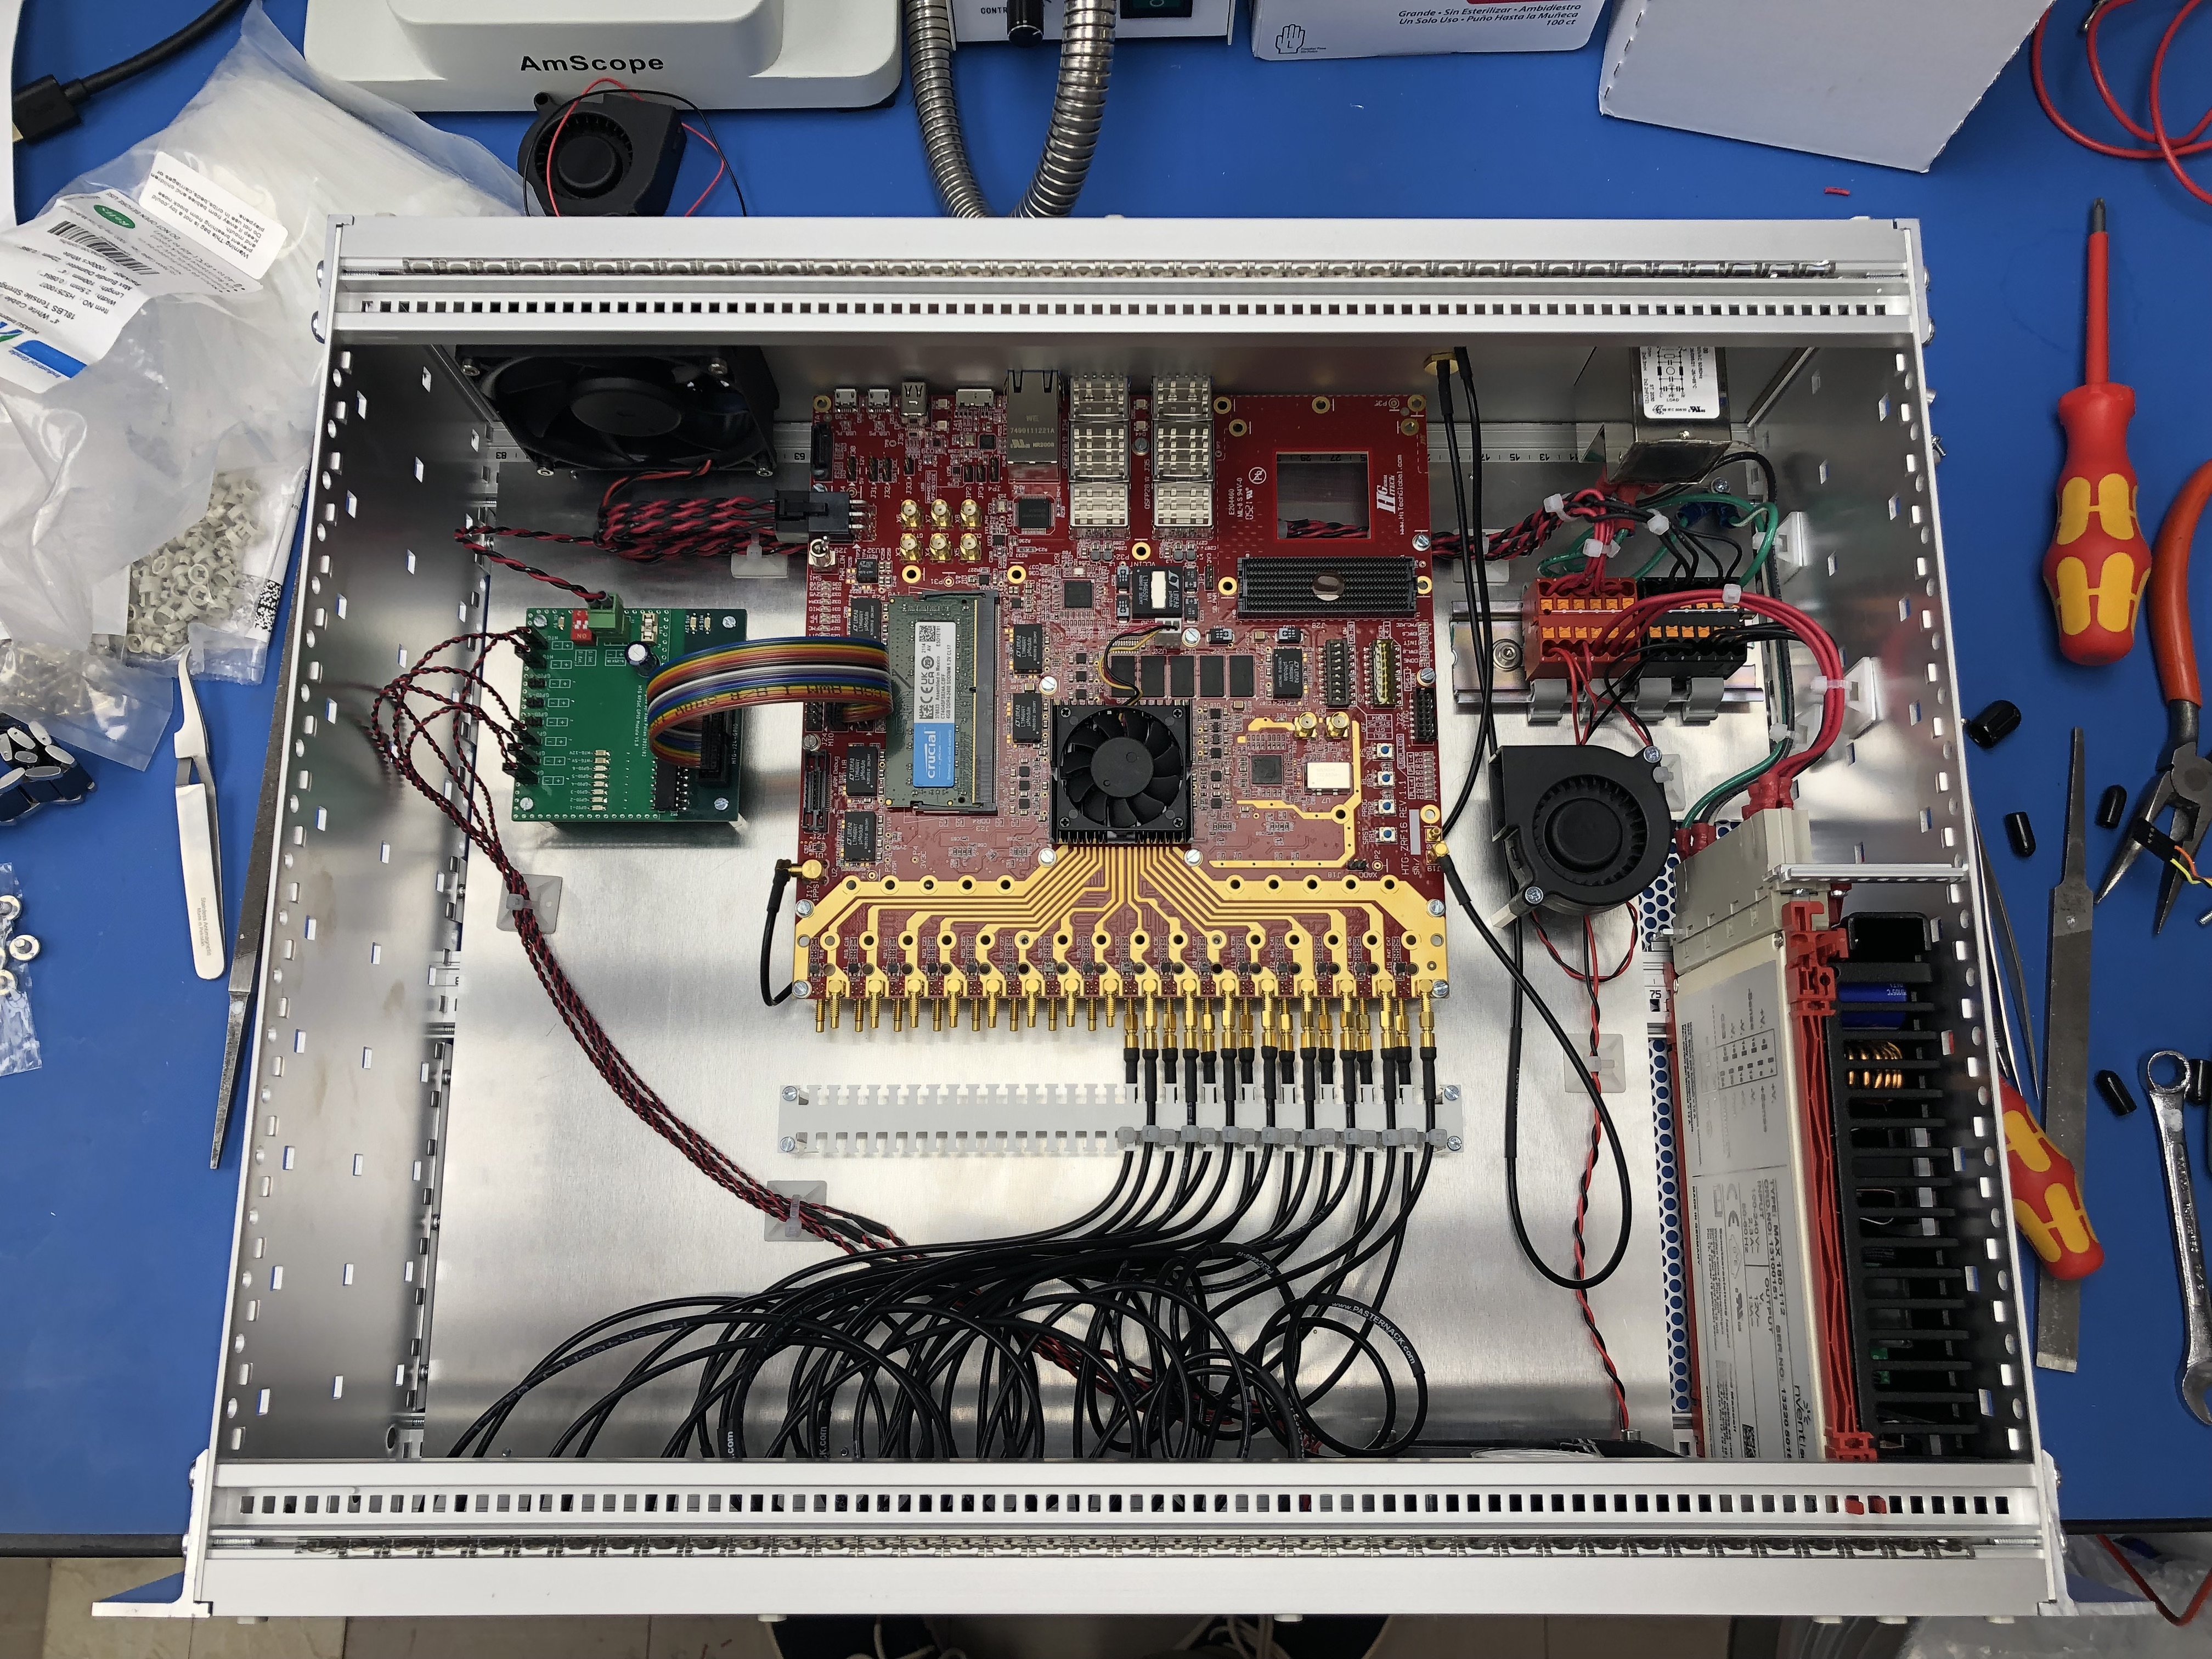
\includegraphics[width=1\linewidth]{figures/Finished_top_view.jpeg}
\caption{Completed RFSoC Digitizer Module}
\label{fig:Enclosure_above}
\end{figure}

\begin{figure}[H]
\centering
\includegraphics[width=.9\linewidth]{figures/Front_completed.jpeg}
\caption{Mostly Completed RFSoC Digitizer Module from the Front}
\label{fig:Front_completed}
\end{figure}

\begin{figure}[H]
\centering
\includegraphics[width=.9\linewidth]{figures/Back_complete.jpeg}
\caption{Mostly Completed RFSoC Digitizer Module from the Back}
\label{fig:Back_complete}
\end{figure}

\begin{figure}[H]
\centering
s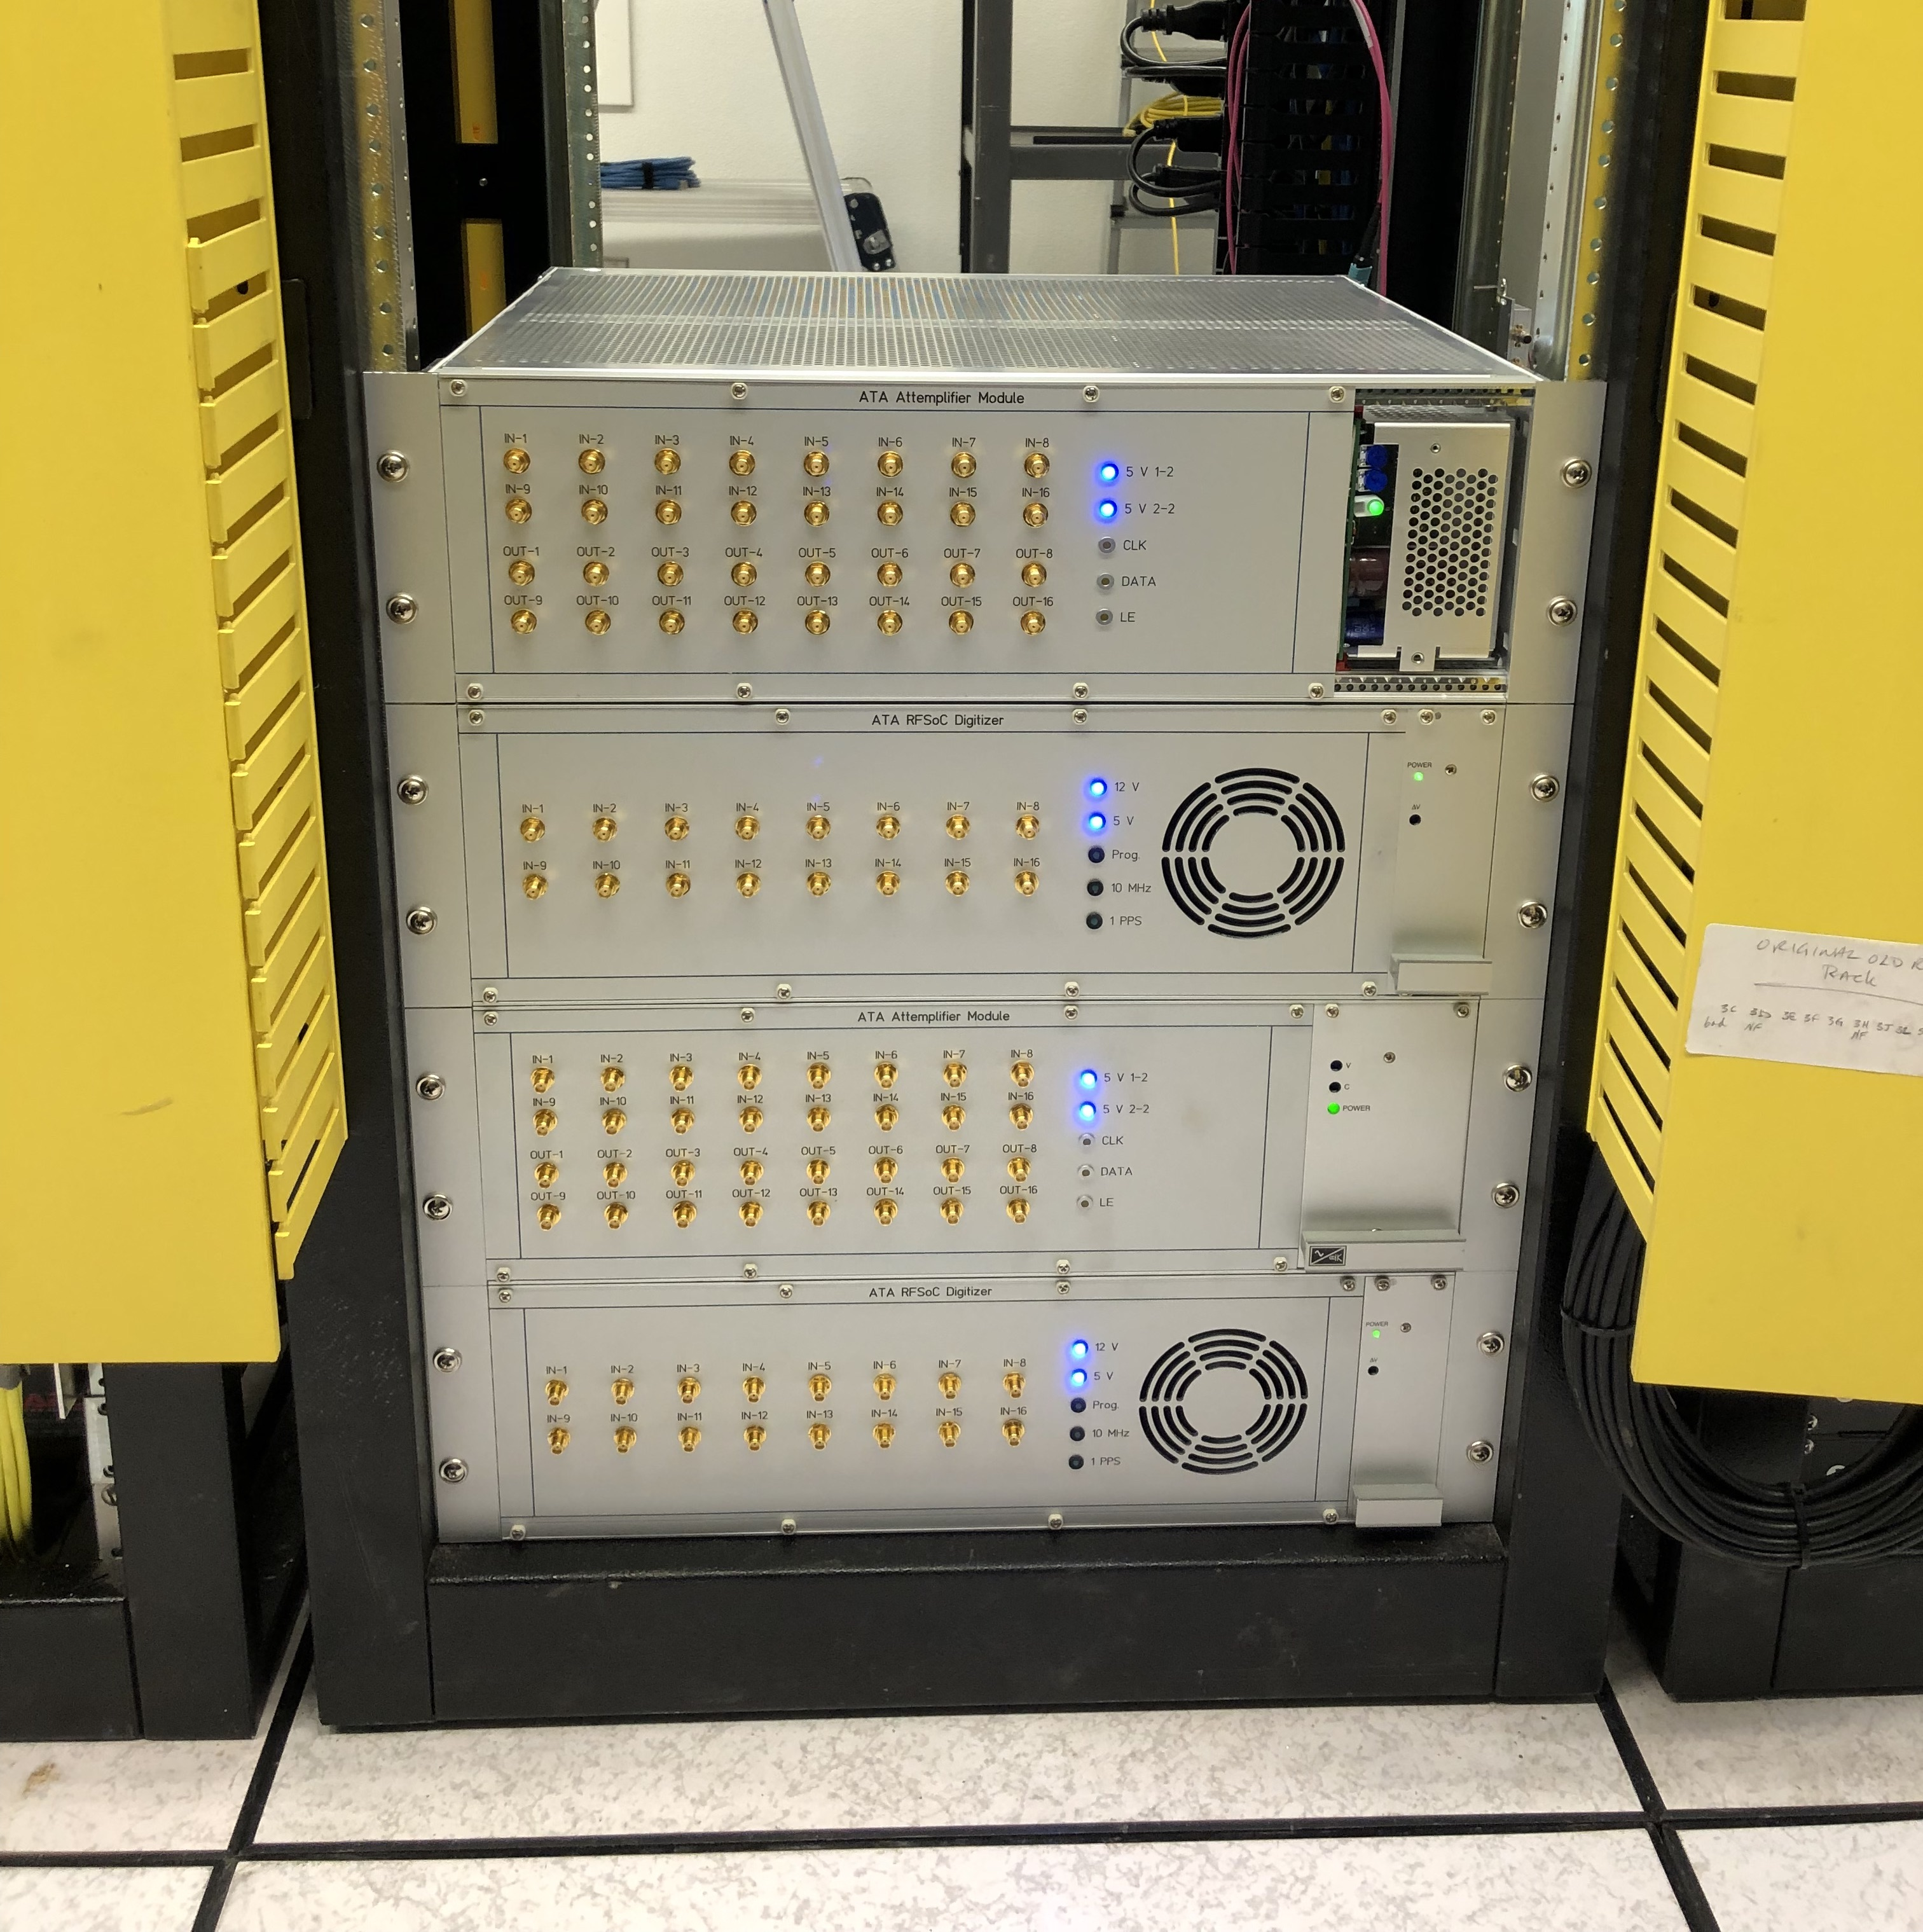
\includegraphics[width=.9\linewidth]{figures/Installed_in_Rack.jpeg}
\caption{Completed RFSoC Digitizer Module Installed in Signal Processing Room. Attemplifier Modules are also pictured. The RFSoC Digitizer Modules are the first and third modules from the bottom.}
\label{fig:Enclosure_in_Rack}
\end{figure}

\newpage


%----------------------------------------------------------------------------------------
%	Appendix A: RFSoC Enclosure Drawings
%----------------------------------------------------------------------------------------

\appendix
% ----------------------------------------------------------------


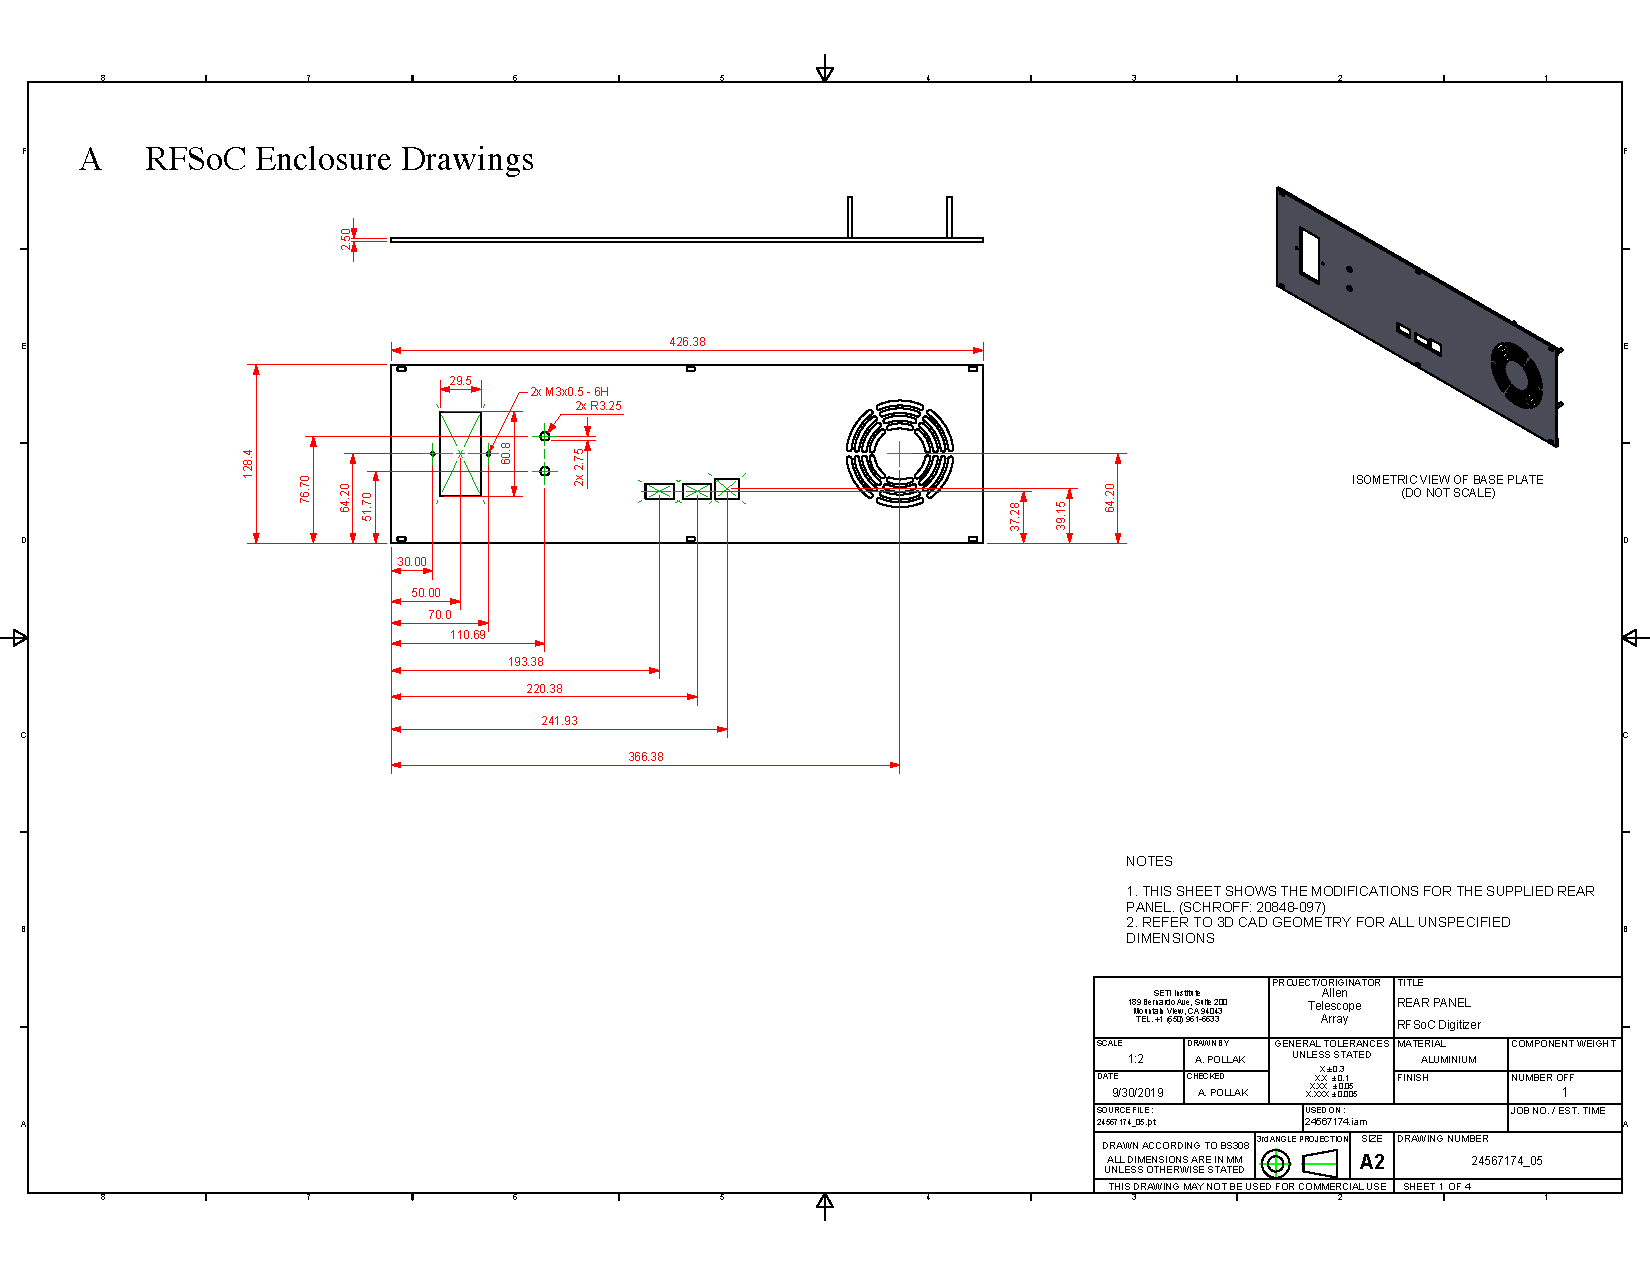
\includepdf[pages=-, landscape=true]{PDFs/24567174_05 (copy).pdf}
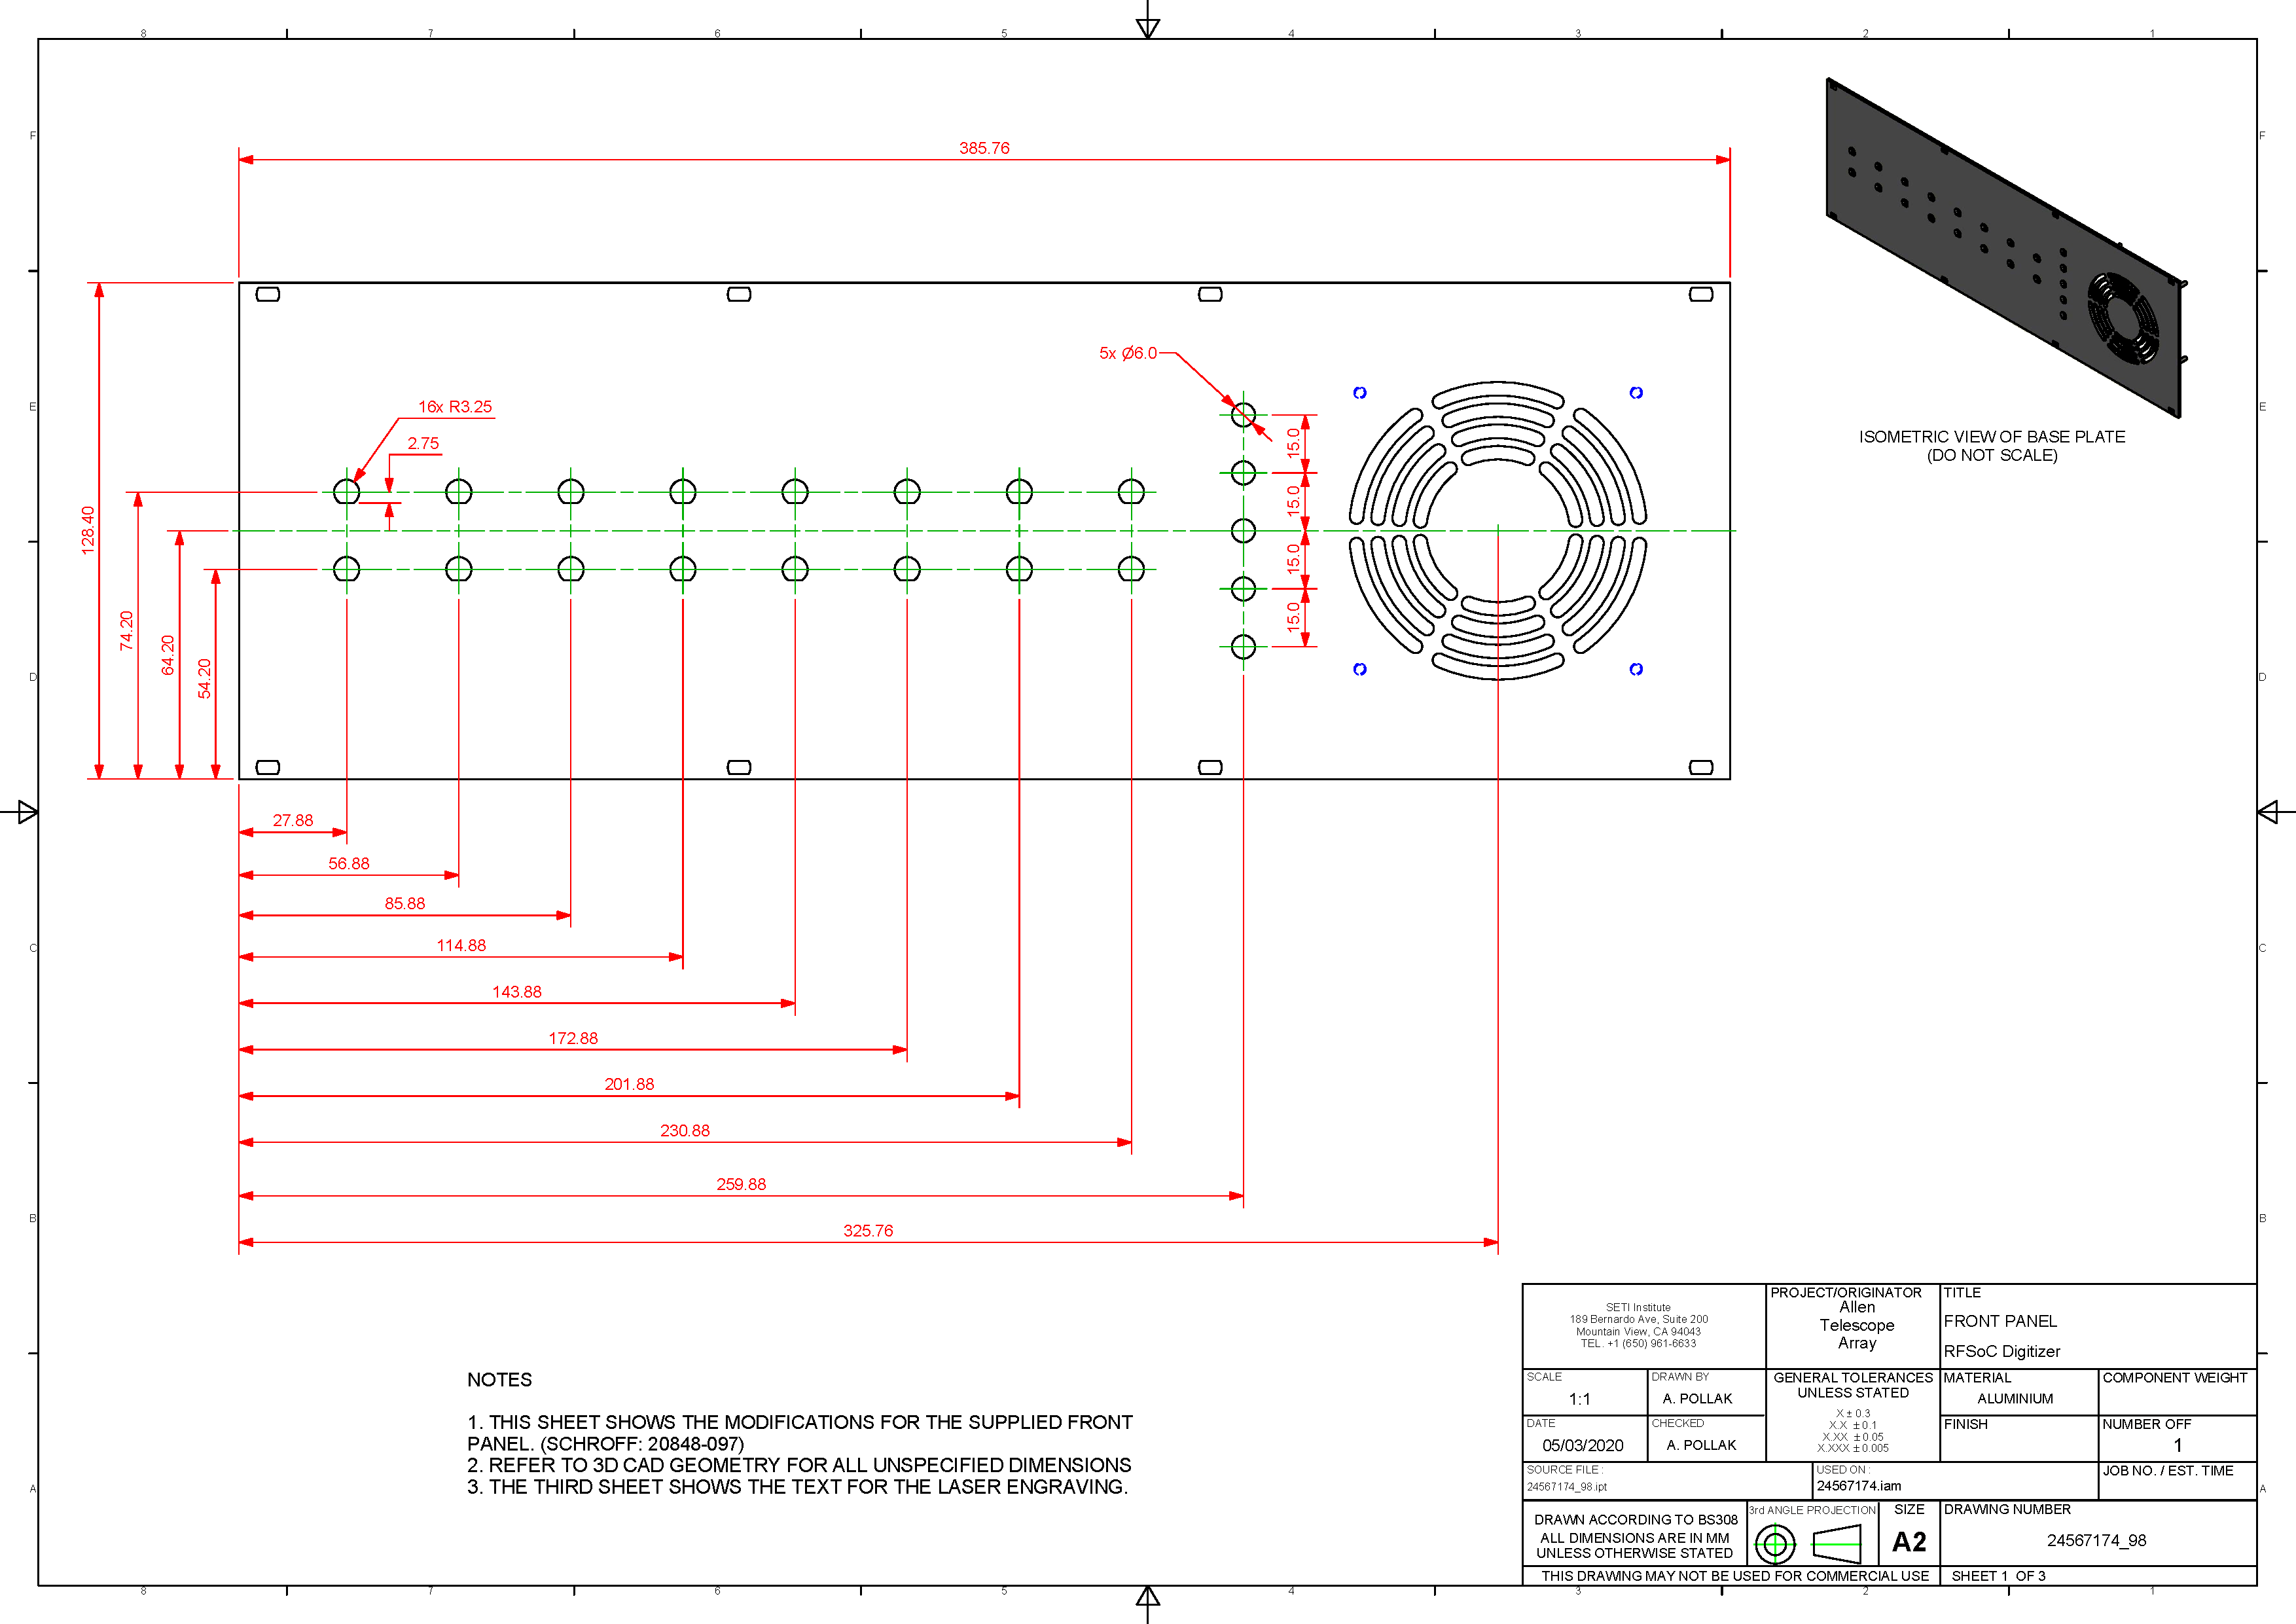
\includepdf[pages=-, landscape=true]{PDFs/24567174_98.pdf}
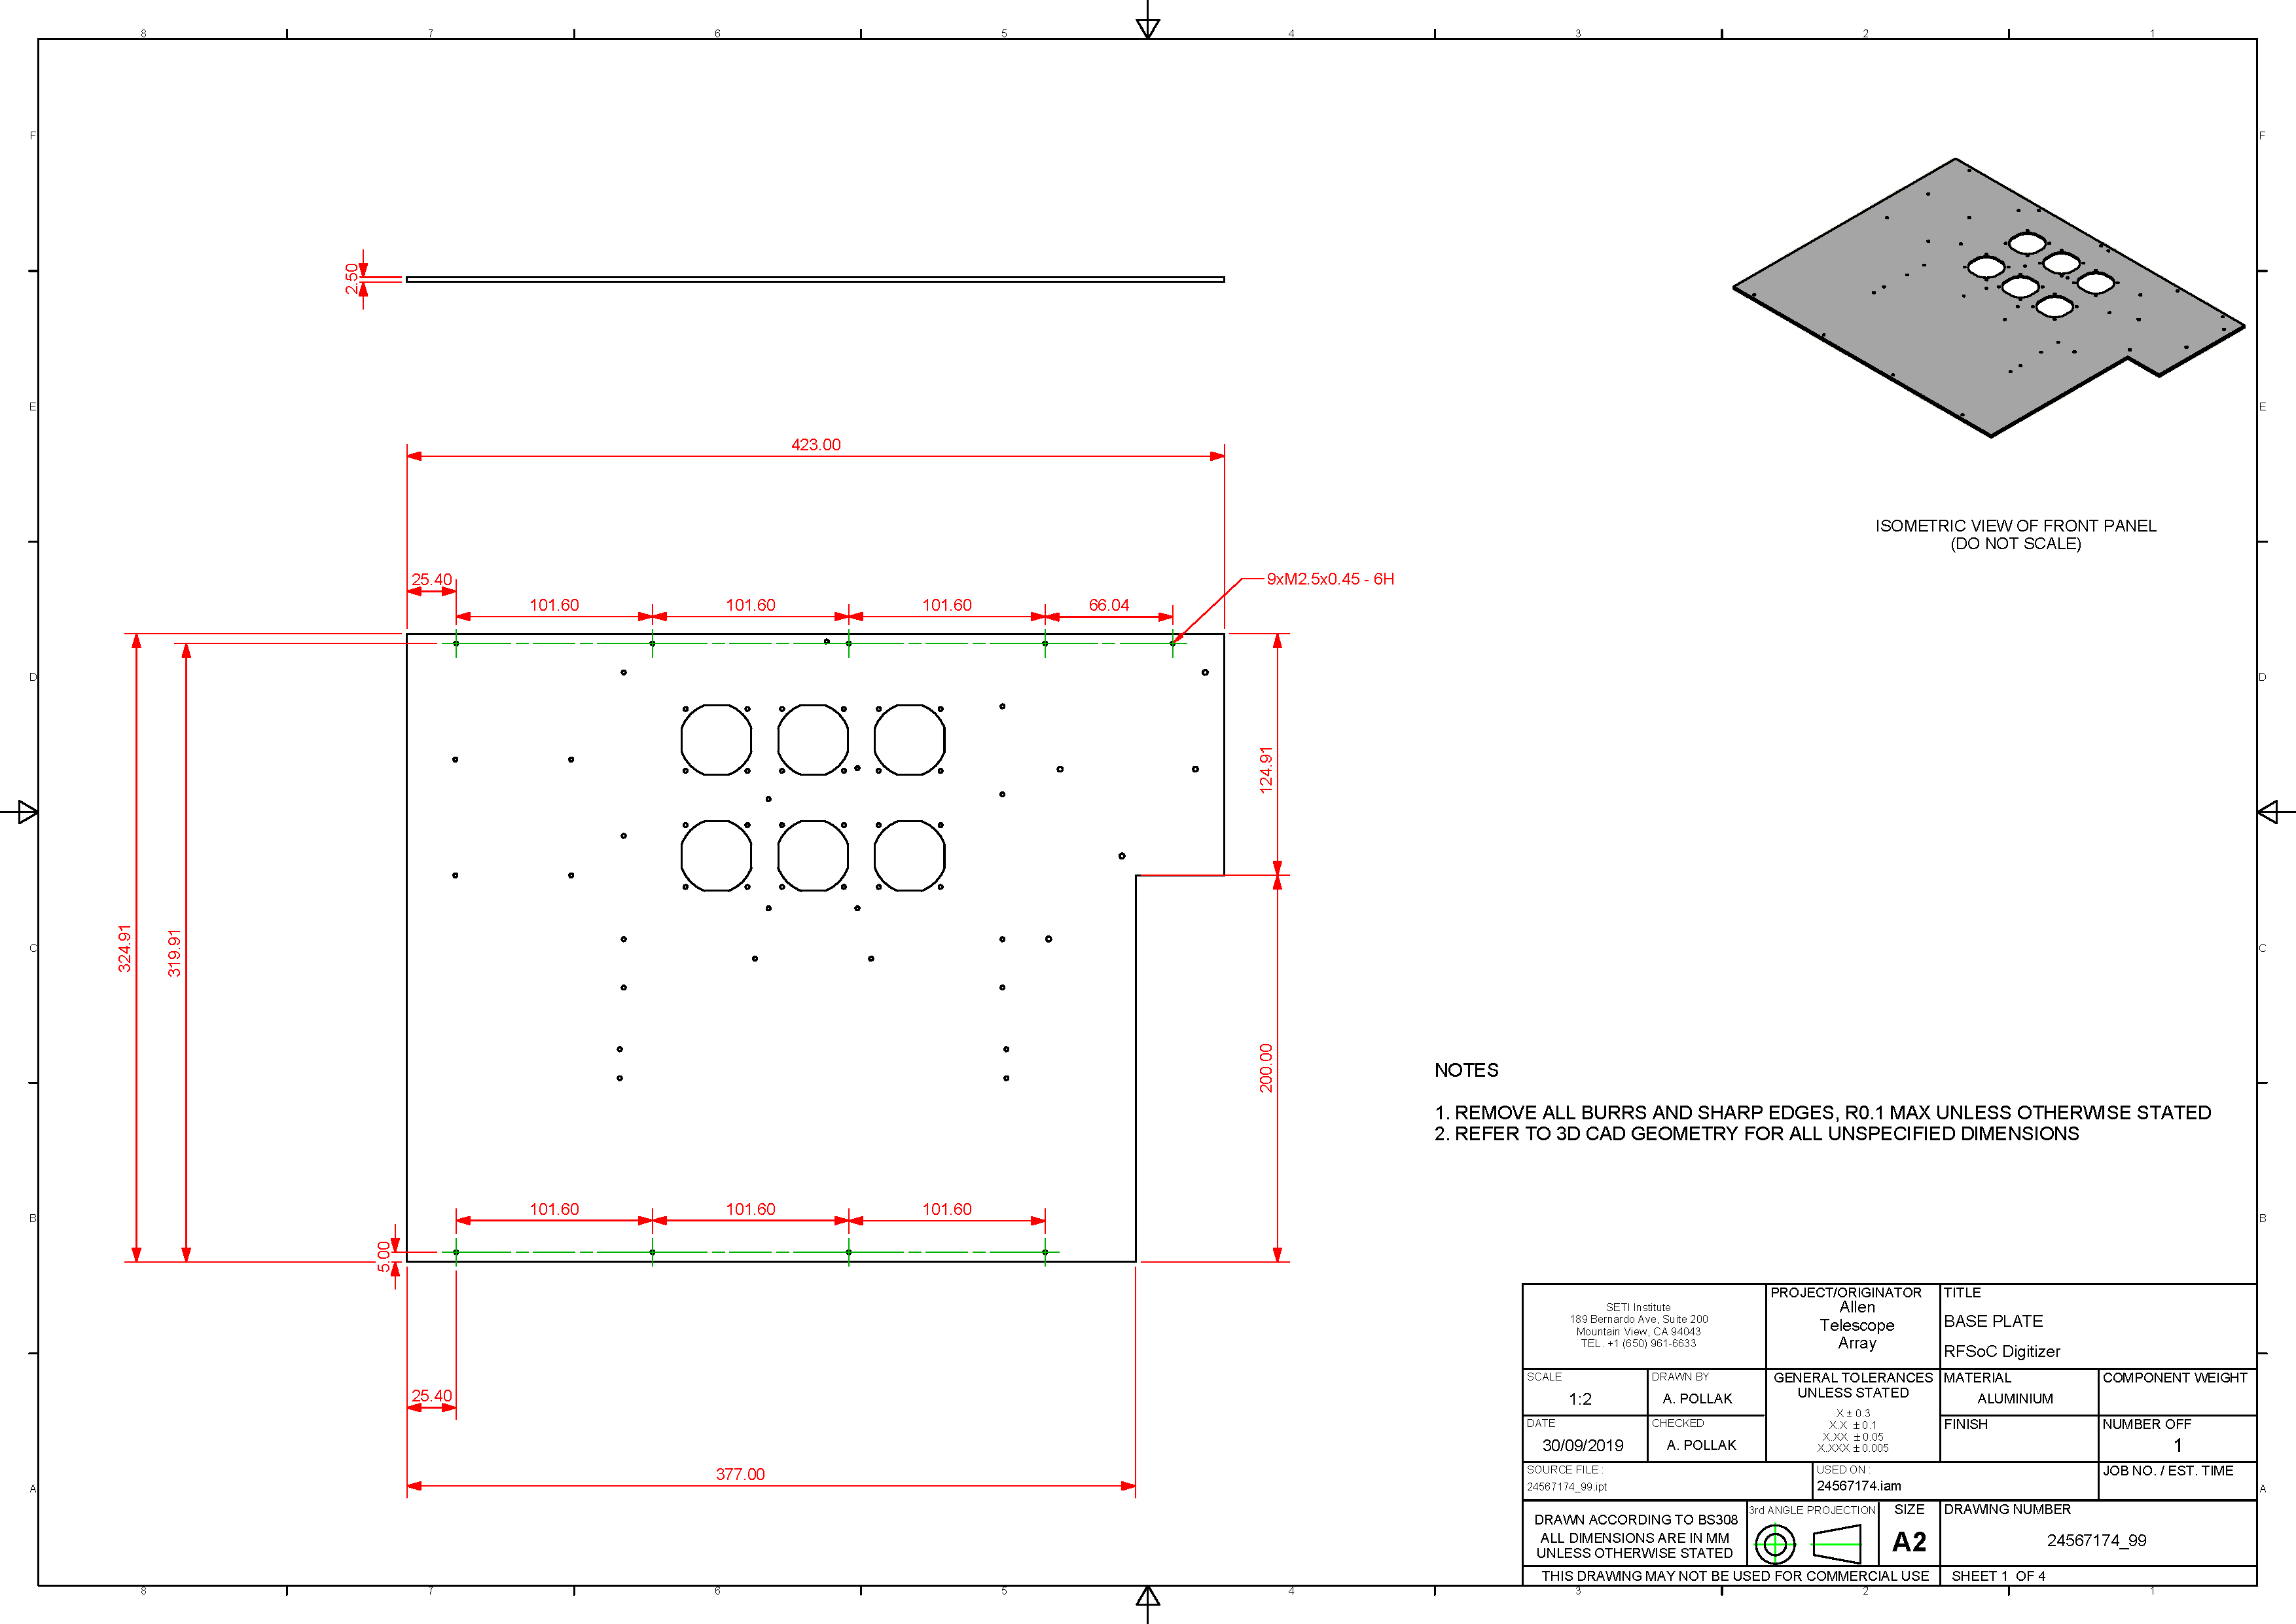
\includepdf[pages=-, landscape=true]{PDFs/24567174_99.pdf}
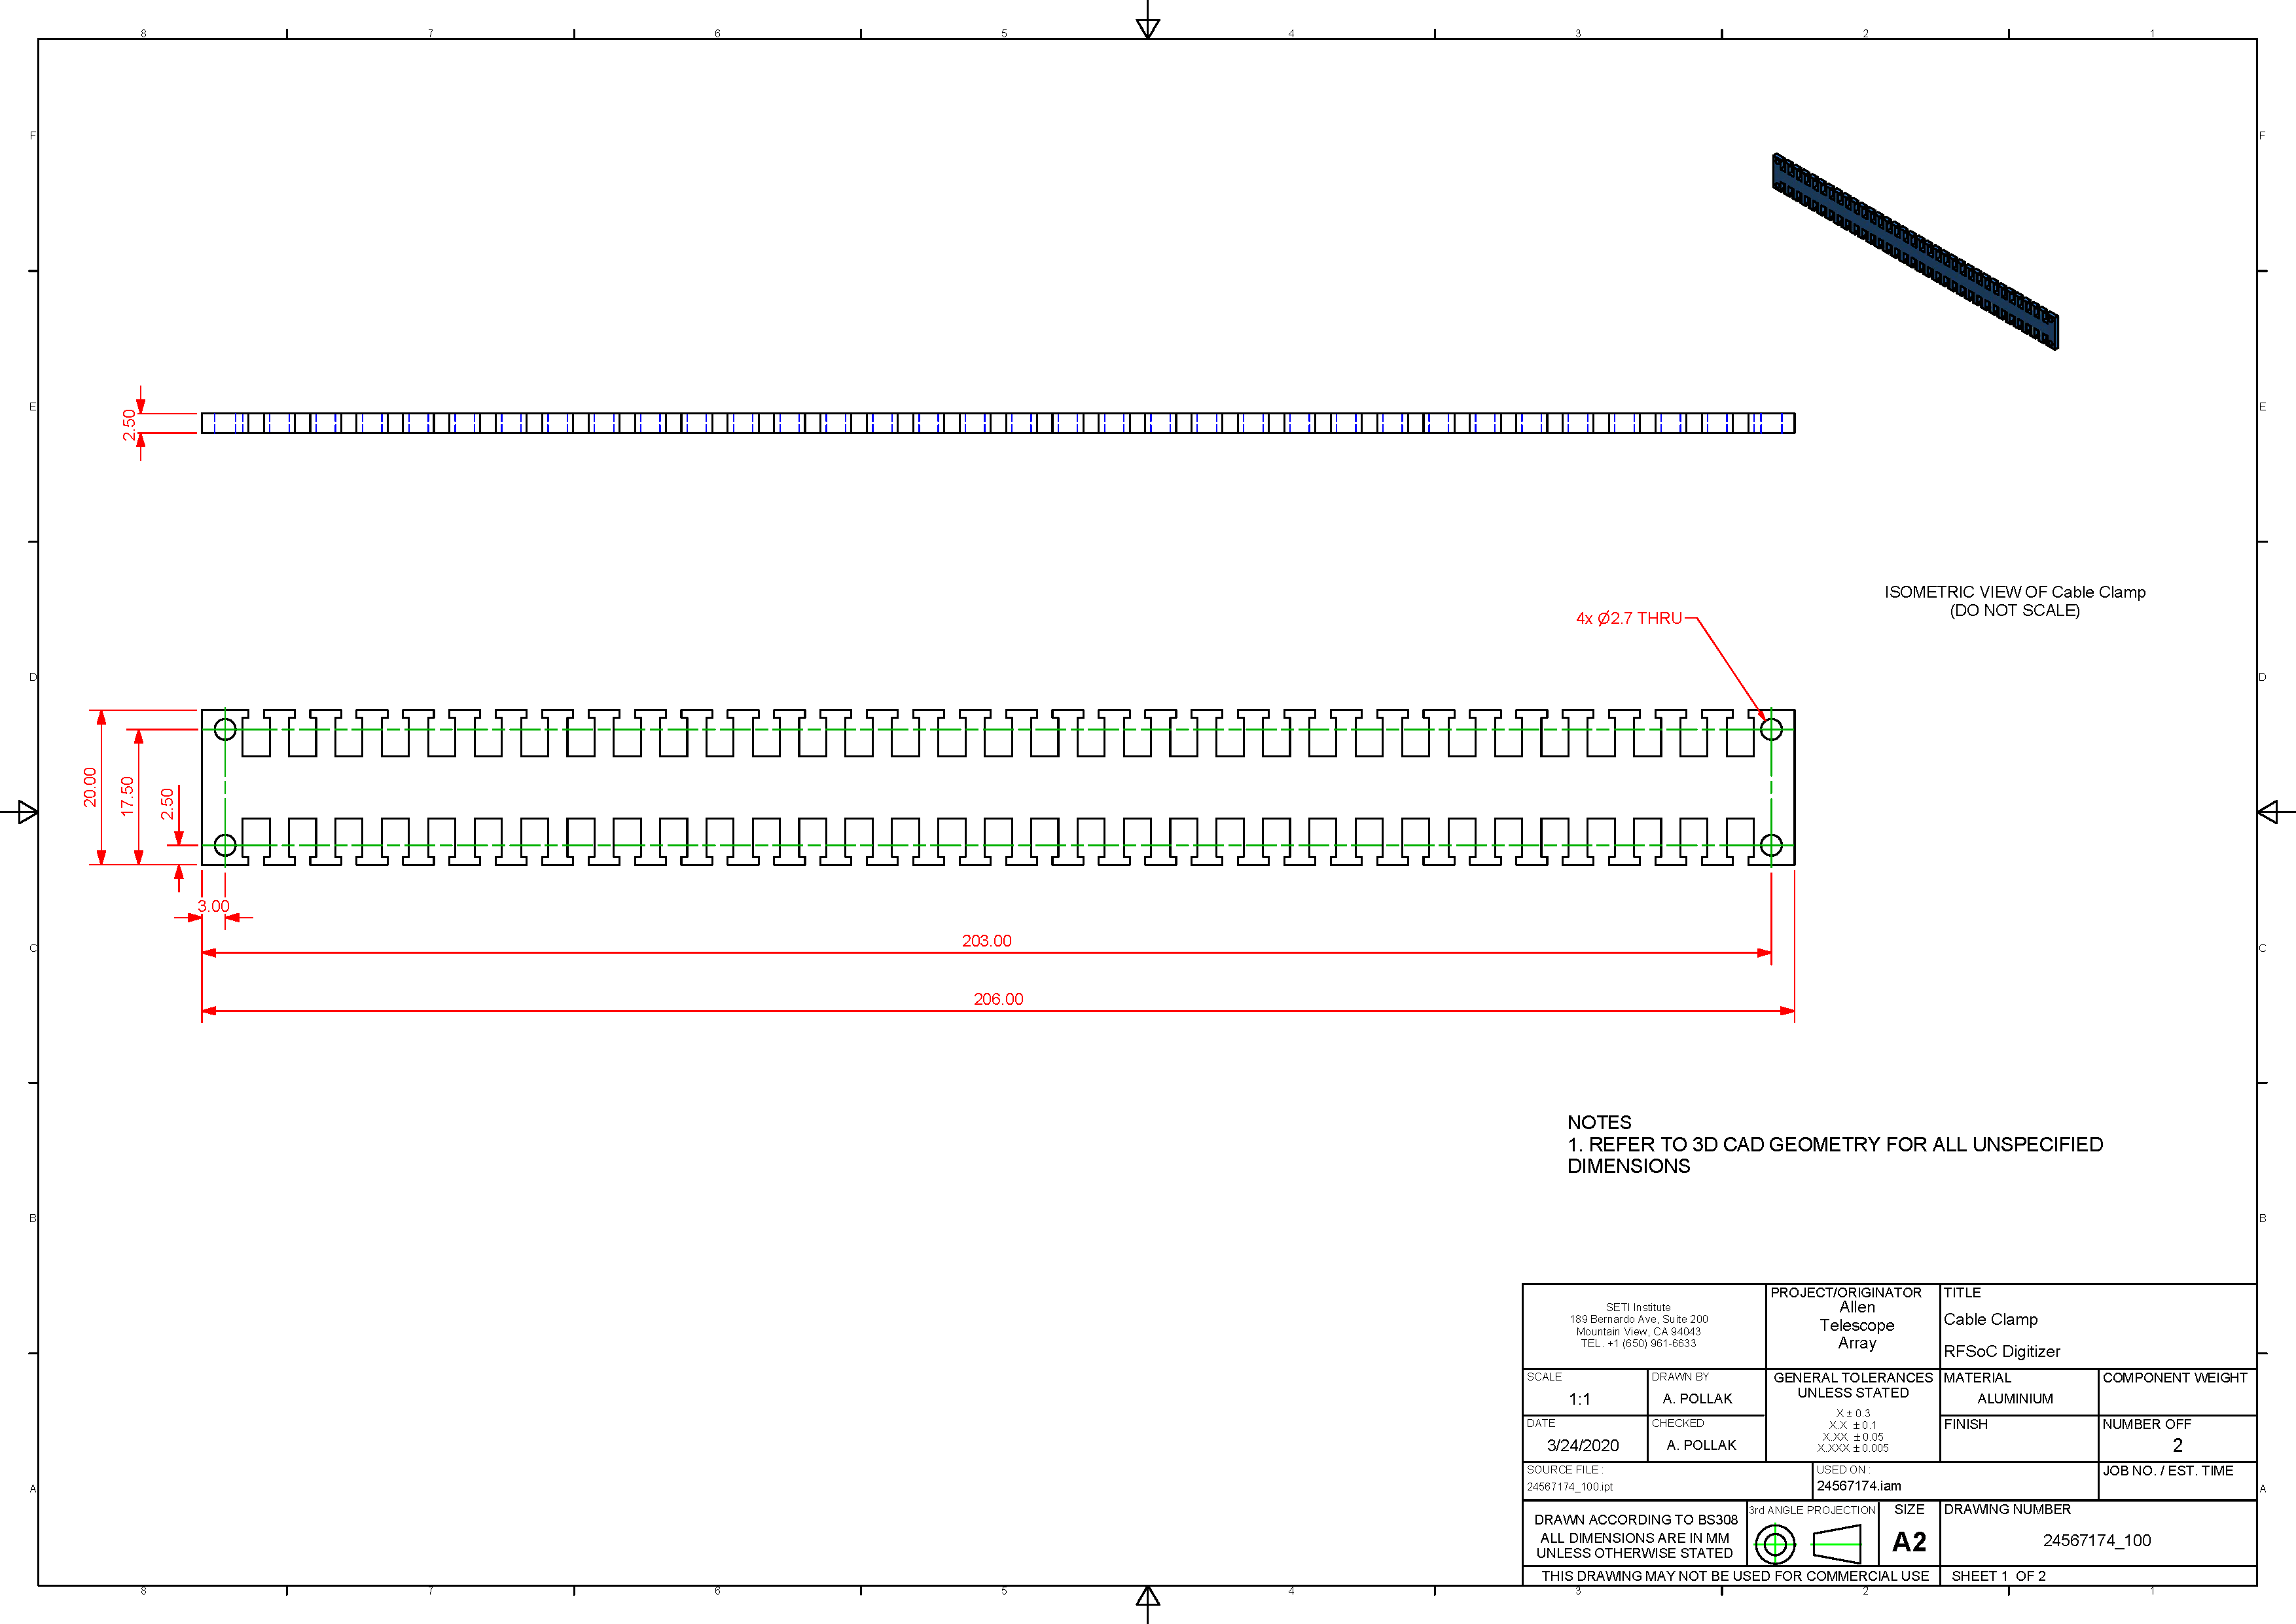
\includepdf[pages=-, landscape=true]{PDFs/24567174_100.pdf}

%----------------------------------------------------------------------------------------
%	Appendix B: RFSoC Digitizer Module Component List
%----------------------------------------------------------------------------------------
\begin{landscape}
\section*{B \hspace{.5cm} Component List of RFSoC Digitizer Module}

% ----------------------------------------------------------------

\begin{table}[H]
\centering
\resizebox{1.5\textwidth}{!}{%
\begin{tabular}{@{}lllllll@{}}
\toprule
Qty & Unit & Description & Manufacturer & PN Manufacturer & Distributor & PN Distributor\\
\midrule
1 & Each & EuropacPRO kit, heavy design, shielded, with front handles & Schroff & 
24567-174 & Distrelec & 110-74-433\\
1 & Each & 19" AC/DC switch-mode PSUs, maxpower 180 W, single 12V 13A & Schroff & 13100-151 & Distrelec & 110-89-774\\
1 & Each & Front Panel 13100 SLE 19" AC/DC Switch-Mode PSUs 128.4 mm, nVent Schroff & Schroff & 31006-677 & Distrelec & 110-90-375\\
1 & Each & Coding, PU 10 pack & Schroff & 20800-042  & Distrelec & 110-89-865\\
1 & Pack & Guide Rail Standard Type, Red, 160mm, Pack of 10 pieces & Schroff & 24568-361 & Distrelec & 302-25-177\\
1 & Each & Connector H 15 F, FASTON connection & Schroff & 69001-733 & Distrelec & 110-90-542\\
1 & Each & Front Panel & Front Panel Express, LLC & ATA-AP-24567174\_98.fpd\\
1 & Each & Rear Panel & Front Panel Express, LLC  & ATA-AP-24567174\_05.fpd\\
1 & Each & Baseplate & Front Panel Express, LLC & ATA-AP-24567174\_99.fpd\\
1 & Each & Cable Clamp & Front Panel Express, LLC  & ATA-AP-24567174\_100.fpd\\
1 & Each & DC Fans DC Fan, High Airflow Series, 80x80 & Sunon & PF80251V1-1000U-A99  & Mouser & 369-PF80251V11UA99\\
6 & Each & Axial Fan, IP20, 12 V, DC, 40 mm, 10 mm & EBM-PAPST & 412FM & Mouser & 5912-412FM\\
1 & Each & Fan Blower, GB Series, Compact, 12 V, DC & SUNON & GB1205PKV1-8AY.GN & Mouser & 369-GB1205PKV18AYGN\\
1 & Pack & Screw, SLT, CSK, Steel, BZP, M3X16 & TR Fastenings & M316 KSSTMCZ100- & Newark & 53M8739\\ 
1 & Pack & Enclosure Accessory, Grey, Plastic Sleeve & Schroff & 21100-464 & Newark & 74M6491\\
1 & Pack & 21101-101 -  COLLAR SCREW, PK100 & Schroff & 21101-101 & Newark & 74M6493\\
1 & Each & 4304.4005 -  INLET FILTER, IEC, C14, FKH, 10A & Schurter & 43044005 & Newark & 83T7492\\
6 & Each & Standoffs \& Spacers M3 x 25mm HEX & Harwin  & R30-3002502 & Mouser & 855-R30-3002502\\
25 & Each & Standoffs, Hex Male-Female, 20MM, M2.5 & RAF & M2115-2545-AL & Mouser & 761-M2115-2545-AL\\
1 & Each & DIN rail perforated & Phoenix Contact & 801733 & Mouser & 651-0801733\\
1 & Each & DIN Rail Terminal Blocks PTFIX 12X2,5-NS35ARD 2.5mm2  & Phoenix Contact & 3273158 & Mouser & 651-3273158\\
1 & Each & DIN Rail Terminal Blocks PTFIX 12X2,5-NS35ABK 2.5mm2 & Phoenix Contact & 3273168 & Mouser & 651-3273168\\
1 & Each & Headers \& Wire Housings 6CKT RECPT HSG & Molex & 45559-0002 & Mouser & 538-45559-0002\\
100 & Each & Headers \& Wire Housings MF PLUS HCS CRIMP TE RM. FEM 18-20 GA TIN & Molex & 45750-1112 & Mouser & 538-45750-1112\\
1 & Each & Extraction, Removal \& Insertion Tools EXTRACTION TOOL & Molex & 11-03-0044 & Mouser & 538-11-03-0044\\
1 & Each & Crimpers / Crimping Tools MINI-FIT 18-24AWG HAND TOOL & Molex & 63819-0901 & Mouser & 538-63819-0901\\
16 & Each & SMA Female Bulkhead to SSMC Plug Cable 18 Inch Length Using PE-SR405FLJ Coax & Pasternack & PE3C4448-18 & Pasternack & PE3C4448-18\\
1 & Each & SMA Female Bulkhead to MCX Plug Right Angle Semi-Flexible Precision Cable 18 Inch Length Using PE-SR405FLJ Coax, LF Solder, RoHS & Pasternack & PE39435-18 & Pasternack & PE39435-18\\
1 & Each & SMA Female Bulkhead to SSMC Plug Right Angle Cable 18 Inch Length Using PE-SR405FLJ Coax & Pasternack & PE3C4486-18 & Pasternack & PE3C4486-18\\
5 & Each & LED Panel Mount Indicator, Blue, 3.8 VDC, 6 mm, 20 mA & APEM & Q6F7BXXB02E & Mouser & 642-Q6F7BXXB02E\\
2 & Pack & SCREW,SECURITY FIXING, M2,5X5, PK100 & VERO & 173-202579H & Newark & 25M0782\\
1 & Pack & Machine Screw, M3, 25 mm & & & Newark & 27AC4115\\
2 & Each & Fuse, Cartridge, Slow Blow, 2 A, 250 V & Littlefuse & 0239002.HXP & Newark & 26K8412\\



\bottomrule            
\end{tabular}}
\label{tab:Interface_components}
\end{table}

\newpage

%----------------------------------------------------------------------------------------
%	Appendix C: Interface Board and HTG-ZRF16 board Component List
%----------------------------------------------------------------------------------------

\section*{C \hspace{.5cm} Interface Board and HTG-ZRF16 board Component List}

% ----------------------------------------------------------------

\begin{table}[H]
\centering
\resizebox{1.5\textwidth}{!}{%
\begin{tabular}{@{}lllllll@{}}
\toprule
Qty & Unit & Description & Manufacturer & PN Manufacturer & Distributor & PN Distributor\\
\midrule

1 & Each & ATA\_HTG\_ZRF16\_GPIO\_Board\_AP\_V1.0 & AP\\
1 & Each & PCB V1.0 & AP & ATA\_HTG\_ZRF16\_GPIO\_Board\_AP\_V1.0.zip\\
1 & Each & Littelfuse 1A T Non-Resettable Surface Mount Fuse, 125 V & Littlefuse & 0154001.DRT & Mouser & 576-0154001.DRT\\
1 & Each & Fuse, Surface Mount, 1.5 A, NANO 452 Series, 125 VAC, 32 VDC, Time Delay, SMD & Littlefuse & 045201.5MRL & Mouser & 576-045201.5MRL\\
1 & Each & Surface Mount Tantalum Capacitor, $100 \mu F$, 25 V, 2917 [7343 Metric], T491 Series, $\pm 10\%, -55 \degree C$ & Kemet & T491X107K025AT & Mouser & 80-T491X107K025AT\\
1 & Each & Electrolytic Capacitor, 220 $\mu F$, 35 V, M Series, $\pm 20\%$, Radial Leaded, 8 mm & PANASONIC & ECA-1VM221 & Mouser & 667-ECA-1VM221\\
1 & Each & KEMET C0805C224K1RACTU 220nF Multilayer Ceramic Capacitor MLCC 100V dc $\pm 10\%$ Tolerance SMD & Kemet & C0805C224K1RACTU & Mouser & 80-C0805C224K1R\\
1 & Each & KEMET C0805C104K5RACTU 100nF Multilayer Ceramic Capacitor MLCC 50V dc $\pm 10\%$ Tolerance SMD & Kemet & C0805C104K5RACTU & Mouser & 80-C0805C104K5R\\
1 & Each &  LINEAR VOLT REG, 5V, 1.5A, TO-263-3 & Texas Instruments & LM340SX-5.0/NOPB & Mouser & 926-LM340SX-5.0/NOPB\\
5 & Each & LED, QuasarBrite, Green, SMD, 1206, 20 mA, 2.2 V, 565 nm & LUMEX & SML-LX1206GW-TR  & Mouser & 696-SML-LX1206GW\\
6 & Each & LED, QuasarBrite, Yellow, SMD, 1206, 20 mA, 2 V, 590 nm & LUMEX & SML-LX1206SYC-TR & Mouser & 696-SML-LX1206SYC\\
1 & Each & Thin Film Resistors - SMD 0805 523ohm & Panasonic & ERA-6AEB5230V & Mouser & 667-ERA-6AEB5230V\\
18 & Each & Thin Film Resistors - SMD 0805 150ohms & Panasonic & ERA-6AEB151V & Mouser & 667-ERA-6AEB151V\\
1 & Each & Thin Film Resistors - SMD 0805 374ohm  & Panasonic & ERA-6AEB3740V & Mouser & 667-ERA-6AEB3740V\\
1 & Each & Thin Film Resistors - SMD 0805 1.07Kohm  & Panasonic & ERA-6AEB1071V & Mouser & 667-ERA-6AEB1071V\\
6(12) & Each & Thin Film Resistors - SMD 0805 200ohm & Panasonic & ERA-6AEB201V & Mouser & 667-ERA-6AEB201V\\
8 & Each & Thin Film Resistors - SMD 0805 4.7Kohms & Panasonic & ERA6AEB472V & Mouser & 667-ERA-6AEB472V\\
2 & Each & Optocoupler, Transistor Output, 4 Channel, DIP, 16 Pins, 60 mA, 5.3 kV, 100\% & VISHAY & ILQ2 & Mouser & 782-ILQ2\\
16 & Each & Buffers \& Line Drivers Single Schmitt-Trigger Buffer 5-SC70 -40 to 85 & Texas Instruments & SN74LVC1G17DCK3 & Mouser & 595-SN74LVC1G17DCK3\\
1 & Each & DIP Switches / SIP Switches SLIDE ACT 2 POS & Diptronics & NDS-02V & Mouser & 113-NDS-02V\\
1 & Each &  COMBICON MCV, 3.81mm Pitch, 2 Way, 1 Row, Straight PCB Terminal Block Header & Phoenix Contact & 1803426 & Mouser & 651-1803426\\
1 & Each & 2 way cable mount screw terminal, 3.81mm & Phoenix Contact & 1803578 & Mouser & 651-1803578\\
1 & Each & Headers \& Wire Housings 2.54mm CGrid Hdr Shr d /Slt .76AuLF 16Ckt & Molex & 70246-1602 & Mouser & 538-70246-1602\\
1 & Each & Headers \& Wire Housings 3CKT BRKWY HDR & Molex & 42375-1856 & Mouser & 538-42375-1856\\
8 & Each & Headers \& Wire Housings 2CKT BRKWY HDR & Molex & 42375-2486 & Mouser & 538-42375-2486\\
1 & Each & Ribbon Cables / IDC Cables 16Ckt & Samtec & IDSD-08-D-06.00 & Mouser & 200-IDSD08D0600\\
1 & Each & Headers \& Wire Housings 3 PIN SIL HOUSING & Harwin & M20-1060300 & Mouser & 855-M20-1060300\\
8 & Each & Headers \& Wire Housings 2 PIN SIL HOUSING & Harwin & M20-1060200 & Mouser & 855-M20-1060200\\
1 & Each & Headers \& Wire Housings F/M CRIMP TERM GOLD/TIN & Harwin & M20-1180042 & Mouser & 855-M20-1180042\\
1 & Each & Crimpers / Crimping Tools 2.54mm HAND CRIMP TOOL & Harwin & Z20-320 & Mouser & 855-Z20-320\\
1 & Each & Fan Tubeaxial 12VDC Square - 45mm L x 45mm H Ball 11.8 CFM (0.330m³/min) 2 Wire Leads & Delta Electronics & AFB04512HA & Digi-Key & 603-2157-ND\\
1 & Each & Heat Sink 45mm X 45mm X 24.5mm & Advanced Thermal Solutions & ATS-55450W-C1-R0 & Digi-Key & ATS1330-ND\\
2 & Each & Hex Standoff M2.5X0.45 Alum 20mm & RAF & M2115-2545-AL & Digi-Key & 1772-2060-ND\\
2 & Each & Mach Screw Pan Slotted M2.5X0.45 & Keystone Electronics & 29306 & Digi-Key & 36-29306-ND\\

\bottomrule            
\end{tabular}}
\label{tab:Attemp_components}
\end{table}

\newpage

%----------------------------------------------------------------------------------------
%	Appendix D: Interface Board Schematics
%----------------------------------------------------------------------------------------

\section*{D \hspace{.5cm} Interface Board Schematics}

% ----------------------------------------------------------------

%
\begin{figure}[H]
\centering
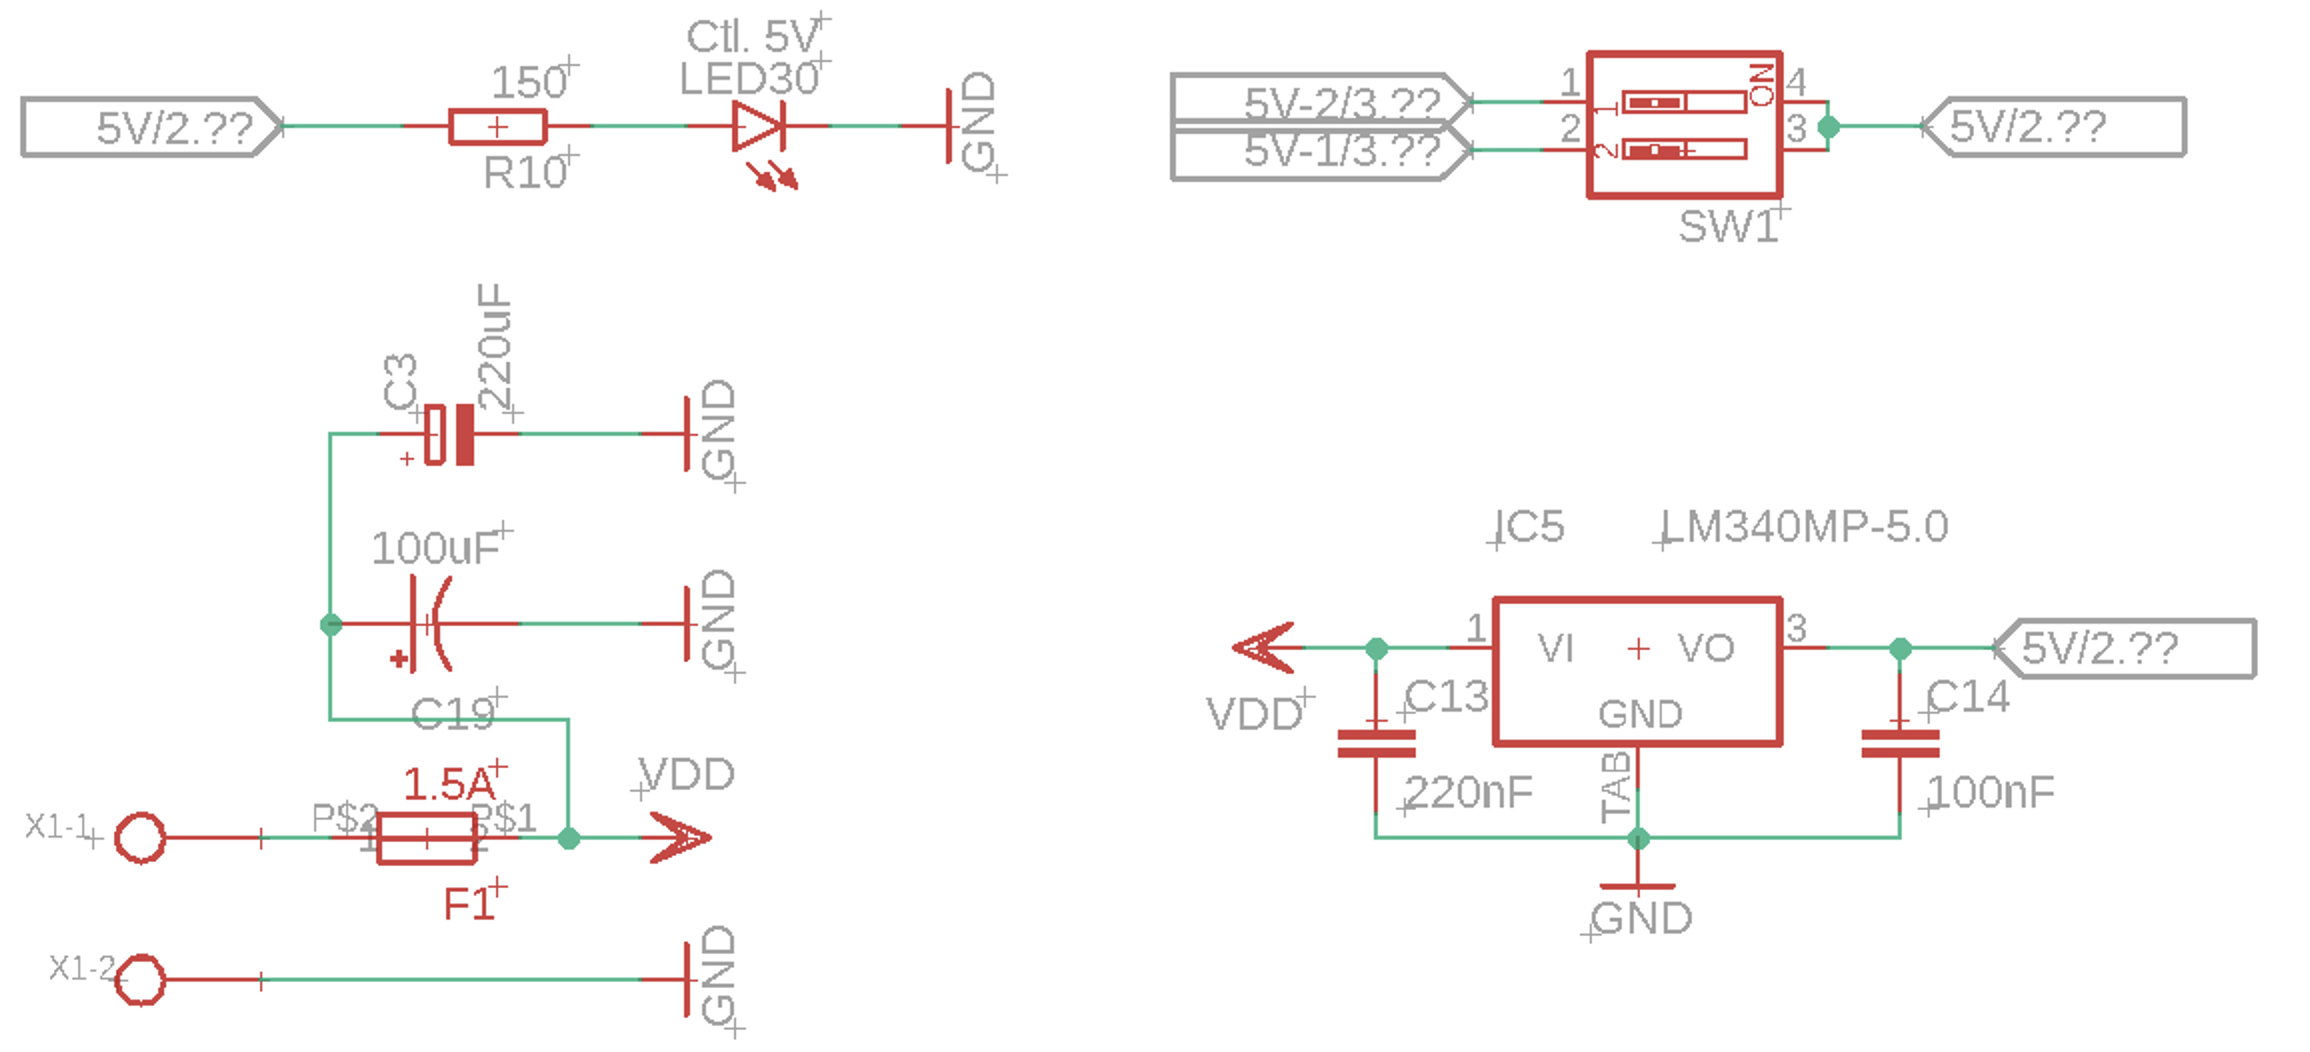
\includegraphics[width=1\linewidth]{figures/Interface_board_schematic_1.png}
\caption{Interface Board Schematic Part 1}
\label{fig:interface_sch1}
\end{figure}
%

\end{landscape}

%
\begin{figure}[H]
\centering
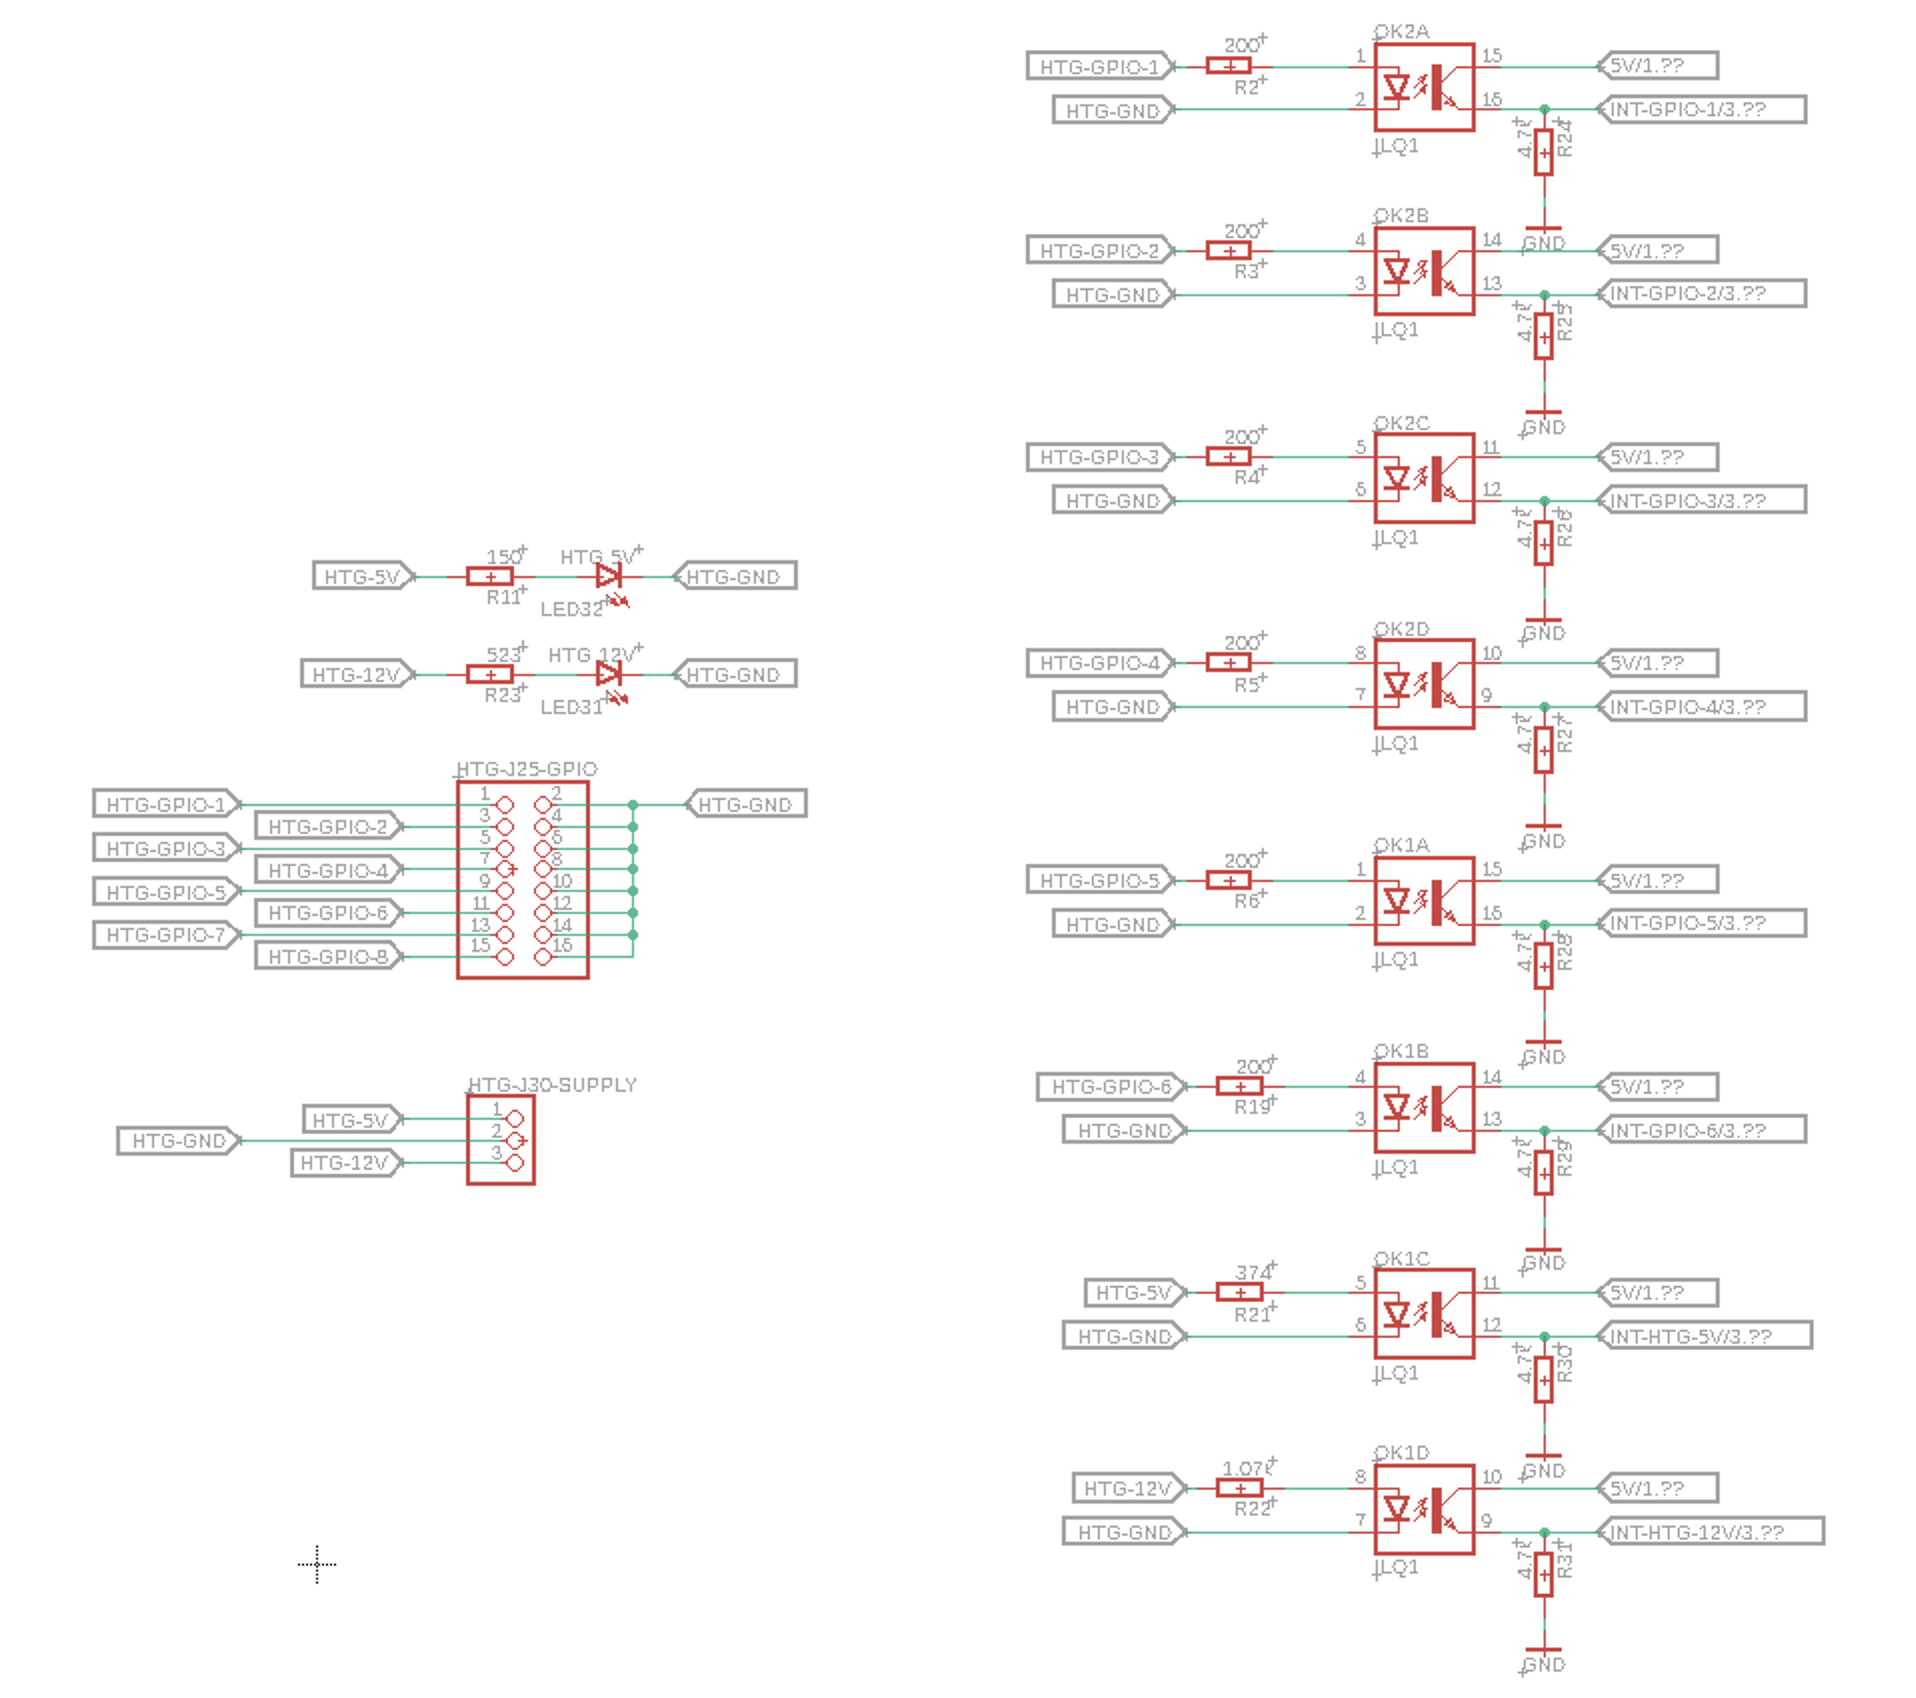
\includegraphics[width=1.1\linewidth]{figures/Interface_board_schematic_2.png}
\caption{Interface Board Schematic Part 2}
\label{fig:interface_sch2}
\end{figure}
%

%
\begin{figure}[H]
\centering
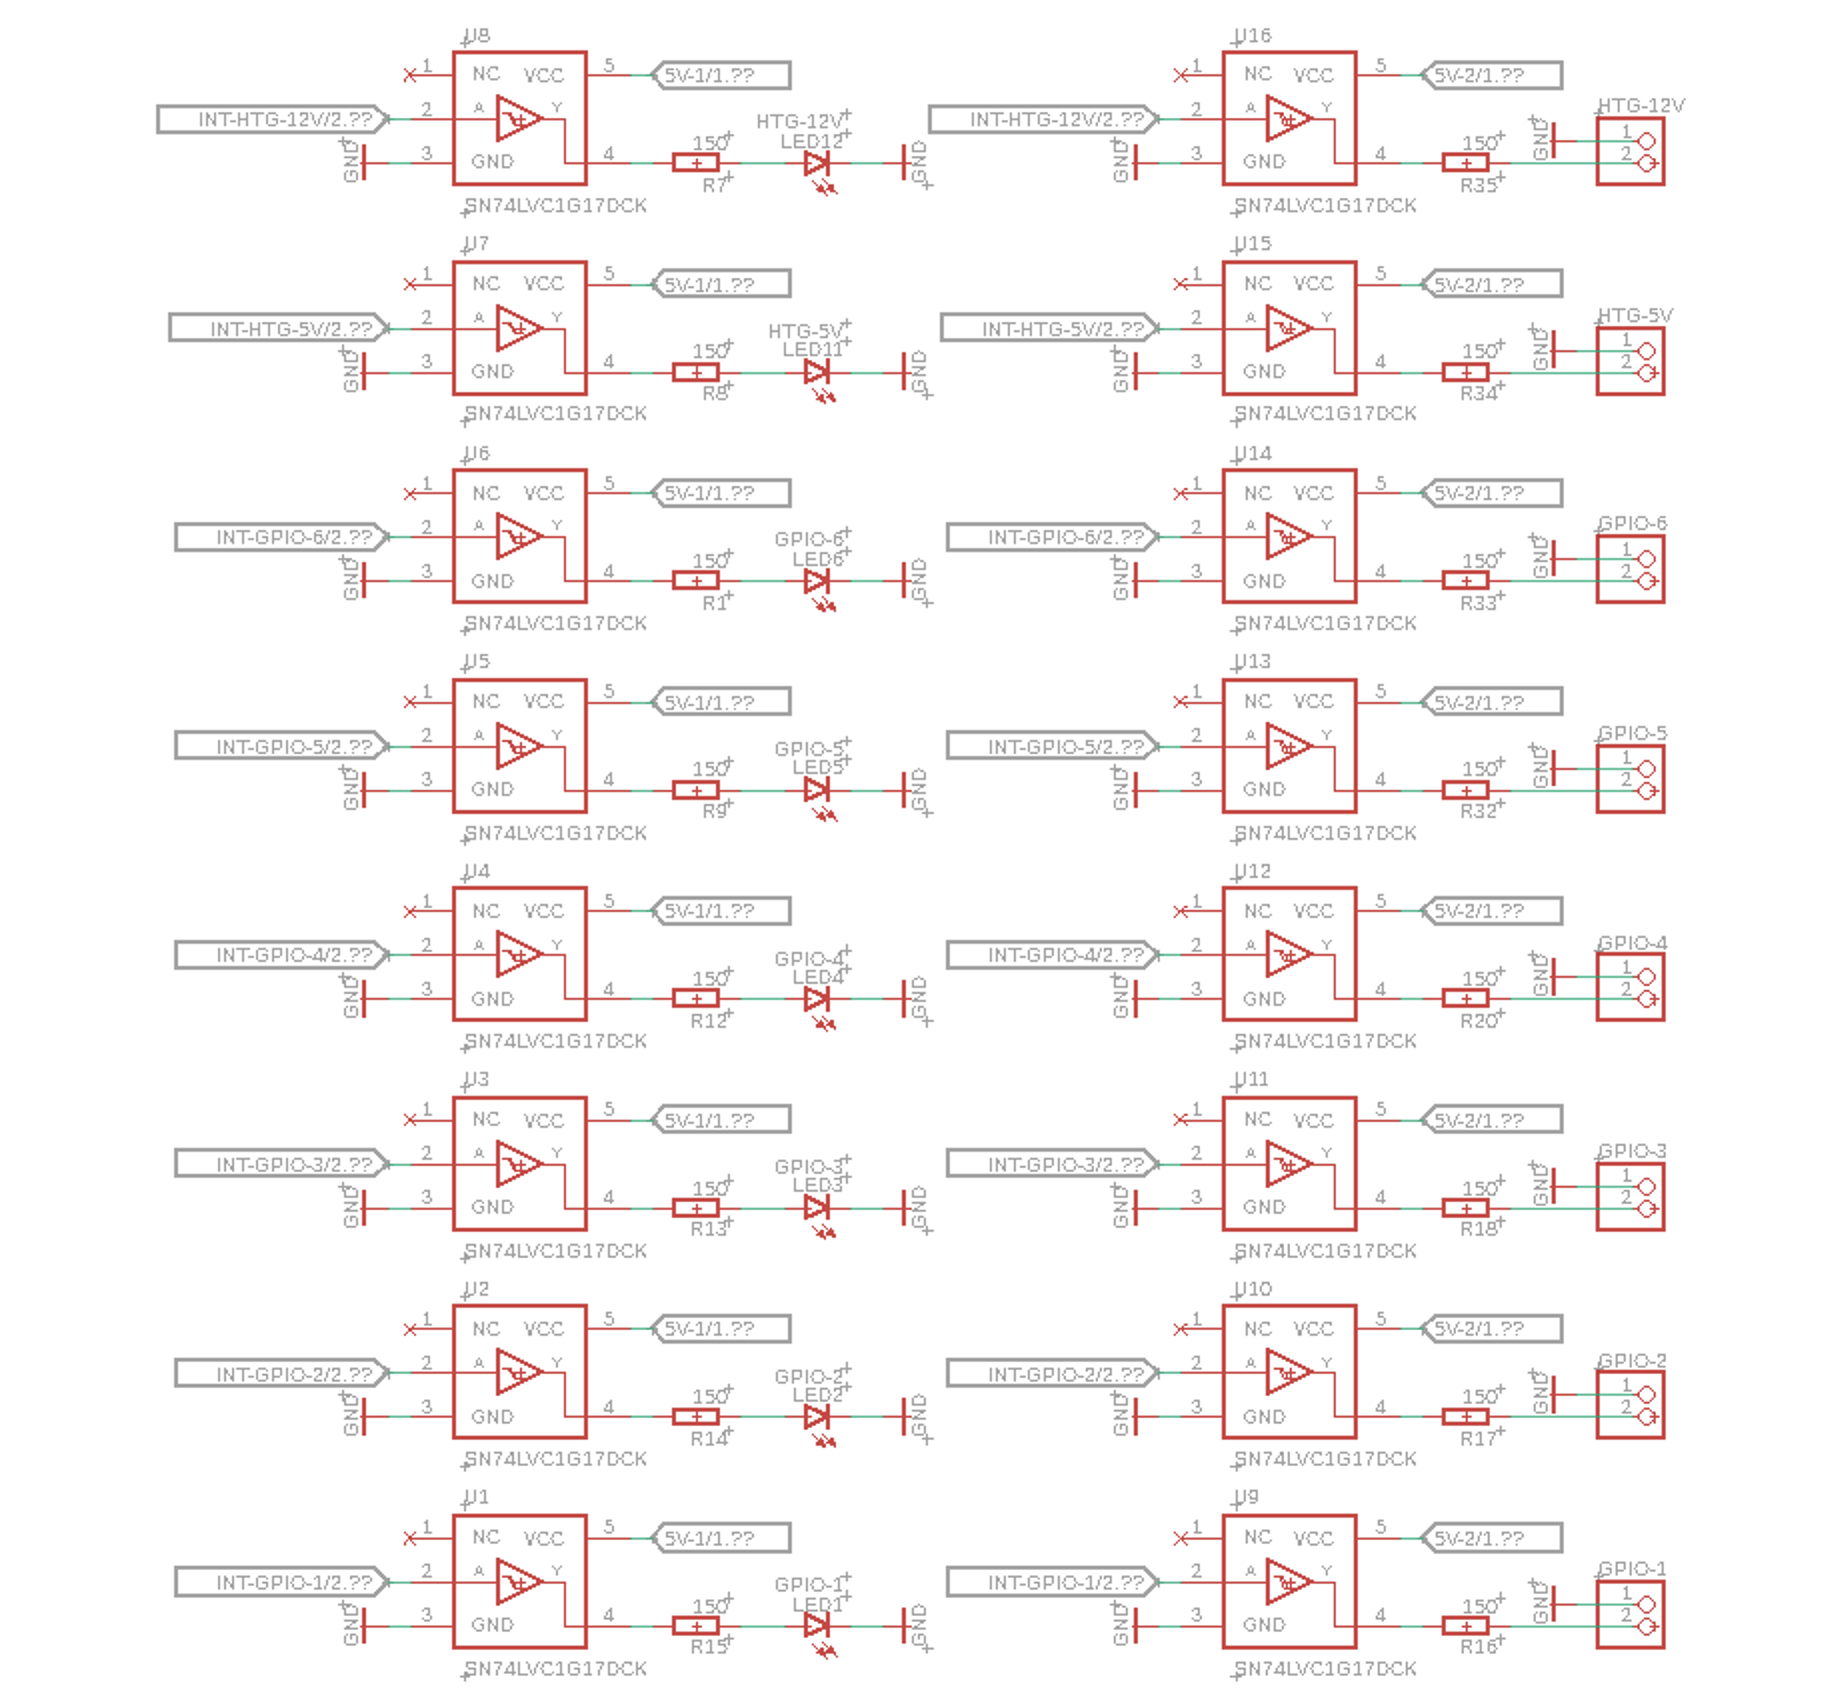
\includegraphics[width=1.1\linewidth]{figures/Interface_board_schematic_3.png}
\caption{Interface Board Schematic Part 3}
\label{fig:interface_sch3}
\end{figure}
%

\end{document}
